\documentclass[10pt, a4paper, twoside]{article}
\usepackage{fontspec}
\usepackage{realscripts}
\setmainfont[
  BoldFont=CambriaB,
  BoldItalicFont=CambriaZ,
  Numbers={OldStyle, Proportional}, 
  Ligatures={TeX, Common}, 
  SmallCapsFeatures={Letters=SmallCaps},
  %Contextuals=WordFinal,
            ]{Cambria}
\setmonofont[Scale=MatchLowercase]{Consolas}
\newcommand{\textcsc}[1]{{\addfontfeature{Letters=UppercaseSmallCaps}#1}}

\usepackage[dvipsnames]{xcolor}
\usepackage{accsupp}
\newfontfamily\cuneiformComposite{CuneiformComposite.ttf}
\newfontfamily\originalNoto{NotoSansCuneiform-UN-Swapped.ttf}
\newfontfamily\xsuxfont{NotoSansCuneiform-egg.ttf}
\newfontfamily\obfont{Santakku.ttf}
\newfontfamily\nafont{Assurbanipal.ttf}
\newfontfamily\nbfont{Esagil.ttf}
\newfontfamily\hantfont{NotoSerifTC-Regular.ttf}
%\usepackage{arabluatex}

\newfontfamily\arabicfont[Script=Arabic]{ScheherazadeNew-Regular.ttf}
%\newcommand{\textarabic}[1]{%\BeginAccSupp{method=pdfstringdef,unicode,ActualText={#1}}%
%\bgroup\textdir TRT%
%\arabfont #1%
%\egroup%\EndAccSupp{}
%}

\newfontfamily\proposalfont{Archaic-Cuneiform-Numerals.ttf}

\newcommand\oneAšC{{\proposalfont\symbol{"12550}}} % 𒀸
\newcommand\twoAšC{{\proposalfont\symbol{"12551}}} % 𒐀
\newcommand\threeAšC{{\proposalfont\symbol{"12552}}} % 𒐁
\newcommand\fourAšC{{\proposalfont\symbol{"12553}}} % 𒐂
\newcommand\fiveAšC{{\proposalfont\symbol{"12554}}} % 𒐃
\newcommand\sixAšC{{\proposalfont\symbol{"12555}}} % 𒐄
\newcommand\sevenAšC{{\proposalfont\symbol{"12556}}} % 𒐅
\newcommand\eightAšC{{\proposalfont\symbol{"12557}}} % 𒐆
\newcommand\nineAšC{{\proposalfont\symbol{"12558}}} % 𒐇
\newcommand\oneDišC{{\proposalfont\symbol{"12559}}}
\newcommand\twoDišC{{\proposalfont\symbol{"1255A}}}
\newcommand\threeDišC{{\proposalfont\symbol{"1255B}}}
\newcommand\fourDišC{{\proposalfont\symbol{"1255C}}}
\newcommand\fiveDišC{{\proposalfont\symbol{"1255D}}}
\newcommand\sixDišC{{\proposalfont\symbol{"1255E}}}
\newcommand\sevenDišC{{\proposalfont\symbol{"1255F}}}
\newcommand\eightDišC{{\proposalfont\symbol{"12560}}}
\newcommand\nineDišC{{\proposalfont\symbol{"12561}}}
\newcommand\oneUC{{\proposalfont\symbol{"12562}}}
\newcommand\twoUC{{\proposalfont\symbol{"12563}}}
\newcommand\threeUC{{\proposalfont\symbol{"12564}}}
\newcommand\fourUC{{\proposalfont\symbol{"12565}}}
\newcommand\fiveUC{{\proposalfont\symbol{"12566}}}
\newcommand\sixUC{{\proposalfont\symbol{"12567}}}
\newcommand\sevenUC{{\proposalfont\symbol{"12568}}}
\newcommand\eightUC{{\proposalfont\symbol{"12569}}}
\newcommand\nineUC{{\proposalfont\symbol{"1256A}}}
\newcommand\oneŊešTwoC{{\proposalfont\symbol{"1256B}}}
\newcommand\twoŊešTwoC{{\proposalfont\symbol{"1256C}}}
\newcommand\threeŊešTwoC{{\proposalfont\symbol{"1256D}}}
\newcommand\fourŊešTwoC{{\proposalfont\symbol{"1256E}}}
\newcommand\fiveŊešTwoC{{\proposalfont\symbol{"1256F}}}
\newcommand\sixŊešTwoC{{\proposalfont\symbol{"12570}}}
\newcommand\sevenŊešTwoC{{\proposalfont\symbol{"12571}}}
\newcommand\eightŊešTwoC{{\proposalfont\symbol{"12572}}}
\newcommand\nineŊešTwoC{{\proposalfont\symbol{"12573}}}
\newcommand\oneŊešʾuC{{\proposalfont\symbol{"12574}}}
\newcommand\twoŊešʾuC{{\proposalfont\symbol{"12575}}}
\newcommand\threeŊešʾuC{{\proposalfont\symbol{"12576}}}
\newcommand\fourŊešʾuC{{\proposalfont\symbol{"12577}}}
\newcommand\fiveŊešʾuC{{\proposalfont\symbol{"12578}}}
\newcommand\oneŠarTwoC{{\proposalfont\symbol{"12579}}}
\newcommand\twoŠarTwoC{{\proposalfont\symbol{"1257A}}}
\newcommand\threeŠarTwoC{{\proposalfont\symbol{"1257B}}}
\newcommand\fourŠarTwoC{{\proposalfont\symbol{"1257C}}}
\newcommand\fiveŠarTwoC{{\proposalfont\symbol{"1257D}}}
\newcommand\sixŠarTwoC{{\proposalfont\symbol{"1257E}}}
\newcommand\seveŠarTwoC{{\proposalfont\symbol{"1257F}}}
\newcommand\eightŠarTwoC{{\proposalfont\symbol{"12580}}}
\newcommand\nineŠarTwoC{{\proposalfont\symbol{"12581}}}
\newcommand\oneŠarʾuC{{\proposalfont\symbol{"12582}}}
\newcommand\twoŠarʾuC{{\proposalfont\symbol{"12583}}}
\newcommand\threeŠarʾuC{{\proposalfont\symbol{"12584}}}
\newcommand\fourŠarʾuC{{\proposalfont\symbol{"12585}}}
\newcommand\fiveŠarʾuC{{\proposalfont\symbol{"12586}}}
\newcommand\oneEighthIkuC{{\proposalfont\symbol{"12587}}}
\newcommand\oneEighthIkuCV{{\proposalfont\symbol{"12588}}}
\newcommand\oneQuarterIkuC{{\proposalfont\symbol{"12589}}}
\newcommand\oneQuarterIkuCV{{\proposalfont\symbol{"1258A}}}
\newcommand\oneHalfIkuCV{{\proposalfont\symbol{"1258B}}}
\newcommand\oneEšeThreeC{{\proposalfont\symbol{"1258C}}}
\newcommand\oneBurʾuC{{\proposalfont\symbol{"1258E}}}
\newcommand\oneBanTwoC{{\proposalfont\symbol{"12593}}}
\newcommand\twoBanTwoC{{\proposalfont\symbol{"12594}}}
\newcommand\threeBanTwoC{{\proposalfont\symbol{"12595}}}
\newcommand\oneNFiftyOneC{{\proposalfont\symbol{"1259A}}}
\newcommand\oneNFiftyFourC{{\proposalfont\symbol{"125A3}}}
\newcommand\oneNFiftySixC{{\proposalfont\symbol{"125A8}}}
\newcommand\fourBanTwoC{{\proposalfont\symbol{"12596}}}
\newcommand\fiveBanTwoC{{\proposalfont\symbol{"12597}}}
\newcommand\oneThirdCV{{\proposalfont\symbol{"12598}}}
\newcommand\twoThirdsCV{{\proposalfont\symbol{"12599}}}
\newcommand\oneNTwentyFour{{\proposalfont\symbol{"125AA}}}
\newcommand\oneNTwentySix{{\proposalfont\symbol{"125AB}}}
\newcommand\oneNTwentyEight{{\proposalfont\symbol{"125AC}}}
\newcommand\oneNTwentyNineA{{\proposalfont\symbol{"125AD}}}
\newcommand\oneNTwentyNineB{{\proposalfont\symbol{"125AE}}}
\newcommand\oneNTwentyThirtyA{{\proposalfont\symbol{"125AF}}}
\newcommand\oneNTwentyThirtyC{{\proposalfont\symbol{"125B0}}}
\newcommand\oneNTwentyThirtyD{{\proposalfont\symbol{"125B1}}}
\newcommand\oneNTwentyThirtyE{{\proposalfont\symbol{"125B2}}}
\newcommand\oneNTwentyThirtyOne{{\proposalfont\symbol{"125B3}}}
\newcommand\oneNTwentyThirtyTwo{{\proposalfont\symbol{"125B4}}}
\newcommand\oneNTwentyThirtyThree{{\proposalfont\symbol{"125B5}}}
\newcommand\oneNThirtyA{{\proposalfont\symbol{"125AF}}}
\newcommand\oneNThirtyC{{\proposalfont\symbol{"125B0}}}
\newcommand\oneNThirtyNineA{{\proposalfont\symbol{"125B6}}}
\newcommand\oneNThirtyNineB{{\proposalfont\symbol{"125BA}}}
\newcommand\oneNFour{{\proposalfont\symbol{"12605}}}
\newcommand\threeNThirtyFive{{\proposalfont\symbol{"125CE}}}
\newcommand\fourNThirtyFive{{\proposalfont\symbol{"125CF}}}
\newcommand\fiveNThirtyFive{{\proposalfont\symbol{"125D0}}}
\newcommand\oneNFortyOne{{\proposalfont\symbol{"12601}}}
\newcommand\oneNSevenB{{\proposalfont\symbol{"12648}}}
\newcommand\oneNNine{{\proposalfont\symbol{"12642}}}
\newcommand\oneNEleven{{\proposalfont\symbol{"12643}}}
\newcommand\oneNTwelve{{\proposalfont\symbol{"12644}}}
\newcommand\oneNTwo{{\proposalfont\symbol{"125BE}}}
\newcommand\sixNTwo{{\proposalfont\symbol{"125C3}}}
\newcommand\oneNFifteen{{\proposalfont\symbol{"125C7}}}
\newcommand\oneNThirtyFive{\proposalfont\symbol{"125CC}}

\newcommand{\nhphantom}[1]{\sbox0{#1}\hspace{-\the\wd0}}

\usepackage{afterpage}
\usepackage{float}

\usepackage{tikz-cd}
\usetikzlibrary{babel}

\usepackage{polyglossia}
\setdefaultlanguage[variant=british]{english}
\setotherlanguages{greek,german,russian,french,arabic}
\usepackage{luabidi}
% We use the english/american quote style, i.e., outer double quotes and inner
% single quotes, but british typographic rules (punctuation after the quotation
% marks).
\usepackage[style=english/american]{csquotes}

\usepackage{mathtools}
\usepackage{empheq}

\ExplSyntaxOn

\NewDocumentCommand \FribergFullStopTwentySevenTag { m }
  {
    \regex_match:nnTF { 27 } { #1 }
      { (#1). }
      { (#1) }
  }

\ExplSyntaxOff
\newtagform{fribergFullStopTwentySeven}[\FribergFullStopTwentySevenTag]{}{}


\usepackage{unicode-math}
\setmathfont[Scale=MatchLowercase, math-style=ISO]{Cambria Math}
\setmathfontface\unifrak{UnifrakturMaguntia.ttf}[Scale=MatchLowercase]

\usepackage[colorlinks,allcolors=Periwinkle]{hyperref}
\usepackage[backend=biber,giveninits=true,maxnames=100,style=alphabetic,maxalphanames=4,doi=true,url=false,eprint=true,labelalpha=true,dateusetime=true]{biblatex}
\addbibresource{artefacts.bib}
\addbibresource{bibliography.bib}
\addbibresource{unicode.bib}
\DeclareSourcemap{
  \maps{
    \map{
      \step[fieldsource=keywords, match=\regexp{reference}, final]
      \step[fieldsource=entrykey, final]
      \step[fieldset=shorthand, origfieldval]
    }
    \map{
      \step[fieldsource=keywords, match=\regexp{unicode}, final]
      \step[fieldsource=eprint, final]
      \step[fieldset=shorthand, origfieldval]
    }
    \map{
      \pertype{artwork}
      \step[fieldsource=eprint, final]
      \step[fieldset=shorthand, origfieldval]
    }
  }
}

% Allow breaking in numbers and after lower and upper case letters in bibliography
% URLs, see https://tex.stackexchange.com/a/134281.
% We use fairly low values to avoid unsightly spacing:
% http : / / example . com is not an improvement over http://ex-
% ample.com.  We prefer breaking in numbers and uppercase letters, which are often
% IDs, rather than lowercase letters, which sometimes form meaningful words, or at
% least tokens that are not customarily broken, e.g. the protocol.
\setcounter{biburlnumpenalty}{100}
\setcounter{biburllcpenalty}{500}
\setcounter{biburlucpenalty}{100}
\renewcommand\UrlFont{}

\AtEveryBibitem{\clearlist{language}}  % TODO(egg): Why are we doing this?

\DeclareBibliographyAlias{artwork}{report}

\newcommand\UTCdoc[1]{\href{https://www.unicode.org/cgi-bin/GetMatchingDocs.pl?#1}{#1}}
\newcommand\WGtwodoc[1]{\href{http://www.unicode.org/cgi-bin/GetMatchingWG2Docs.pl?#1}{#1}}

\DeclareFieldFormat{doi}{%
  \newline
  \mkbibacro{DOI}\addcolon\space
    \ifhyperref
      {\href{https://doi.org/#1}{#1}}
      {#1}}
\DeclareFieldFormat{eprint:cnki}{%
  \newline
  \mkbibacro{CNKI}\addcolon\space
    \ifhyperref
      {\href{http://www.cnki.com.cn/Article/CJFDTOTAL-#1.htm}{#1}}
      {#1}}
\DeclareFieldFormat{eprint:utc}{%
  \newline
  \mkbibacro{UTC}\addcolon\space
    \ifhyperref
      {\UTCdoc{#1}}
      {#1}}
\DeclareFieldFormat{eprint:wg2}{%
  \newline
  \mkbibacro{ISO/IEC JTC~1/SC~2/WG~2}\addcolon\space
    \ifhyperref
      {\WGtwodoc{#1}}
      {#1}}
\DeclareFieldFormat{eprint:cdli}{%
  \newline
  \mkbibacro{CDLI}\addcolon\space
    \ifhyperref
      {\href{https://cdli.ucla.edu/#1}{#1}}
      {#1}}
\DeclareFieldFormat{eprint:ebda}{%
  \newline
  Eb\textsc{da}\addcolon\space
    \ifhyperref
      {\href{http://ebda.cnr.it/tablet/view/#1}{#1}}
      {#1}}
\DeclareFieldFormat{eprint:oracc}{%
  \newline
  \mkbibacro{ORACC}\addcolon\space
    \ifhyperref
      {\href{http://oracc.org/#1}{#1}}
      {#1}}
\DeclareFieldFormat{eprint:etcsl}{%
  \newline
  \mkbibacro{ETCSL}
    \ifhyperref
      {transliteration: \href{https://etcsl.orinst.ox.ac.uk/cgi-bin/etcsl.cgi?text=c.#1\&display=Crit\&charenc=gtilde}{c.#1};
       translation: \href{https://etcsl.orinst.ox.ac.uk/cgi-bin/etcsl.cgi?text=t.#1\&display=Crit\&charenc=gtilde}{t.#1}}
      {transliteration: {c.#1}
       translation: {t.#1}}}
\DeclareFieldFormat{eprint:louvre}{%
  \newline
  Louvre Collections\addcolon\space
    \ifhyperref
      {\href{https://collections.louvre.fr/#1}{#1}}
      {#1}}
\DeclareFieldFormat{eprint}{%
  \newline
    \ifhyperref
      {\href{#1}{\nolinkurl{#1}}}
      {\nolinkurl{#1}}}
\DeclareFieldFormat{isbn}{%
  \newline
  \mkbibacro{ISBN}\addcolon\space#1}
\renewcommand{\relateddelim}{\newunitpunct}
      
\newcommand{\idest}{\emph{i.e.}}
\newcommand{\exempligratia}{\emph{e.g.}}
\newcommand{\obverse}{obv.}
\newcommand{\reverse}{\IfFontFeatureActiveTF{Numbers=Tabular}{\rlap{rev.}\hphantom{obv.}}{rev.}}
\newcommand{\recto}{\emph{\IfFontFeatureActiveTF{Numbers=Tabular}{\rlap{recto}\hphantom{verso}}{recto}}}
\newcommand{\verso}{\emph{verso}}
\newcommand{\withnote}{n.}
\newcommand{\withnotes}{nn.}

\usepackage{multirow}

\usepackage{epigraph}
\renewcommand{\epigraphsize}{\footnotesize}
\renewcommand{\textflush}{flushepinormal}
%\setlength\epigraphrule{0pt}
\epigraphnoindent

\usepackage{enumitem}
\renewcommand\labelitemi{---}
\renewcommand\labelitemii{---}

\usepackage[style=iso]{datetime2}

\hyphenation{cunei-form}
\usepackage{microtype}
\tikzcdset{
arrow style=math font,
}

\renewcommand{\topfraction}{0.9}

\usepackage{luacolor}
\usepackage{lua-ul}
\LuaULSetHighLightColor{yellow}
\newcommand{\removed}[1]{\highLight{\strikeThrough{#1}}}
\newcommand{\changed}[1]{\highLight{#1}}

\usepackage{pdfpages}

\title{Archaic cuneiform numerals}
\author{Robin Leroy, Anshuman Pandey, and Steve Tinney}

\begin{document}

\maketitle

\tableofcontents

\section{Summary}

This document proposes encoding, at U+12550--U+12585, 310 numerals
used in the fourth millennium (Uruk IV and Uruk III periods) and Early Dynastic period in conjunction
with the Sumero-Akkadian cuneiform script\footnote{\cite{ISO15924}: Xsux, Script property value long name: Cuneiform; encoded since Unicode Version 5.0.}
and the proto-cuneiform script\footnote{\cite{ISO15924}: Pcun, not yet encoded.}.
The proposed characters are listed in §\ref{proposal}.
Most of them were listed in \cite{L2/23-190}.
The present document provides a more detailed rationale for their encoding
and additional information about their identity and usage,
both as part of the rationale and in §\ref{extraIdentity}. Some characters have been
removed, in some cases because they are non-encodable variants,
in others because their encodability should be considered as part of the proto-cuneiform proposal;
these are discussed in §\ref{notIncluded}.
The glyphs have also been reworked, and
additional characters used in the Early Dynastic period have been added.

The non-numeric signs of proto-cuneiform will be the subject of a separate proposal;
we need only note here that the divergence between the approaches to character identity
in modern scholarship requires that proto-cuneiform be disunified from cuneiform:
proto-cuneiform is effectively treated as an undeciphered script.
In contrast, the cuneiform encoding model requires an understanding of the text to correctly encode it.

However, the \emph{numerals} used in proto-cuneiform should be unified with
ones used in the Early Dynastic period, for the reasons set forth in
§\ref{unificationRationale}.
The proposed ``curved'', or ``curviform'', numerals\footnote{%
Impressed into clay using cylindrical styli,
held either perpendicular to the tablet, yielding
\oneUC{} (small stylus) or
\oneŠarTwoC{} (large stylus),
or at a shallower angle:
\oneAšC, \oneDišC{} (small stylus),
\oneŊešTwoC{}, \oneNThirtyNineA{} (large stylus).
Some numerals are composed of multiple such impressions,
\exempligratia, \oneŊešʾuC.
The terms ``curved'', ``curviform'', ``curvilinear'', and ``round''
can be found in the literature.
We avoid the term ``round'' here as it has other meanings
in the context of numbers.
We use ``curviform'' in this document as, being the least
common term, it is least likely to lead to confusion,
and ``CURVED'' in the character names for consistency
with documentation about the modifier @c used in machine
readable ATF transliterations \cite{inlineATF}.}
should however \emph{not} be unified with
the already-encoded cuneiform numerals\footnote{%
Impressed into clay using a stylus with a trihedral end:
{\xsuxfont 𒀸} (stylus held horizontally),
{\xsuxfont 𒁹} (vertically),
{\xsuxfont 𒀹} (diagonally)
{\xsuxfont 𒌋} (with the head of the stylus),
{\xsuxfont 𒐕} (stylus pressed deeper, forming a larger wedge),
{\xsuxfont 𒐞} (combining {\xsuxfont 𒐕} and {\xsuxfont 𒌋}), etc.}.
Since the encoding proposals for the cuneiform script
twenty years ago provisionally considered the curviform numerals
to be glyph variants of the cuneiform numerals,
a detailed rationale is provided in §\ref{disunificationRationale},
including compatibility considerations in §\ref{compatibility}.

The overall picture of unifications and disunifications over time is illustrated in table~\ref{tableUnificationsDisunifications}.
The Script\_Extensions property assignments in §\ref{properties} reflect the overlap.
Many of these numerals are also used in proto-Elamite\footnote{\cite{ISO15924}: Pelm, not yet encoded.} texts,
where they are treated as identical characters in scholarship on proto-Elamite,
so that they should be unified with the ones proposed in \cite{L2/23-196}.
However, in the interest of time, we do not provide a detailed rationale for this unification in this document,
and we are not proposing that the numerals be given the corresponding Script\_Extensions property value for now.
Neither do we propose encoding any numerals that are solely attested in proto-Elamite texts,
or well-attested in proto-Elamite texts but insufficiently attested in Uruk---those are discussed in §\ref{notIncluded}.

\begin{table}[htbp]
\begin{center}
\begin{tabular}{ l | l | l | l |} \cline{2-4}
                                                & Uruk III \& earlier & ED – Ur III                         & OB \& later    \\\hline
\multicolumn{1}{|c|}{\multirow{2}{*}{Numerals}} & \multicolumn{2}{|c|}{This proposal}                       &                \\\cline{2-4}
\multicolumn{1}{|c|}{}                          &                     & \multicolumn{2}{|c|}{\multirow{2}{*}{Existing Xsux}} \\\cline{1-2}
\multicolumn{1}{|c|}{Non-numeric signs}         & Future Pcun         & \multicolumn{2}{|c|}{}                               \\\hline
\end{tabular}
\caption{Usage of existing, proposed, and future characters across functions and time periods.}
\end{center}
\label{tableUnificationsDisunifications}
\end{table}

\section{Proposed changes to the Standard}
\label{proposal}
\subsection{Core specification text}

Amend \cite[§11.1.2, \emph{sub} ``\href{https://www.unicode.org/versions/Unicode16.0.0/core-spec/chapter-11/\#G26965}{Cuneiform Numerals}'']{Unicode16}, as follows:
\begin{quotation}
  \noindent\textbf{\textit{Cuneiform Numerals.}} In general, numerals \changed{
  that also have a phonetic, logographic, or determinative value are encoded in the
  main Cuneiform block; as a result, some series of numerals, such as
  \smash{\cuneiformComposite 𒁹}--\smash{\cuneiformComposite 𒐎} $1$(diš)--$9$(diš) or
  \smash{\cuneiformComposite 𒌋}--\smash{\cuneiformComposite 𒐔} $1$(u)--$9$(u),
  are split across the two blocks.
  Numerals} have been encoded separately
  from signs that are visually identical but\removed{ semantically different}\changed{ etymologically unrelated}
  (for example, U+\textcsc{1244F} {\cuneiformComposite 𒑏} \textcsc{CUNEIFORM NUMERIC SIGN ONE BAN2},
  U+\textcsc{12450} {\cuneiformComposite 𒑐} \textcsc{CUNEIFORM NUMERIC SIGN TWO BAN2},
  and so on,
  versus U+\textcsc{12226} {\cuneiformComposite 𒑏} \textcsc{CUNEIFORM SIGN MASH},
  U+\textcsc{1227A} {\cuneiformComposite 𒑐} \textcsc{CUNEIFORM SIGN PA}, and so on).

  \changed{The relation between series of numerals depends on the metrological system;
  for instance, when counting talents, written \smash{\cuneiformComposite 𒄘} (a unit of weight, approximately $30$~kg),
  \smash{\cuneiformComposite 𒀸𒄘} is used for ``one talent'', and \smash{\cuneiformComposite 𒌋𒄘} for ``ten talents''.
  However, when measuring areas, the area \smash{\cuneiformComposite 𒌋𒃷} (one \emph{būrum}) is eighteen times
  \smash{\cuneiformComposite 𒀸𒃷} (one \emph{ikûm}, approximately $3600~\mathrm{m}^2$).
  The Numeric\_Value property assignment of a cuneiform numeral therefore reflects only
  its relation to the first numeral in its series,
  rather than the absolute numeric value that it might represent.
  For instance, the number ``fifty'' is written \smash{\cuneiformComposite 𒐐},
  but U+\textcsc{12410} \smash{\cuneiformComposite 𒐐} \textcsc{CUNEIFORM NUMERIC SIGN FIVE U}
  has Numeric\_Value=$5$, as it is $5\times\text{\cuneiformComposite 𒌋}$.}

  \changed{In the third millennium, and especially in the Early Dynastic period,
  some numerals are written using a cylindrical tool, rather than the cuneiform stylus,
  forming curved rather than cuneiform numerals (\oneAšC{} rather than {\cuneiformComposite 𒀸}).
  The cuneiform numerals are descended from these curved numerals.
  However, in the Early Dynastic period, the curved numerals contrast with the cuneiform ones,
  and are used together with them in several metrological systems; they are therefore separately encoded.
  Most curved numerals are encoded in the Archaic Cuneiform Numerals block, with the exception of two fractions
  in the Cuneiform Numbers and Punctuation block:
  U+\textcsc{1245D} \smash{\cuneiformComposite 𒑝} \textcsc{CUNEIFORM NUMERIC SIGN ONE THIRD VARIANT FORM A}
  and U+\textcsc{1245E} \smash{\cuneiformComposite 𒑞} \textcsc{CUNEIFORM NUMERIC SIGN TWO THIRDS VARIANT FORM A},
  the curved counterparts of U+\textcsc{1245A} \smash{\cuneiformComposite 𒑚} \textcsc{CUNEIFORM NUMERIC SIGN ONE THIRD DISH}
  and U+\textcsc{1245B} \smash{\cuneiformComposite 𒑛} \textcsc{CUNEIFORM NUMERIC SIGN TWO THIRDS DISH}.}
\end{quotation}
Add after \cite[§\href{https://www.unicode.org/versions/Unicode16.0.0/core-spec/chapter-11/\#G27840}{11.1.3}]{Unicode16}:
\begin{quotation}
\noindent{\large\textbf{\textit{11.1.4 Archaic Cuneiform Numerals: U+12550–U+1268F}}}
This block contains numerals used in the fourth millennium and third millennium.
The numerals that are used in the fourth millennium and Early Dynastic I--II period
(2900--2700 \textcsc{BCE}) are named according to the conventions
of the Berlin \emph{Archaische Texte aus Uruk} (ATU) project, with names such as
U+12550 \oneAšC{} \textcsc{CUNEIFORM NUMERIC SIGN ONE N01} or
U+\textcsc{125B6} \oneNThirtyNineA{} \textcsc{CUNEIFORM NUMERIC SIGN ONE N39A}.
For the signs that are also used in the third millennium,
informative aliases provide correspondences to more common third millennium conventions,
such as ``1 aš curved'' for U+12550 \oneAšC{} \textcsc{CUNEIFORM NUMERIC SIGN ONE N01}.
The numerals that are only used starting in the Early Dynastic III period,
where the ATU notation is not used, are named in the same fashion as
the numerals of the Cuneiform Numbers and Punctation block.

The curved numerals are produced using cylindrical tools of two different sizes,
producing small curved indents (\oneAšC{}, \oneDišC{}, and \oneUC),
and large ones (\oneŊešTwoC{}, \oneNThirtyNineA{}, and \oneŠarTwoC).
These can be combined, as in U+12574 \oneŊešʾuC{} \textcsc{CUNEIFORM NUMERIC SIGN ONE N48},
U+12582 \oneŠarʾuC{} \textcsc{CUNEIFORM NUMERIC SIGN ONE N50},
or U+\textcsc{125A3} \oneNFiftyFourC{} \textcsc{CUNEIFORM NUMERIC SIGN ONE N54}.
Consistent sizing is important to identifying these characters, as there is
no visual distinction other than size between, for instance,
U+\textcsc{12566} \fiveUC{} \textcsc{CUNEIFORM NUMERIC SIGN FIVE N14} and
 U+\textcsc{1257D} \fiveŠarTwoC{} \textcsc{CUNEIFORM NUMERIC SIGN FIVE N45}.
The reference glyphs of some of the larger signs have been resized to fit
in the code charts cells, but fonts for these characters should retain consistent size
across the numeral series.

\begin{quote}
\textit{Editor's note: I have not yet done that resizing.
The dashed-box convention for wide dashes, see \cite[§24.1.2, \emph{sub}
``\href{https://www.unicode.org/versions/Unicode16.0.0/core-spec/chapter-24/\#G8188}{Dashed Box Convention}'']{Unicode16}
should probably not be extended to these,
since numbers enclosed in a real dashed box are a thing in proto-Elamite texts.}
\end{quote}

The Numeric\_Value assignments follow the same principles as in the Cuneiform Numbers and Punctuation block.
Numerals used in the third millennium have the Cuneiform script property value;
numerals used only in the fourth millennium have the Proto-Cuneiform script property value.
Numerals used in both the fourth and third millennium have both scripts in their Script\_Extensions values.

\noindent\textbf{\textit{The sign ŠAR₂.}} When used logographically, the sign
ŠAR₂ has the same (cuneiform) appearance as U+\textcsc{1212D} {\cuneiformComposite 𒄭}
\textcsc{CUNEIFORM SIGN HI} in all but the most archaizing Early Dynastic texts.
The character U+\textcsc{122B9} \textsc{cuneiform sign shar2} should be used for logographic šar₂,
whether cuneiform or curved. Most period-specific fonts will have the same cuneiform
glyph for U+\textcsc{122B9} and U+\textcsc{1212D}.
In the Early Dynastic period, numeric 1 šar₂ is typically written with a curved glyph,
contrasting with logographic šar₂. U+\textcsc{12579} \oneŠarTwoC{} \textcsc{CUNEIFORM
NUMERIC SIGN ONE N45} should be used for curved 1 šar₂.
In later periods, long after ŠAR₂ and ḪI have merged, even numeric 1 šar₂ has a cuneiform glyph.
U+\textcsc{122B9} \textsc{cuneiform sign shar2} should be used for cuneiform 1 šar₂.

The reference glyph for U+\textcsc{122B9} {\cuneiformComposite 𒊹} \textsc{cuneiform sign shar2}
is curved, reflecting the rarer and more archaic practice, instead of cuneiform as it would
be in the Ur III period, so as to distinguish it from
U+\textcsc{1212D} {\cuneiformComposite 𒄭} \textcsc{CUNEIFORM SIGN HI}.
\end{quotation}
% Amend \cite[§24.1.2, \emph{sub} ``\href{https://www.unicode.org/versions/Unicode16.0.0/core-spec/chapter-24/\#G8188}{Dashed Box Convention}'']{Unicode16},
% third paragraph, as follows:
% \begin{quotation}
%   In a few cases of very wide \removed{punctuation }characters that do not naturally fit into a code chart cell,
%   the representative glyph may be shown with an artificially narrow shape,
%   displayed inside the dashed box, with or without additional annotation,
%   to indicate this adjustment of shape.
% \end{quotation}
\subsection{Code charts}
The code charts for the proposed block,
including the character names list with proposed informative aliases, cross references, and informative notes,
are shown on the following pages.
\vspace{0pt plus 0.5fill}
\begin{center}This space for rent.\end{center}
\vfill
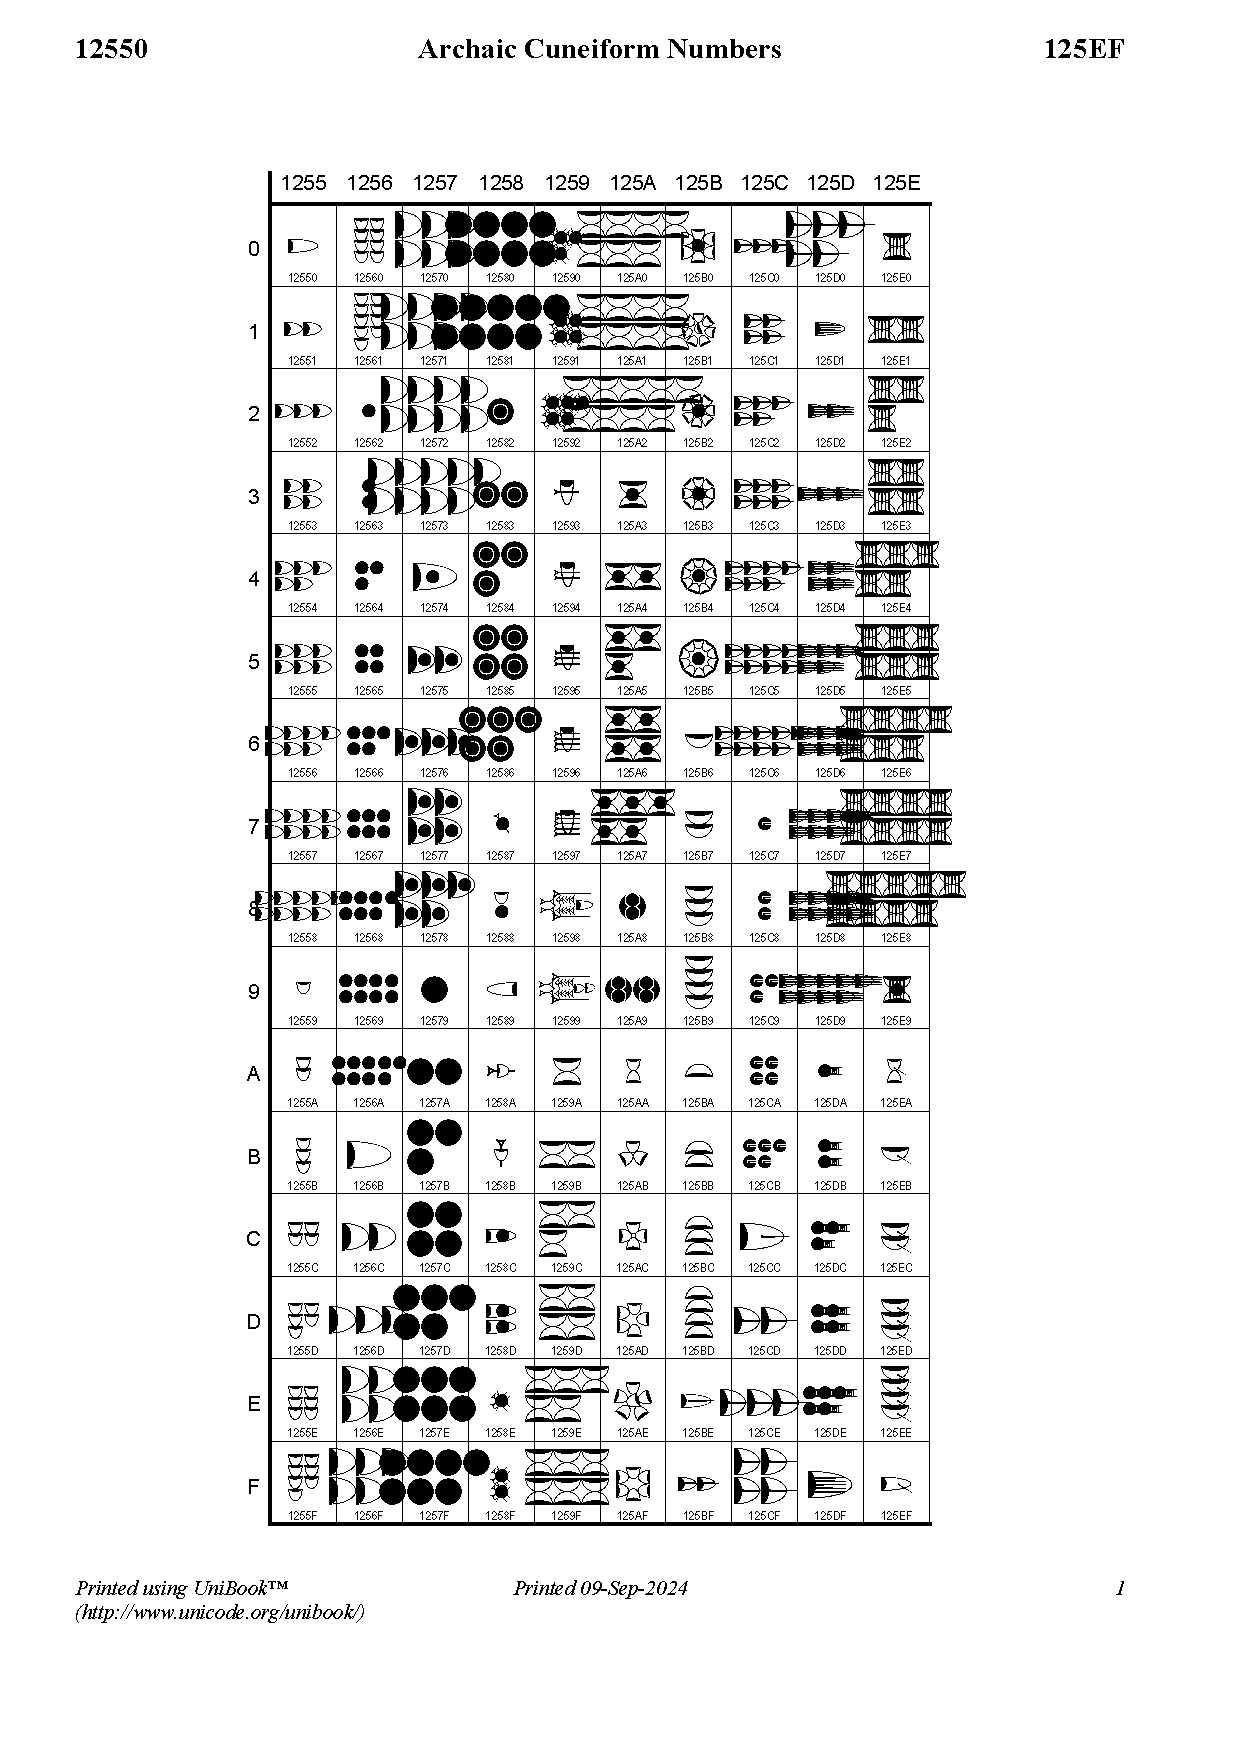
\includepdf[pages=-]{chart.pdf}
\subsection{Properties}
\label{properties}
\section{Rationale for curviform--cuneiform disunification}
\label{disunificationRationale}
The numbering systems that use cuneiform numerals are descended from the ones that use curviform numerals,
and many of the cuneiform signs have clear curviform counterparts across this transition.
Co-occurrences are sometimes described by analogy to distinctions that are not the realm of plain text,
as in \cite[215]{Powell1972} ``in the same fashion as we use black and red ink'';
however, we must bear in mind that such analogies are not made in the context of character encoding discussions.
In 2004, the curviform numerals were deemed unencodable for the time being; however,
closer inspection reveals that the distinction functions less like markup than was argued at the time,
and that the unification is problematic.

\subsection{The cuneiform encoding model}
\label{xsuxModel}
As outlined in, \exempligratia, \cite{UTR56}, the cuneiform encoding model is diachronic;
each character may have wildly different glyphs depending on time period and region.
For instance, the sign IM
may resemble {\cuneiformComposite 𒅎} in texts from Early Dynastic IIIa Šuruppag as in the character code
charts,
{\cuneiformComposite 𒉎} % TODO(egg): Do something clever so the underlying text is 𒅎.
later in the third millennium\footnote{Merging with U+\textcsc{1224E} \textcsc{CUNEIFORM SIGN NI2}.},
{\obfont 𒅎} in Old Babylonian cursive,
{\nafont 𒅎} in Neo-Assyrian, but is always encoded as U+\textcsc{1214E} \textcsc{CUNEIFORM SIGN IM}.

This encoding model allows for the interoperable representation of editions
of diachronic reference works such as sign lists\footnote{Notably \cite{OSL} and the online edition of \cite{MZL} in \cite[Signs]{eBL}.}
and dictionaries\footnote{Notably \cite{ePSD2} and the online edition of \cite{Schramm2010} in \cite[Dictionary]{eBL}.},
and of composite texts\footnote{For example, there are Neo-Assyrian and Neo-Babylonian
copies parts of the laws of {\xsuxfont 𒄩𒄠𒈬𒊏𒁉}, as well as Old Babylonian copies in both archaizing
and cursive styles.
Because of damage on the stele \cite{P249253},
some sections are known only from those copies. See \cite[110\psqq]{Oelsner2022}.}.
By being compatible with similarly diachronic transliteration practice,
\idest, by avoiding distinctions finer than those made in transliteration,
the encoding model also allows for automated conversion of transliterated
corpora to cuneiform,
which has proven useful as a processing step in analyses such as
\cites{Romach24}{JauhiainenJauhiainen24}\footnote{Attendees
may recall the summary given on the third day of UTC \#180, as recorded in \cite{L2/24-159}.
Other readers may refer to \cite[242,148]{RAI69Abstracts}.}.
The diachronic approach is also useful for pedagogic applications\footnote{For instance,
Old Babylonian grammar may be taught in the Neo-Assyrian script, as in \cite{Caplice2002}.}.

\subsection{Arguments for curviform–cuneiform unification}
\label{oldArgumentsForUnification}
In this context, the argument was made in \cite{L2/04-099}, as part of discussion of the cuneiform
encoding\footnote{At that time scoped to the répertoire of the Ur III period and later, see \cite[1]{L2/03-162},
although many disunifications, such as $\text{\xsuxfont 𒅎}\ne\text{\xsuxfont 𒉎}$, were informed by Early Dynastic distinctions.}
that the curviform numerals, which occasionally appear in the Ur III period
and are used heavily in the Early Dynastic period,
were a stylistic distinction unifiable with the cuneiform digits, and that
an archaizing Ur III font or an Early Dynastic font could have curviform glyphs for
the appropriate characters.

Some co-occurrence of curviform and cuneiform digits was known and acknowledged.
\cite[3]{L2/04-099} cites \cite[62]{NissenDamerowEnglund1993}, which is a copy of \cite{P020054},
an Early Dynastic IIIb administrative tablet from Ŋirsu.
The excerpt cited, lines 1--3 of column 1 of the obverse, is as follows:
\begin{quote}
\begin{tabular}{l l l l l l l}
\xsuxfont 𒐕\footnotemark& \xsuxfont 𒌋 & \xsuxfont 𒈦&\xsuxfont 𒑍&\xsuxfont 𒄀&\xsuxfont 𒍑&\xsuxfont 𒁲\\
$1$(ŋeš₂) & $1$(u) & $1/2$(diš) & $5$(diš \emph{tenû}) & gi & us₂ & sa₂\\
\multicolumn{3}{c}{$7.5$ (ropes)} & $5$ & reed & side & equal
\end{tabular}\\
\footnotetext{As noted in \cite[466]{Powell1987}, this sign has a very short ``tail'' in this period,
so that it is wider than it is tall, and can at first seem like a large \text{\xsuxfont 𒀸} in copies.
The photos in \cite{CDLI} clearly show that this is in fact a vertical wedge.}
\begin{tabular}{l l l l l}
\xsuxfont 𒌍\footnotemark& \xsuxfont 𒑎 &\xsuxfont 𒄀&\xsuxfont 𒊕&\xsuxfont 𒁲\\
$3$(u) & $6$(diš \emph{tenû}) & gi & saŋ & sa₂\\
$3$ (ropes) & $6$ & reed & front & equal
\end{tabular}\\
\footnotetext{Note that ED IIIb {\xsuxfont 𒌋} numerals have a somewhat
different appearance from those of the Ur III period used in this transcription;
the sign {\xsuxfont 𒌍} in \cite{P020054} looks more like Ur III {\xsuxfont 𒆳}.}
\begin{tabular}{l l l l l}
\xsuxfont 𒃷𒁉&
\oneUC&
\oneEšeThreeC&
\oneAšC&
\oneDišC\\
ašag-bi&1(bur₃ᶜ)&1(eše₃ᶜ)&1(ikuᶜ)&1/2(ikuᶜ)\\
{\setlength{\tabcolsep}{0em}
\begin{tabular}{ll}
  ašag&=bi\\
  field&=\textcsc{DEM}\footnotemark
  \end{tabular}}
&
&
&
\end{tabular}\footnotetext{Alternatively: area=\textcsc{POSS.3.SG.NH}, ``its area''.}\\\begin{flushright}
{\setlength{\tabcolsep}{0em}
\begin{tabular}{llll}
\multicolumn{4}{l}{\xsuxfont 𒓺𒋛𒂵𒄰}\\
\multicolumn{4}{l}{tugₓ(LAK~483)-si-ga-kam}\\
tugsiga&=ak&=am&-∅\\
ploughed&=\textcsc{GEN}&=\textcsc{COP}&-\textcsc{3.SG.S}
\end{tabular}}
\end{flushright}
\end{quote}
The argument made in \cite[4]{L2/04-099} is that this is comparable to a stylistic distinction such as\footnote{We
have taken the liberty of adjusting the analogy to use measures approximately equal to those in \cite{P020054},
instead of a field of five by twenty-five metres.}
\begin{quote}
$465$ metres, equal lengths\\
$198$ metres, equal widths\\
this field is $\unifrak{9,18}$ hectares of ploughed land
\end{quote}
where the numerals have the same structure (\cite{L2/04-099} contrasts this to the different structures
of ASCII digits and roman numerals).
That document further claims that ``the number signs do not normally carry in their individual signs the
meaning of what they are used to measure'', and that curviform and cuneiform numerals ``are not normally mixed together
in a single numerical expression'', noting the exceptions of \cites{P232278}{P232280}.
In addition, \cite[4]{L2/04-099} points out that the cuneiform numeric signs are descended from
the curviform ones (this is undisputed),
and claims there is only a small re-allocation of the function of signs
(from \oneAšC{} to {\xsuxfont 𒁹} numerals).
It therefore comes to the conclusion that the use of curviform
numerals should be seen as a formatting distinction,
rather than one that should be represented in plain text,
and insists that the encoding should capture the lineal
historical descent of those signs, presumably to take
advantage of the benefits of diachronic encoding described
in §\ref{xsuxModel}.

Although they had been part of the preliminary proposal \cite{L2/03-393R},
the curviform numerals were therefore removed from \cite{L2/04-036} and \cite{L2/04-189},
which both state that ``The distinction between curved numerals and their cuneiform descendants
is treated as glyphic for the purposes of the present proposal;
this issue will need to be revisited in subsequent encoding phases\footnote{The
cuneiform encoding process was planned in \emph{stages} in \cite{L2/03-162}.
One might expect the second stage of encoding, which led to the creation of the Early Dynastic Cuneiform
block, to incorporate the numerals needed for the representation and discussion of Early Dynastic texts;
however, the proposal \cite{L2/12-208} stated that
``numerals have been omitted due to the complexity of numeral signs from this period.
An expert in the metrology of this period must be consulted before these can be properly included.''}.''

The time has come to revisit this issue.
As we will see in §\ref{metrology},
numerals can only be interpreted in the context of what they measure, \idest,
as part of a metrological system.
In §\ref{earlyMetrology} we will see that in some periods:
\begin{itemize}[nosep]
  \item the functions and use of the numerals vary beyond the mere \oneAšC/{\xsuxfont 𒁹} switch;
  \item the contrast between curviform and cuneiform numerals is commonly used to distinguish metrological systems;
  \item some metrological systems commonly mix curviform and cuneiform in single numerical expressions.
\end{itemize}

\subsection{A primer on classic Ur III and Old Babylonian metrologies}
\label{metrology}
{\settowidth{\epigraphwidth}{\epigraphsize\obfont 𒁾 𒁹 𒂆𒋫 𒍠 𒆬 𒌋 𒈠𒈾𒂠 \hspace{1.5em}}
\epigraph{
{\obfont 𒁾 𒊬𒊑𒉈\hfill 𒂵𒁺} \\
{\obfont 𒁾 𒀸 𒊺 𒄥𒋫 𒍠 \hfill {\nafont 𒐞} 𒄥𒂠} \\
{\obfont 𒁾 𒁹 𒂆𒋫 𒍠 \hfill 𒆬 \hfill 𒌋 𒈠𒈾𒂠} \\
I want to write tablets: the tablet of 1 cor of barley to
600 cor; the tablet of 1 shekel of silver to 10 minas […]}{Edubbaʾa D}}

Before diving into the usage of the curviform numerals
in the Early Dynastic period to explain the constrast
with cuneiform numerals, it is useful to understand
the usage of the already-encoded characters in the
Ur III and Old Babylonian periods.

As is well known\footnote{See, \exempligratia, \cite[§22.3.3,
\emph{sub} ``\href{https://www.unicode.org/versions/Unicode16.0.0/core-spec/chapter-22/\#G42894}{Cuneiform Numerals}'']{Unicode16}.}
a sexagesimal place value system (SPVS) was used in Meso\-potamia from the late third millennium onwards.
One should bear in mind, however, that other systems were used;
the SPVS was primarily used in calculations,
with results being expressed in non-positional systems \cites[76]{Robson2008}{Robson2022}.
The digits $1$–$59$ of the SPVS have inner structure which is reflected in the encoding: the digits 1–9 are the individual
characters {\xsuxfont 𒁹}–{\xsuxfont 𒐎}, the multiples of ten ($10$–$50$) are {\xsuxfont 𒌋}–{\xsuxfont 𒐐},
but the other digits $11$–$59$ are sequences {\xsuxfont 𒌋𒁹}–{\xsuxfont 𒐐𒐎};
in effect the base-sixty digits are themselves written in base ten, with a different set of symbols for the tens place.
This reflects the origin of the sexagesimal place value system;
it derives from a \emph{non-positional} system, hereafter the \emph{cuneiform discrete counting system} \ref{systemSOB},
which had different signs for the units {\xsuxfont 𒁹}–{\xsuxfont 𒐎},
tens {\xsuxfont 𒌋}–{\xsuxfont 𒐐}, sixties {\xsuxfont 𒐕}–{\xsuxfont 𒐝} (with larger wedges
than the units), multiples of six hundred {\xsuxfont 𒐞}–{\xsuxfont 𒐢},
multiples of three thousand six hundreds {\xsuxfont 𒊹}–\vphantom{\scalebox{0.8}{\xsuxfont 𒐫}}\smash{\xsuxfont 𒐫}, and
multiples of thirty-six thousand {\xsuxfont 𒐬}–\vphantom{\scalebox{0.8}{\xsuxfont 𒐱}}\smash{\xsuxfont 𒐱}.

 \subsubsection{The discrete counting system} 
The relations between the values of the signs in the cuneiform discrete counting system
may be summarized by the following factor diagram\footnote{These diagrams,
which have become standard in discussions of Mesopotamian metrology, originate with \cite[10]{Friberg1978},
where they are called \emph{step-diagrams}, see Figure~\ref{firstStepDiagram}.},
where the number over arrow indicates the multiple
of the preceding sign (right of the arrow) corresponding to the following sign (left).
\begin{equation}
\text{\xsuxfont 𒐬} \xleftarrow{10}\text{\xsuxfont 𒊹} \xleftarrow{6}\text{\xsuxfont 𒐞} \xleftarrow{10}\text{\xsuxfont 𒐕} \xleftarrow{6}\text{\xsuxfont 𒌋}\xleftarrow{10}\text{\xsuxfont 𒁹}
\tag{$S_{\text{Ur III/OB}}$}
\label{systemSOB}
\end{equation}
For example, the number $1729=((\textcolor{BrickRed}{2}\times 10 + \textcolor{Dandelion}{8})\times 6 + \textcolor{NavyBlue}{4})\times 10 + \textcolor{Orchid}{9} = 28\times 60 + 49$
would be written {\xsuxfont \textcolor{BrickRed}{𒐟}\textcolor{Dandelion}{𒐜}\textcolor{NavyBlue}{𒐏}\textcolor{Orchid}{𒐎}} in the discrete counting system,
and {\xsuxfont 𒎙𒐍𒐏𒐎} in the sexagesimal place value system.

\subsubsection{The area system}\label{areaSystem}
The discrete counting system was not the only non-positional system in use in the Ur III and Old Babylonian periods; different systems were in use depending on what was being counted or measured.
For instance, field areas were measured using the following system, where for the named
units we have provided the name of the unit in transliterated Sumerian, normalized Old Babylonian Akkadian,
and the approximate metric equivalent \cites[378]{Friberg2007}{Robson2019}:
\begin{equation}
\text{\xsuxfont 𒐬}
\xleftarrow{10}\text{\xsuxfont 𒊹}
\xleftarrow{6}\text{\xsuxfont 𒐴}
\xleftarrow{\ 10\ }\underset{\mathclap{\substack{\text{bur₃}\\\text{\emph{būrum}}\\6,48~\text{ha}}}}{\text{\xsuxfont 𒌋}}
\xleftarrow{\quad3\quad}\underset{\mathclap{\substack{\text{eše₃}\\\text{\emph{eblum}}\\2,16~\text{ha}}}}{\text{\xsuxfont 𒑘}}
\xleftarrow{\quad6\quad}\underset{\mathclap{\substack{\text{iku}\\\text{\emph{ikûm}}\\3600~\text{m}^2}}}{\text{\xsuxfont 𒀸}}
\xleftarrow{\quad2\quad}\underset{\mathclap{\substack{\text{\emph{ubûm}}\\1800~\text{m}^2}}}{\text{\xsuxfont 𒀹}}
\xleftarrow{\ 2\ }\text{\xsuxfont 𒑠}
\tag{$G_{\text{Ur III/OB}}$}
\end{equation}
Note that for the range of areas given above,
this system does not use any symbols separate from the numerals
for the individual units (\emph{ubûm}, \emph{ikûm}, \emph{eblum}, and \emph{būrum}).
As mentioned in \cite{Robson2019}, the whole numeric expression for the area would be followed by the sign {\xsuxfont 𒃷}
functioning as punctuation\footnote{This sign is sometimes interpreted as a measurement unit,
and transliterated iku, see, \exempligratia, \cite[385\psqq]{Proust2020}, or transliterations in
\cite{Feuerherm2004} discussed in §\ref{transliteration}.
Even with this interpretation, the sequence of numerals used, and the interpretation of numerals shared
with other metrological systems, is specific to system~\ref{systemGOB}.}, but the numerals are tied to the metrology; thus
a surface of $5~\text{\emph{būr}}$ $1~\text{\emph{ebel}}$ $4~\text{\emph{ikû}}$ ($100~\text{\emph{ikû}}$, $36~\text{ha}$) would be written\footnote{As in the surface of the field of {\xsuxfont 𒀀𒅗𒋡𒆠} (the city of Apisal) reported on \cite[r.~1]{P102305}}
{\xsuxfont 𒐐𒑘𒐂𒃷}. Contrast this with systems
where the same numerals are used for different units,
and overt units are used, as in ``$88$ acres $3$ roods $33$ perches'' or {\hantfont 五頃八畝五分九厘}.
Note also that the same signs are shared between multiple systems,
with different relations; the sign {\xsuxfont 𒊹} is equal to sixty times {\xsuxfont 𒌋}
in the area system, but to three hundred and sixty times {\xsuxfont 𒌋} in the discrete counting system.

For areas smaller than a quarter \emph{ikûm}, an overt unit is used,
with one {\xsuxfont 𒊬} (sar, \emph{mūšarum}), approximately $36~\text{m}^2$,
written {\xsuxfont 𒁹𒊬}, equal to one hundredth of an \emph{ikîm},
then sexigesimally subdivided in $60~\text{\xsuxfont{𒂆}}$ (giŋ₄, \emph{šiqlum}, ``shekel'').
For areas greater than $3600~\text{\emph{būr}}$,
the {\xsuxfont 𒊹} and {\xsuxfont 𒐬} numerals are reused with a suffix {\xsuxfont 𒃲} (gal, ``big''),
as follows \cites[\pno~295 \withnotes~b, c]{Robson2008}[378]{Friberg2007}{Robson2019}: \[\small
\underbrace{\underbrace{\text{\xsuxfont 𒐬}
\xleftarrow{10}\text{\xsuxfont 𒊹}}_{\text{\xsuxfont{𒃲}}}
\xleftarrow{6}\text{\xsuxfont 𒐬}
\xleftarrow{10}\text{\xsuxfont 𒊹}
\xleftarrow{6}\text{\xsuxfont 𒐴}
\xleftarrow{10}\text{\xsuxfont 𒌋}
\xleftarrow{3}\text{\xsuxfont 𒑘}
\xleftarrow{6}\text{\xsuxfont 𒀸}
\xleftarrow{2}\text{\xsuxfont 𒀹}
\xleftarrow{2}\text{\xsuxfont 𒑠}}_{\text{\xsuxfont 𒃷}}
\xleftarrow{2,5}\underbrace{\text{\xsuxfont 𒌋}
\xleftarrow{10}\text{\xsuxfont 𒁹}
\xleftarrow{2}\text{\xsuxfont 𒈦}}_{\text{\xsuxfont 𒊬}}
\xleftarrow{3}\underbrace{\text{\xsuxfont 𒌋}
\xleftarrow{10}\text{\xsuxfont 𒁹}}_{\text{\xsuxfont 𒂆}}\text,
\tag{$G_{\text{Ur III/OB}}$}
\label{systemGOB}
\]
\exempligratia, \smash{\xsuxfont 𒐣𒃲𒐭𒐸𒐔𒐃𒃷𒐊𒈦𒊬𒌋𒐎𒂆}\footnote{From \cite{P213162},
which has an additional {\xsuxfont 𒑛𒊭}, two thirds (of a shekel), see §\ref{fractions}.}
for $(2\times3600+20\times60+49)$~\emph{būr} $5$~\emph{ikû} $(5+\frac12)$~\emph{mūšar} $19$~\emph{šiqil}.
Factor diagrams in this document will use bottom curly brackets in this fashion to separate numerals from
units and other suffixes.
\subsubsection{The capacity system}\label{capacity}
Another such system of note is the one for capacities\footnote{Used
for volumes of grain, but also oil, dairy products, beer, etc., as well as to express the capacity of boats;
volumes of earthworks instead use system \ref{systemGOB} based on a height of one cubit, see\cites[488]{Powell1987}[294]{Robson2008}{Robson2019}.} \cites[376]{Friberg2007}{Robson2019},
\begin{equation}
\underbrace{
%\text{(as in \ref{systemSOB})}
\text{\xsuxfont 𒐬} \xleftarrow{10}\text{\xsuxfont 𒊹} \xleftarrow{6}\text{\xsuxfont 𒐞} \xleftarrow{10}\text{\xsuxfont 𒐕}
\xleftarrow{6}\text{\xsuxfont 𒌋}
\xleftarrow{10}\underset{\mathclap{\substack{\text{gur}\\\text{\emph{kurrum}}}}}{\text{\xsuxfont 𒀸}}}_{\text{\xsuxfont 𒄥}\curvearrowright}
\xleftarrow{\quad5\quad}\underset{\mathclap{\substack{\text{bariga}\\\text{\emph{parsiktum}}}}}{\text{\xsuxfont 𒁹}}
\xleftarrow{\quad6\quad}\underset{\mathclap{\substack{\text{ban₂}\\\text{\emph{sūtum}}}}}{\text{\xsuxfont 𒑏}}
\xleftarrow{\ 10\ }\underset{\mathclap{\substack{\text{sila₃}\\\text{\emph{qûm}}\\1~\text{l}}}}{\underbrace{\text{\xsuxfont 𒁹}}_{\text{\xsuxfont 𒋡}}}\text.
\tag{$C_{\text{Ur III/OB}}$}
\label{systemC}
\end{equation}
In the above diagram, the numerals for ban₂ are {\xsuxfont 𒑏}, {\xsuxfont 𒑐}, {\xsuxfont 𒑑}, {\xsuxfont 𒑒},
and {\xsuxfont 𒑔}, and those for bariga are {\xsuxfont 𒁹}, {\xsuxfont 𒑖}, {\xsuxfont 𒑗}, and {\xsuxfont 𒐉} (contrast
ordinary {\xsuxfont 𒈫} and {\xsuxfont 𒐈} otherwise used with {\xsuxfont 𒁹} numerals).
Further, we have used the symbol $\curvearrowright$ to express that, as described in \cite[\pno~585 \withnotes~(b), (f)]{Huehnergard2011},
the sign {\xsuxfont 𒄥} GUR, while it is used only with volumes in excess of one gur,
is written after the whole expression,
after the overt unit sign {\xsuxfont 𒋡} if present, and after the word for ``grain'' if present, as in
\[\begin{matrix}
\text{\xsuxfont 𒐢𒐝𒌋𒐂}&
\text{\xsuxfont 𒑑}&
\text{\xsuxfont 𒐋}&
\text{\xsuxfont 𒋡}&
\text{\xsuxfont 𒊺}&
\text{{\xsuxfont 𒄥}\footnotemark}\\
3554~\text{gur}&
3~\text{ban₂}&
6&\text{sila₃}&
\text{ of grain.}
\end{matrix}\]%
\footnotetext{From \cite[\obverse~1~1]{P309594}.}%
Observe that while large numbers of gur follow\footnote{A larger unit, the guru₇ (\emph{karûm}, grain heap), is sometimes used instead, with {\xsuxfont 𒀸𒄦}={\xsuxfont 𒊹𒄥} ($1~\text{\emph{karûm}}=3600~\text{kurrū}$). See \cites[415]{Friberg2007}{Robson2019}.}
system \ref{systemSOB},
the use of horizontal (AŠ) numerals for the gur disambiguates from the vertical bariga,
as {\xsuxfont 𒌋𒁹𒄥} would be $10$~gur $1$~bariga, and {\xsuxfont 𒌋𒀸𒄥} would be $11$~gur;
again even with some overt units, most of the numerals
that participate in a metrological system have an interpretation
dependent on that system.

This intertwining of units and numerals explains the large number of already-encoded numeral series:
\begin{itemize}[nosep]
\item {\xsuxfont 𒁹}–{\xsuxfont 𒐎} used in \ref{systemSOB} and the SPVS as well as with overt units;
\item {\xsuxfont 𒌋}–{\xsuxfont 𒐔} used in \ref{systemGOB}, of which {\xsuxfont 𒌋}–{\xsuxfont 𒐐} are also used in \ref{systemSOB} and the SPVS as well as with overt units;
\item {\xsuxfont 𒐕}–{\xsuxfont 𒐝} used in \ref{systemSOB}, and sometimes with overt units;
\item {\xsuxfont 𒐞}–{\xsuxfont 𒐢} used in \ref{systemSOB};
\item {\xsuxfont 𒊹}–{\xsuxfont 𒐫} used in \ref{systemSOB} and \ref{systemGOB};
\item {\xsuxfont 𒐬}–{\xsuxfont 𒐱} used in \ref{systemSOB} and \ref{systemGOB};
\item {\xsuxfont 𒀸}–{\xsuxfont 𒐇} used in \ref{systemC} as well as with overt units of the weight system;
\item {\xsuxfont 𒑏}, {\xsuxfont 𒑐}, {\xsuxfont 𒑑}, {\xsuxfont 𒑒}, {\xsuxfont 𒑔} used in \ref{systemC};
\item {\xsuxfont 𒁹}, {\xsuxfont 𒑖}, {\xsuxfont 𒑗}, {\xsuxfont 𒐉} used in \ref{systemC}—note the overlap with {\xsuxfont 𒁹}–{\xsuxfont 𒐎};
\item {\xsuxfont 𒑘} and 	{\xsuxfont 𒑙} used in \ref{systemGOB}.
\end{itemize}
Only in the SPVS did numerals exist truly independently of metrology; to quote \cite[78]{Robson2008}:
``The SPVS temporarily changed the status of numbers from properties of real-world objects to independent entities that could be manipulated without regard to […] metrological system. […] Once the calculation was done, the result was expressed in the most appropriate metrological units and thus re-entered the natural world as a concrete quantity.''

\subsubsection{The length system}
In the Ur III and Old Babylonian periods, lengths are expressed using overt units counted with
{\xsuxfont 𒁹} and {\xsuxfont 𒌋} numerals with their system \ref{systemSOB} values.
Since it does not have any unusual numerals,
this system would not in itself be of much relevance to character encoding,
but we present it here as background for
its Early Dynastic counterpart presented in §\ref{earlyMetrology}.
Metrological tables use the following units\footnote{In this factor diagram and the next,
we do not include the numerals. The units are no more than a factor of $60$ apart,
so higher numerals such as {\xsuxfont 𒐞} or {\xsuxfont 𒊹} are not
used.} \cites[118]{Friberg2007}{Robson2019}:
\begin{equation}
  \underset{\substack{\text{danna}\\\text{\emph{bērum}}\\\text{league}\\10,8~\text{km}}}{\text{\xsuxfont 𒆜𒁍}}
  \xleftarrow{30}\underset{\substack{\text{UŠ\footnotemark}\\\text{cable}\\360~\text{m}}}{\text{\xsuxfont 𒍑}}
  \xleftarrow{60}\underset{\substack{\text{nindan}\\\text{\emph{nindanum}}\\\text{rod}\\6~\text{m}}}{\text{\xsuxfont 𒃻}}
  \xleftarrow{12}\underset{\substack{\text{kuš₃}\\\text{\emph{ammatum}}\\\text{cubit}\\50~\text{cm}}}{\text{\xsuxfont 𒌑}}
  \xleftarrow{30}\underset{\substack{\text{šu-si}\\\text{\emph{ubānum}}\\\text{finger}\\17~\text{mm}}}{\text{\xsuxfont 𒋗𒋛}}\text.
  \tag{$L_{\text{Ur III/OB}}$}
  \label{systemLOB}
\end{equation}
\footnotetext{As indicated by the capitalization, the reading of this sign is unknown; see \cite[465\psqq]{Powell1987}
for a discussion of various hypotheses.}
Two more units appear occasionally \cites[459]{Powell1987}[118]{Friberg2007}{Robson2019}:
\begin{equation}
  \text{\xsuxfont 𒆜𒁍}
  \xleftarrow{30}\text{\xsuxfont 𒍑}
  \xleftarrow{6}\underset{\substack{\text{eše₂}\\\text{\emph{ašlum}}\\\text{rope}\\60~\text{m}}}{\text{\xsuxfont 𒂠}}
  \xleftarrow{10}{\text{\xsuxfont 𒃻}}
  \xleftarrow{2}\underset{\substack{\text{gi}\\\text{\emph{qânum}}\\\text{reed}\\3~\text{m}}}{\text{\xsuxfont 𒄀}}
  \xleftarrow{6}{\text{\xsuxfont 𒌑}}
  \xleftarrow{30}{\text{\xsuxfont 𒋗𒋛}}\text.
  \tag{$\bar{L}_{\text{Ur III/OB}}$}
  \label{systemLbarOB}
\end{equation}
In addition, there are Akkadian names for the half-rope and half-reed,
see \cites[463\psq]{Powell1987}.
\subsubsection{Fractions}\label{fractions}
Fractions of the \emph{ikîm}, $\text{\xsuxfont 𒀹}=\frac12\text{\xsuxfont 𒀸}$ and
$\text{\xsuxfont 𒑠}=\frac14\text{\xsuxfont 𒀸}$, have already been encountered.
In other contexts, the fraction $\frac{1}{2}$ is written {\xsuxfont 𒈦},
as in {\xsuxfont 𒈦𒊬}.
The fractions $\frac13$ and $\frac23$ are written {\xsuxfont 𒑚} and
{\xsuxfont 𒑛}.
The latter two signs are derived from curviform signs
{\xsuxfont 𒑝} and {\xsuxfont 𒑞}, which are already separately encoded;
these are in turn derived from the sign {\xsuxfont 𒋙} (ŠU₂),
whose Early dynastic form resembles {\xsuxfont\addfontfeature{StylisticSet=1} 𒋙},
and \oneDišC{} numerals; see \cite[113; 134]{Powell1971}.
The {\xsuxfont 𒋙} is sometimes omitted, as in
\cites[\href{http://ebda.cnr.it/tablet/view/1328\#58364}{\verso~6~9}]{P240545}{P221530}{P221531}{P271238}{P274845}.

\subsection{Curviform numerals in early metrologies}
\label{earlyMetrology}

At first sight, the metrological systems from the Early Dynastic period
resemble the ones previously mentioned.
In particular, the discrete counting system used in the Early Dynastic period
(and earlier in the fourth millennium) clearly mirrors system \ref{systemSOB}
\cites[374]{Friberg2007}[127,165]{DamerowEnglund1987}:
\begin{equation}
\text{\oneŠarʾuC}
\xleftarrow{10}\text{\oneŠarTwoC}
\xleftarrow{6}\text{\oneŊešʾuC}
\xleftarrow{10}\text{\oneŊešTwoC}
\xleftarrow{6}{\text{\oneUC}}
\xleftarrow{10}{\text{\oneAšC}}\text.
\tag{$S$}
\label{systemS}
\end{equation}
Likewise the area system used in the Early Dynastic IIIb period for areas
of one iku and greater
\cites[72]{LAK}[63]{NissenDamerowEnglund1993}[378]{Friberg2007}{Lecompte2016},
\begin{equation*}
\text{\oneŠarʾuC}
\xleftarrow{10}\text{\oneŠarTwoC}
\xleftarrow{6}\text{\oneBurʾuC}
\xleftarrow{10}{\text{\oneUC}}
\xleftarrow{3}{\text{\oneEšeThreeC}}
\xleftarrow{6}\text{\oneAšC}
\tag{$G_{\text{ED IIIb}}$}
\end{equation*}
mirrors system~\ref{systemGOB}, with consistent use of the numerals: \oneUC{} corresponds to {\xsuxfont 𒌋},
\oneŠarTwoC{} to {\xsuxfont 𒊹}, and \oneŠarʾuC{} to {\xsuxfont 𒐬}.
An exception to this correspondence, noted in \cite[4]{L2/04-099} (see §\ref{oldArgumentsForUnification}),
is that the vertical {\xsuxfont 𒁹} from \ref{systemSOB} corresponds to a horizontal {\oneAšC} in system \ref{systemS}.
This is however far from the only case of such a reallocation of function.
The earlier form of the area system is \cites[141,165]{DamerowEnglund1987}[378]{Friberg2007}:
\begin{equation}
\text{\oneŠarTwoC}
\xleftarrow{6}\text{\oneŠarʾuC}
\xleftarrow{10}{\text{\oneUC}}
\xleftarrow{3}{\text{\oneEšeThreeC}}
\xleftarrow{6}\text{\oneAšC}\text,
\tag{$G$}
\label{systemG}
\end{equation}
Observe that, as noted in \cites[142]{DamerowEnglund1987},
{\oneŠarʾuC} changes meaning from $10 \text{\oneUC}$ in system \ref{systemG} to $600 \text{\oneUC}$ in system \ref{systemGED}.
System \ref{systemG} is used in the fourth millennium, but also
in the ED I–II period (it is the ``area 2'' system in \cite{Chambon2003},
whereas \ref{systemGED} is the ``area 1'' system).

Another example of nontrivial correspondence between cuneiform and curviform numerals
may be found by comparing the fractions the Early Dynastic IIIb area system\footnote{
  A variant is $\text{\oneŠarʾuC}
  \xleftarrow{10}\text{\oneŠarTwoC}
  \xleftarrow{6}\text{\oneBurʾuC}
  \xleftarrow{10}{\text{\oneUC}}
  \xleftarrow{3}{\text{\oneEšeThreeC}}
  \xleftarrow{6}\text{\oneAšC}
  \xleftarrow{2}\text{\oneHalfIkuCV}
  \xleftarrow{2}\text{\oneQuarterIkuCV}
  \xleftarrow{2}\text{\oneEighthIkuCV}$, see \cite[218]{Powell1972}.
},
\begin{equation}
\text{\oneŠarʾuC}
\xleftarrow{10}\text{\oneŠarTwoC}
\xleftarrow{6}\text{\oneBurʾuC}
\xleftarrow{10}{\text{\oneUC}}
\xleftarrow{3}{\text{\oneEšeThreeC}}
\xleftarrow{6}\text{\oneAšC}
\xleftarrow{2}\text{\oneDišC}
\xleftarrow{2}\text{\oneQuarterIkuC}
\xleftarrow{2}\text{\oneEighthIkuC\footnotemark}\text,
\tag{$G_{\text{ED IIIb}}$}
\label{systemGED}
\end{equation}%
\footnotetext{The (fairly rare) cuneiform counterpart is {\xsuxfont 𒑟}.}%
with the numerals of a contemporaneous capacity system:
\begin{equation}
\underbrace{
\text{\oneŊešʾuC} \xleftarrow{10}\text{\oneŊešTwoC}
\xleftarrow{6}\text{\oneUC}
\xleftarrow{10}{\text{\oneAšC}}}_{\text{\xsuxfont 𒄥𒊕𒅅}\curvearrowright}
\xleftarrow{4}{\text{\oneDišC}}
\xleftarrow{6}{\text{\oneBanTwoC}}\text,
%\xleftarrow{\ 10\ }\underset{\mathclap{\substack{\text{sila₃}\\\text{\emph{qûm}}\\1~\text{l}}}}{\text{\xsuxfont 𒁹𒋡}}\text,
\tag{$C_{\text{\xsuxfont 𒄥𒊕𒅅}}$}
\end{equation}
both described in \cite{Lecompte2016}.
While the size of the \smash{\xsuxfont 𒄥𒊕𒅅} (gur saŋ ŋal₂) in bariga is different from that of the Old Babylonian {\xsuxfont 𒄥},
the basic structure of the capacity system is recognizable, with \oneDišC{} corresponding to {\xsuxfont 𒁹} for bariga,
\oneBanTwoC--\fiveBanTwoC{} corresponding to {\xsuxfont 𒑏}--{\xsuxfont 𒑔} for ban₂, and the {\xsuxfont 𒄥}
counted with \oneAšC{} rather than {\xsuxfont 𒀸} numerals.
However, the half-iku is counted with the same \oneDišC{} as the bariga,
whereas it uses a different sign, {\xsuxfont 𒀹}, in the Old Babylonian system.
As we will see, this is cannot be handled as a split, by giving {\xsuxfont 𒀹}
the glyph \oneDišC{} in an Early Dynastic IIIb font, as the {\xsuxfont 𒀹} numeral series
is also in use in that period.
\subsubsection{Field lengths in Ŋirsu}
The length system of the Early Dynastic IIIb state of Lagaš is of particular interest.
As described in \cites[466]{Powell1987}[289\psq]{Lecompte2020}, lengths are expressed in rods,
but the unit sign {\xsuxfont 𒃻} is generally omitted; in addition, only tens of rods
are used; these are equal to one rope, but the sign {\xsuxfont 𒂠} is not written either.
Lengths shorter than one rope are expressed in half-ropes
using the $\frac12$ sign {\xsuxfont 𒈦} (again with no {\xsuxfont 𒂠}),
and then in reeds, \emph{with} the sign {\xsuxfont 𒄀}, as follows:
\begin{equation}
  \text{\xsuxfont 𒐕}
  \xleftarrow{\quad6\quad}\underset{\mathclap{\substack{1~\text{eše₂}=10~\text{nindan}\\1~\text{rope}=10~\text{rods}\\60~\text{m}}}}{\text{\xsuxfont 𒌋}}
  \xleftarrow{\quad2\quad}\text{\xsuxfont 𒈦}
  \xleftarrow{10}\underset{\substack{\text{gi}\\\text{reed}\\3~\text{m}}}{\underbrace{\text{\xsuxfont 𒀹\footnotemark}}_{\text{\xsuxfont 𒄀}}}\text.
  \tag{$L_{\text{ED IIIb}}$}
  \label{systemLED}
\end{equation}%
\footnotetext{The reeds are counted using \emph{tenû} numerals, {\xsuxfont 𒀹}, {\xsuxfont 𒑊}, {\xsuxfont 𒑋}, etc.}%
This is the system that was used to express the sides of the field in
\cite{P020054} discussed in §\ref{oldArgumentsForUnification}.
In that tablet and most others from the same period, such as the ones
discussed in \cite{Lecompte2020}, areas are expressed in
system \ref{systemGED}, with curviform numerals\footnote{A \cite{CDLI} search for \texttt{"(bur3)"} ({\xsuxfont 𒌋} numerals used for areas)
currently returns 15 ED IIIb results, whereas one for \texttt{"(bur3@c)"} (\oneUC{} numerals used for areas) returns 206.
Further, when dated, the tablets with cuneiform bur₃ are from the reigns of {\xsuxfont 𒌷𒅗𒄀𒈾} (variously transliterated
iri-inim-gi-na, uru-ka-gi-na, etc.) and
{\xsuxfont 𒈗𒍠𒄀𒋛} (lugal-zag-ge-si), the last two kings of ED IIIb Lagaš.};
in the absence of overt units, such as when dealing with length that are
integer multiples of a half-rope\footnote{This is the case of the sides of the
field in \cite[\obverse~ii~2--3]{P020054}.},
the use of curviform or cuneiform numerals therefore disambiguates
a numeric expression between an area and a length,
and thus the interpretation of its
numerals between systems \ref{systemGED} and \ref{systemLED}.
The sign {\xsuxfont 𒃷},
which would also disambiguate the interpretation as an area,
is sometimes used after areas in ED IIIb Lagaš, but not systematically;
in particular the area of the first field in \cite{P020054} does not use this suffix.
See \cite{Lecompte2020} for many examples with and without {\xsuxfont 𒃷}.
There are other such co-occurrences contrasting between metrological systems;
for instance, \cite[\pno~303 \withnote~686]{Krebernik1998} mentions
the use of cuneiform numerals for days and months\footnote{That
note also mentions a contrast between the use of curviform numerals to count people
and curviform numerals to count bread alotted to them in \cite{P010876}; such contrasts are more akin
to styling, and might not, on their own, justify the disunification.}.

\subsubsection{Dyke lengths in Ŋirsu}
\cites[466]{Powell1987} notes that reeds ``are regularly written with the normal,
cuneiform end of the stylus. Higher units are usually written with the reversed
(round) end of the stylus.''
Powell does not elaborate on the specifics of this mixed use of numerals,
but a cursory search in \cite{CDLI} finds many occurrences\footnote{A search for
curviform numerals followed by some number of reeds counted in (\emph{tenû})
cuneiform numerals currently finds 125 occurrences
across 47 tablets.}, such as:
\begin{itemize}[nosep]
  \item {\addfontfeatures{Numbers=Tabular}\cite[\obverse~1~4]{P221305}}\footnote{\cite{CDLI} only has a copy, but a photo may be found in
  \cite[82]{Lecompte2012}. On that photo the {\xsuxfont 𒋗𒆕𒀀𒑊} is not visible.
  Lecompte notes that the copy is faithful;
  indeed another {\xsuxfont 𒋗𒆕𒀀𒑊} can be seen both on the copy and the photo on \obverse~2~2.} {\twoAšC\xsuxfont 𒂠𒑍𒄀𒌑𒑌𒋗𒆕𒀀𒑊}% 2(asz@c) esz2 5(disz@t) gi kusz3 4(disz@t) szu-du3-a 2(disz@t)
%  \item {\addfontfeatures{Numbers=Tabular}\cite[\reverse~1~1]{P221305}} {\oneŊešTwoC\fourUC\oneBanTwoC\xsuxfont 𒂠𒑍𒄀} % 1(gesz2@c) 4(u@c) 1/2(asz@c) esz2 5(disz@t) gi
  \item {\addfontfeatures{Numbers=Tabular}\cite[\reverse~2~1]{P020129}} {\sixŊešTwoC\threeUC\xsuxfont 𒃻𒁺\oneBanTwoC\xsuxfont 𒑌𒄀} % 6(gesz2@c) 3(u@c) {ninda}nindax(DU) 1/2(asz@c) 4(disz@t) gi
  \item {\addfontfeatures{Numbers=Tabular}\cite[\reverse~5~1]{P221291}}\footnote{From copy.} {\oneŊešʾuC\twoŊešTwoC\fourUC\oneBanTwoC\xsuxfont 𒂠𒃻𒁺𒑊𒄀𒌑𒑋} % 1(gesz'u@c) 2(gesz2@c) 4(u@c) 1/2(asz@c) esz2 {ninda}nindax(DU) 2(disz@t) gi kusz3 3(disz@t)
  \item {\addfontfeatures{Numbers=Tabular}\cite[\reverse~2~1]{P221266}} {\oneAšC\oneBanTwoC\xsuxfont 𒂠𒑋𒄀} % 1(asz@c) 1/2(asz@c) esz2 3(disz@t) gi
\end{itemize}
These expressions use an
explicit sign {\xsuxfont 𒃻𒁺} (counted in multiples of ten) or
{\xsuxfont 𒂠}.
This notation—but not its use of curviform numerals—is
remarked on in \cite[\pno~290 \withnote~27]{Lecompte2020},
which cites several of the instances listed above.
It seems to be typical of texts about dykes.
% Note: DP 568 has \oneŊešTwoC{} and \oneAšC{\xsuxfont 𒂠} even though it has no reeds, so the RHS of the = below
% is compatible with the arrow to its left.
The notation can be summarized by the following factor diagram, where prefix units have been marked by an asterisk:
\begin{equation}
  \underbrace{
  \text{\oneŊešʾuC}
  \xleftarrow{10}\text{\oneŊešTwoC}
  \xleftarrow{6}\text{\oneUC}}_{\text{\xsuxfont 𒃻𒁺}}=
  \underbrace{\text{\oneAšC}
  \xleftarrow{2}\text{\oneBanTwoC}}_{\text{\xsuxfont 𒂠\footnotemark}}
  \xleftarrow{10}\underbrace{\text{\xsuxfont 𒀹}}_{\text{\xsuxfont 𒄀}}
  \xleftarrow{6}\underbrace{\text{\xsuxfont 𒀹}}_{\text{\xsuxfont 𒌑}\mathrlap{*}}
  \xleftarrow{\ 3\ }\underbrace{\text{\xsuxfont 𒀹}}_{\mathclap{\text{\xsuxfont 𒋗𒆕𒀀}*}}
  \tag{$L'_{\text{ED IIIb}}$}
  \label{systemLpED}
\end{equation}
\footnotetext{With either unit omitted, as in the examples above, or both, as in
\cite[\obverse~3~3]{P020129} {\threeŊešTwoC\fourUC\oneBanTwoC}.}

\subsubsection{Butter, cheese and wheat in Ŋirsu}
A similar mixture of cuneiform and curviform numerals may be observed with the capacity system;
indeed, the previously described {\xsuxfont 𒄥𒊕𒅅} system uses {\xsuxfont 𒀹} numerals for {\xsuxfont 𒋡} \cites[43]{Friberg1978}{Lecompte2016}:
\begin{equation}
\underbrace{
\text{\oneŊešʾuC} \xleftarrow{10}\text{\oneŊešTwoC}
\xleftarrow{6}\text{\oneUC}
\xleftarrow{10}{\text{\oneAšC}}}_{\text{\xsuxfont 𒄥𒊕𒅅}\curvearrowright}
\xleftarrow{4}{\text{\oneDišC}}
\xleftarrow{6}{\text{\oneBanTwoC}}
\xleftarrow{6}\underbrace{\text{\xsuxfont 𒀹}}_{\text{\xsuxfont{𒋡}}}\text,
\tag{$C_{\text{\xsuxfont 𒄥𒊕𒅅}}$}
\label{systemCgursaŋŋal}
\end{equation}
as in \cites[\reverse~1~4]{P020016}{P020065}[\obverse~1~3;\reverse~2~1]{P020090}[\reverse~3,1]{P020092}[\obverse~1~2]{P020137} and others,
where ban₂ counted with \oneBanTwoC{} numerals are followed by sila₃ counted with {\xsuxfont 𒀹} numerals.
Curviform numerals are also used to count sila₃, but not\footnote{As of this writing,
the single occurrence of (ban2@c) followed by curviform numerals and sila3 in ED IIIb Ŋirsu transliterations on \cite{CDLI},
4(ban2@c) 3(asz@c) sila3 in \cite[\obverse~4~7]{P221815}, is incorrect: it should be 4(ban2@c) 3(disz@t) sila3.}
as part of the {\xsuxfont 𒄥} systems.
This contrast can be seen in \cite{P220927},
which measures butter ({\xsuxfont 𒉌}, i₃)
with a different capacity system, using the {\xsuxfont 𒂁} (dug, ``pot'') of $20$~{\xsuxfont 𒋡},
with \oneAšC{} and \oneUC{} numerals\footnote{This tablet also uses subtractive notation:
{\xsuxfont\twoAšC 𒂁𒇲𒑞} ``two pots minus two thirds (sila₃)'',
{\xsuxfont\oneUC \rlap{𒇲}\hphantom{𒁹}\oneAšC 𒂁\sixAšC 𒋡} ``ten minus one pots, six sila₃''.
Such subtractive notation is common in most of the metrological systems discussed here;
it appears in the ED IIIa period \cite[77]{Robson2008}.
It presents no complexity for character encoding,
but it is noteworthy that the sign {\xsuxfont 𒇲} (lal, ``minus'')
is often ligated with the following numerals,
with the subtrahend placed under a sometimes considerably enlarged {\xsuxfont 𒇲},
similar to the layout of the radical in modern mathematical notation,
see, \exempligratia, \cite[\reverse~3,1;2]{P020092}.
A good font could handle the very common $-1$ case, perhaps even $-2$ and $-3$;
setting arbitrary numeric expressions under the {\xsuxfont 𒇲},
or more generally replicating the layout of Early Dynastic tablets,
is outside the realm of plain text; see also §\ref{stackingPatterns}.} for both the {\xsuxfont 𒂁} and the {\xsuxfont 𒋡}, thus \cite[504\psq]{Powell1987}\begin{equation}
  \underbrace{\text{\oneUC}
  \xleftarrow{10}{\text{\oneAšC}}}_{\text{\xsuxfont 𒂁}}
  \xleftarrow{2}\underbrace{\text{\oneUC}
  \xleftarrow{10}{\text{\oneAšC}}}_{\text{\xsuxfont 𒋡}}
  \xleftarrow{\frac{3}{2}}{\text{\xsuxfont 𒑞}}
  \xleftarrow{2}{\text{\xsuxfont 𒑝}}\text,
  \tag{$C_{\text{\xsuxfont 𒂁}}$}
  \label{systemCdug}
\end{equation}
but counts cheese ({\xsuxfont 𒓻}, gaʾar) using the {\xsuxfont 𒄥𒊕𒅅} capacity system, with {\xsuxfont 𒀹} numerals for the {\xsuxfont 𒋡}.
% FIXCDLI P221815 4(ban2@c) 3(asz@c) sila3 should be 4(ban2@c) 3(disz@t) sila3.

Another capacity system in ED IIIb Ŋirsu is the {\xsuxfont 𒄥𒑊𒌌}, the gur of two ul \cite{Lecompte2016}:
\begin{equation}
\underbrace{\text{\oneUC}
\xleftarrow{10}{\text{\oneAšC}}}_{\text{\xsuxfont 𒄥𒑊𒌌}\curvearrowright}
\xleftarrow{2}{\text{\oneDišC}}
\xleftarrow{6}{\text{\oneBanTwoC}}
\xleftarrow{6}\underbrace{\text{\xsuxfont 𒀹}}_{\text{\xsuxfont{𒋡}}}\text.
\tag{$C_{\text{\xsuxfont 𒄥𒑊𒌌}}$}
\label{systemCgurTwoUL}
\end{equation}
Here the {\xsuxfont \oneAšC}--{\xsuxfont 𒀹}--{\xsuxfont \oneDišC} contrast occurs not only within the numerals of the system,
but with its units; this is perhaps best illustrated by the expressions {\xsuxfont 𒊺 𒍼 𒍩 \oneUC\oneDišC\threeBanTwoC 𒑋𒋡 𒄥𒑊𒌌}
in \cite[\reverse~2~2]{P221746} and {\xsuxfont 𒊺 𒍩 \oneUC\threeBanTwoC 𒑌𒋡 𒄥𒑊𒌌}
in \cite[\reverse~1~5]{P221814}.

\subsubsection{Grain in Ebla}
The mixing of curviform and cuneiform numerals within a metrological system is not specific to Ŋirsu.

The system of grain\footnote{Liquid capacities use a different system \cite[\pno~229 \withnote~12]{Archi2015}:\begin{equation*}
  \underset{\text{la-ḫa}}{\text{\xsuxfont 𒆷𒄩}}
  \xleftarrow{30}\underset{\text{sila₃}}{\text{\xsuxfont 𒋡}}
  \xleftarrow{6}\underset{\text{an-zamₓ}}{\text{\xsuxfont 𒀭𒍡}}\text.
\end{equation*}
A glance it seems that {\xsuxfont 𒋡} are counted with cuneiform numerals and higher units
with curviform ones, thus
\begin{equation*}
  \underbrace{\underbrace{\text{\oneAšC}}_{\text{\xsuxfont 𒈪𒀜}}
  \xleftarrow{\frac{5}{3}}\text{\oneŊešTwoC}
  \xleftarrow{6}\text{\oneUC}
  \xleftarrow{10}\text{\oneAšC}}_{\text{\xsuxfont 𒆷𒄩}}
  \xleftarrow{3}\underbrace{\text{\xsuxfont 𒌋}
  \xleftarrow{10}\text{\xsuxfont 𒁹}}_{\text{\xsuxfont 𒋡}}
  \xleftarrow{6}\underbrace{\text{\xsuxfont 𒁹}}_{\mathclap{\text{\xsuxfont 𒀭𒍡}}}\text,
\end{equation*}
but we have not investigated this thoroughly.} capacities in Ebla uses the following units\footnote{Another
system uses different values for the {\xsuxfont 𒂆} and {\xsuxfont 𒃻𒋙𒊕}, see \cites[62]{Chambon2012}[\pno~229 \withnote~12]{Archi2015}:
\begin{equation*}
  {\text{\xsuxfont 𒄘𒁇}}
  \xleftarrow{2}{\text{\xsuxfont 𒁀𒌷𒍪}}
  \xleftarrow{3}{\text{\xsuxfont 𒂆}}
  \xleftarrow{4}{\text{\xsuxfont 𒃻𒋙𒊕}}
  \xleftarrow{5}{\text{\xsuxfont 𒀭𒍡}}\text.
\end{equation*}}:
\begin{equation*}
  \underset{\text{gu₂-bar}}{\text{\xsuxfont 𒄘𒁇}}
  \xleftarrow{2}\underset{\text{ba-ri₂-zu}}{\text{\xsuxfont 𒁀𒌷𒍪}}
  \xleftarrow{\frac{5}{2}}\underset{\text{giŋ₄}}{\text{\xsuxfont 𒂆}}
  \xleftarrow{4}\underset{\text{niŋ₂-saŋšu}}{\text{\xsuxfont 𒃻𒋙𒊕}}
  \xleftarrow{6}\underset{\text{an-zamₓ}}{\text{\xsuxfont 𒀭𒍡}}\text.
\end{equation*}
The {\xsuxfont 𒄘𒁇} and {\xsuxfont 𒁀𒌷𒍪} are generally counted using curviform numerals,
and the smaller units using cuneiform {\xsuxfont 𒁹} numerals\footnote{As mentioned in \cite[63]{Chambon2012},
the {\xsuxfont 𒂆} is also counted using the \oneBanTwoC{}--\fourBanTwoC{} numeral series.
Some instances of that usage are found transliterated $n/6$ in \cite{EbDA}; in some cases the {\xsuxfont 𒂆} sign is omitted, and
the \oneBanTwoC{} numeral is then written before the {\xsuxfont 𒁇} unit, as in {\xsuxfont\twoAšC\twoBanTwoC 𒊺𒁇}
from \cite[\href{http://ebda.cnr.it/tablet/view/1328\#58300}{\verso~1~3}]{P240545}.}
% NOTE: EST 061  is a mess,
% see . 
Indeed, a search on \cite{EbDA} for co-occurrences of either {\xsuxfont 𒀭𒍡} or {\xsuxfont 𒃻𒋙𒊕} with
either of {\xsuxfont 𒄘𒁇} or {\xsuxfont 𒁀𒌷𒍪}
finds the following expressions\footnote{We cite here only one attestation per tablet;
most tablets contain several expressions mixing curviform {\xsuxfont 𒁀𒌷𒍪} and larger with cuneiform {\xsuxfont 𒂆} and smaller.
In all cases the transcriptions given here are based on the \cite{EbDA} transliterations, but the
shape and orientation of the numerals was checked\footnotemark on a photograph (from \cite{EbDA} unless noted otherwise).}:
\footnotetext{As we will see in
§\ref{transliteration}, \cite{CDLI} transliterations indicate numeral shape; however,
as of this writing, they do so incorrectly on the Ebla corpus, claiming that all numerals are curviform,
so we were not able to rely on them in this specific case.}
\begin{enumerate}[nosep]
  \item {\addfontfeatures{Numbers=Tabular}\cite[\href{http://ebda.cnr.it/tablet/view/1324\#58045}{\verso~4~9}]{P240532}} {\oneAšC\xsuxfont 𒊺 𒁀𒊑𒅗\footnote{ba-ri₂-zu₂, a variant spelling.}𒐊𒃻𒋙𒊕}% v.4,9 1 še ba-ri₂-zu₂ 5 nig₂-sagšu % ARET 09 0010 
  \item {\addfontfeatures{Numbers=Tabular}\cite[\href{http://ebda.cnr.it/tablet/view/1350\#59630}{\verso~1~1}]{P240548}} {\oneAšC\xsuxfont 𒁀𒊑𒍪 𒐈𒀭𒍡} % ARET 09 0036 1 ba-ri₂-zu 3 an-zamᵪ
  \item {\addfontfeatures{Numbers=Tabular}\cite[\href{http://ebda.cnr.it/tablet/view/1358\#60317}{\recto~7~9}]{P240655}} {\twoAšC\xsuxfont 𒊺𒁇\footnote{Short for {\xsuxfont 𒄘𒁇}.}𒐊𒃻𒋙𒊕} % r.7,9	2 še bar 5 nig₂-sagšu ARET 09 0044
  \item {\addfontfeatures{Numbers=Tabular}\cite[\href{http://ebda.cnr.it/tablet/view/1364\#60805}{\verso~4~3}]{P240579}} {\fiveAšC\oneDišC\xsuxfont 𒄘𒁇 𒈫𒃻𒋙𒊕}% 5-1/2 gu₂-bar 2 nig₂-sagšu ARET 09 0050
  \item {\addfontfeatures{Numbers=Tabular}\cite[\href{http://ebda.cnr.it/tablet/view/1371\#61227}{\verso~2~2}]{P240675}} {\oneAšC\xsuxfont 𒊺 𒁀𒌷𒍪 𒐊𒃻𒋙𒊕}% v.2,2  1 še ba-ri₂-zu 5 nig₂-sagšu ARET 09 0057
  \item {\addfontfeatures{Numbers=Tabular}\cite[\href{http://ebda.cnr.it/tablet/view/1378\#61605}{\verso~3~1}]{P240609}} {\oneAšC\xsuxfont 𒁀𒌷𒍪 𒐈𒀭𒍡}% ARET 09 0064 1 ba-ri₂-zu 3 an-zamᵪ
  %\item % r.3,3	1 ba-ri₂-zu 8 nig₂-sagšu ninda ARET 09 0064 http://ebda.cnr.it/tablet/view/1378#61586
  \item {\addfontfeatures{Numbers=Tabular}\cite[\href{http://ebda.cnr.it/tablet/view/1379\#61615}{\recto~3~3}]{P240533}} {\twoUC\oneAšC\oneDišC\xsuxfont 𒄘𒁇 𒐌𒃻𒋙𒊕 𒈫𒈦𒀭𒍡𒍝}  % ARET 09 0065 #61615 20-1-1/2 gu₂-bar 7 nig₂-sagšu 2-1/2 an-zamᵪ za
  \item {\addfontfeatures{Numbers=Tabular}\cite[\href{http://ebda.cnr.it/tablet/view/1381\#61931}{\recto~1~5}]{P240697}} {\oneAšC\oneDišC\footnote{Note the omitted {\xsuxfont 𒄘𒁇}.}\xsuxfont 𒈫𒂆 𒐈𒀭𒍡}% ARET 09 0067 r.1,5	1-1/2 ❮gu₂-bar❯ 2 GIN₂ 3 an-zamᵪ
  \item {\addfontfeatures{Numbers=Tabular}\cite[\href{http://ebda.cnr.it/tablet/view/1382\#62088}{\recto~6~2}]{P240653}} {\twoUC\threeAšC\oneDišC\xsuxfont 𒄘𒁇\xsuxfont 𒁹𒃻𒋙𒊕 𒈫𒈦𒀭𒍡} % ARET 09 0068  20-3-1/2 gu₂-bar 1 nig₂-sagšu 2-1/2 an-zamᵪ  (also has 1 ba-ri₂-zu₂ 1 GIN₂ elsewhere)
  \item {\addfontfeatures{Numbers=Tabular}\cite[\href{http://ebda.cnr.it/tablet/view/1383\#62337}{\recto~2~6}]{P240654}} {\oneAšC\xsuxfont 𒁀𒌷𒍪 𒐋𒋡\footnote{Instead of the expected {\xsuxfont 𒃻𒋙𒊕}.} 𒐈𒀭𒍡\footnote{{\xsuxfont 𒐈𒀭𒍡} not legible on the EbDA photo.}}% 1 ba-ri₂-zu 6 sila₃ 3 an-zamᵪ % ARET 09 0069
  \item {\addfontfeatures{Numbers=Tabular}\cite[\href{http://ebda.cnr.it/tablet/view/1415\#63792}{\recto~1~8}]{P240531}} {\oneAšC\xsuxfont 𒁀𒌷𒍪 𒐋𒃻𒋙𒊕 𒊺𒍥𒄖}% r.1,8	1 ba-ri₂-zu 6 nig₂-sagšu še-zid₂-gu ARET 09 101 
  \item {\addfontfeatures{Numbers=Tabular}\cite[\href{http://ebda.cnr.it/tablet/view/3173\#154945}{\recto~1~1}]{P241708}}\footnote{From \cite{CDLI} photo.} {\twoAšC\oneDišC\xsuxfont 𒆗 𒄘𒁇 𒐌𒃻𒋙𒊕}% 2 1/2 sig₁₅ gu₂-bar 7 nig₂-sagšu  EST 50 https://cdli.mpiwg-berlin.mpg.de/artifacts/241708/reader/133004
  \item {\addfontfeatures{Numbers=Tabular}\cite[\href{http://ebda.cnr.it/tablet/view/3183\#155340}{\recto~1~1}]{P241904}}\footnote{From photo in \cite[6]{Archi1989}.} {\fourAšC\xsuxfont 𒄘𒁇 𒐉\footnote{Laid out as {\xsuxfont 𒁹𒁹𒁹𒁹}; on stacking patterns see §\ref{stackingPatterns}.}𒃻𒋙𒊕}% EST 60 = RA 083, 001, fig. 1
  \item {\addfontfeatures{Numbers=Tabular}\cite[\href{http://ebda.cnr.it/tablet/view/3184\#155353}{\recto~3~2}]{P240964}}\footnote{From
  photo in \cite[6]{Archi1989}; see also the \cite{CDLI} photo and the copy in \cite[17]{Friberg1986}.
  This tablet features unusual usage of vertical numerals---``somewhat unorganized'', as described by \cite[16]{Friberg1986}---,
  such as \smash{\xsuxfont\threeDišC 𒄘𒁇} or \smash{\xsuxfont\eightDišC 𒈪}, but its {\xsuxfont 𒉻𒊕} and {\xsuxfont 𒀭𒍡} are consistently
  counted with cuneiform numerals, and the higher units with cuneiform numerals.} {\xsuxfont\sixAšC 𒇷\footnote{Short for {\xsuxfont 𒇷𒅎}.} \oneŊešTwoC\oneDišC 𒄘𒁇 𒈫𒉻𒊕\footnote{ŠU₂+NIŊ₂-saŋ, an unusual variant spelling.} 𒈫𒀭𒍡}
\end{enumerate}
Note that higher numbers of {\text{\xsuxfont 𒄘𒁇}} are expressed in hundreds (\emph{mi-at} {\xsuxfont 𒈪𒀜})
and then thousands (\emph{li-im} {\xsuxfont 𒇷𒅎}),
as is typical in Ebla \cite[33]{Archi2015},
\exempligratia, in the last example above or in \cite[\href{https://ebda.cnr.it/tablet/view/1324\#58019}{\verso~2~3}]{P240532},
{\oneAšC\xsuxfont 𒈪𒀜\oneŊešTwoC\threeUC\fiveAšC\xsuxfont 𒊺 𒄘𒁇}
($100+60+30+5=195$~{\xsuxfont 𒄘𒁇} of grain). %1 mi-at 60-30-5 še gu₂-bar
These expressions correspond to the following factor diagram:
\begin{equation}
\begin{tikzcd}[column sep=small, row sep=small]
  \smash{\underbrace{\underbrace{\text{\oneAšC}}_{\text{\xsuxfont 𒇷𒅎}}
  \xleftarrow{10}\underbrace{\text{\oneAšC}}_{\text{\xsuxfont 𒈪𒀜}}
  \xleftarrow{\frac{5}{3}}\text{\oneŊešTwoC}
  \xleftarrow{6}\text{\oneUC}
  \xleftarrow{10}\text{\oneAšC}
  \xleftarrow{2}\text{\oneDišC}}_{\text{\xsuxfont 𒄘𒁇}}}=\underbrace{\text{\oneAšC}}_{\mathclap{\text{\xsuxfont 𒁀𒊑𒍪}}}
  &&
  \arrow[ll, "10"]\arrow[ld, "4", start anchor={south west}]\underbrace{\text{\xsuxfont 𒁹}}_{\mathclap{\text{\xsuxfont 𒃻𒋙𒊕}}}
  \xleftarrow{\quad6\quad}\underbrace{\text{\xsuxfont 𒁹}}_{\mathclap{\text{\xsuxfont 𒀭𒍡}}}\\
  &\arrow[lu, "\frac{5}{2}", end anchor={south east}]\underbrace{\text{\xsuxfont 𒁹}}_{\mathclap{\text{\xsuxfont 𒂆}}}
\end{tikzcd}
  \tag{$C_{\text{Ebla}}$}
  \label{systemCEbla}
\end{equation}

\subsubsection{Use in modern publications}
\label{modernUsage}
Because of their prevalence in the fourth millennium and Early Dynastic period,
the proposed numerals are widely used in modern publications discussing metrology
in those periods, as illustrated in Figures \ref{powell107}--\ref{GoriTransliteration}.

Since they contrast with the cuneiform numerals, they
likewise appear contrastively in such publications.
A remarkable example of that is found in Figure~\ref{GoriTransliteration}.
The partial\footnote{The untransliterated text would be {\fourAšC\xsuxfont 𒂍𒁕𒌝𒌆𒑊\fourDišC\xsuxfont 𒀀𒋢\fourAšC\xsuxfont 𒔻𒌆𒊷𒁯}; note the atomically encoded $\text{ib₂}\times3\text{\xsuxfont 𒁹}=\text{\xsuxfont 𒌈}\times\text{\xsuxfont 𒐈}=\text{\xsuxfont 𒔻}$.} transliteration ``$4\text{\oneAšC}$
\emph{ʾa₃-da-um} $4\text{\oneDišC}$ \emph{aktum}
$4\text{\oneAšC}$
ib₂\textsuperscript*{tu₉}×$3\text{\xsuxfont 𒁹}$ sa₆ gunu₃''
is used to illustrate a discussion of the interpretation of
the contrast between {\oneAšC} and {\oneDišC} numerals.
More conventional transliterations might omit the numeral shapes entirely, \exempligratia,
$4$ \emph{ʾa₃-da-um} $4$ \emph{aktum} $4$ ib₂\textsuperscript*{tu₉}×$3$ sa₆ gunu₃,
which would obviously be inadequate in this context.
There are transliteration conventions that are more explicit about numeral shape, \exempligratia,
$4(\text{ašᶜ})$ \emph{ʾa₃-da-um} $4(\text{dišᶜ})$ \emph{aktum} $4(\text{ašᶜ})$ ib₂\textsuperscript*{tu₉}×$3(\text{diš})$ sa₆ gunu₃,
but the result would be less readable.
See §\ref{transliteration} for a discussion of transliteration conventions for numerals.
\begin{figure}[H]
  \begin{center}
  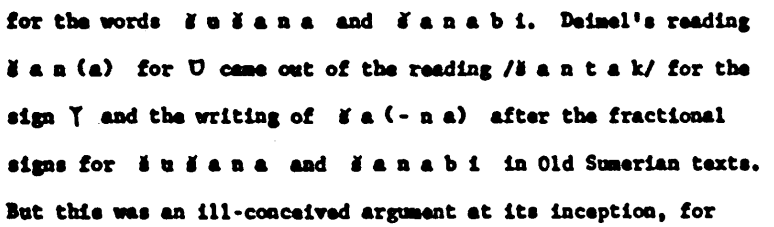
\includegraphics[width=0.75\textwidth]{powell-107.png}
  \caption{Discussion of the readings of proposed {\oneDišC}
  and already-encoded {\xsuxfont 𒁹} in \cite[107]{Powell1971}.\label{powell107}}
  \end{center}
\end{figure}
\begin{figure}[H]
  \begin{center}
  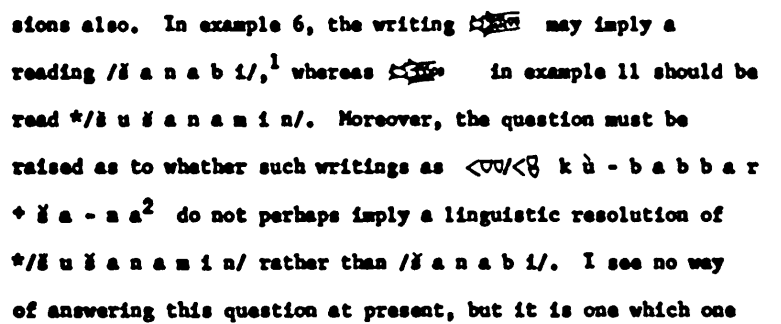
\includegraphics[width=0.75\textwidth]{powell-138.png}
  \caption{Discussion of the readings of proposed {\oneThirdCV} and {\twoThirdsCV} as well as
  already-encoded {\xsuxfont 𒑝} and {\xsuxfont 𒑞} in \cite[138]{Powell1971}.}
  \end{center}
\end{figure}
\begin{figure}[H]
  \begin{center}
  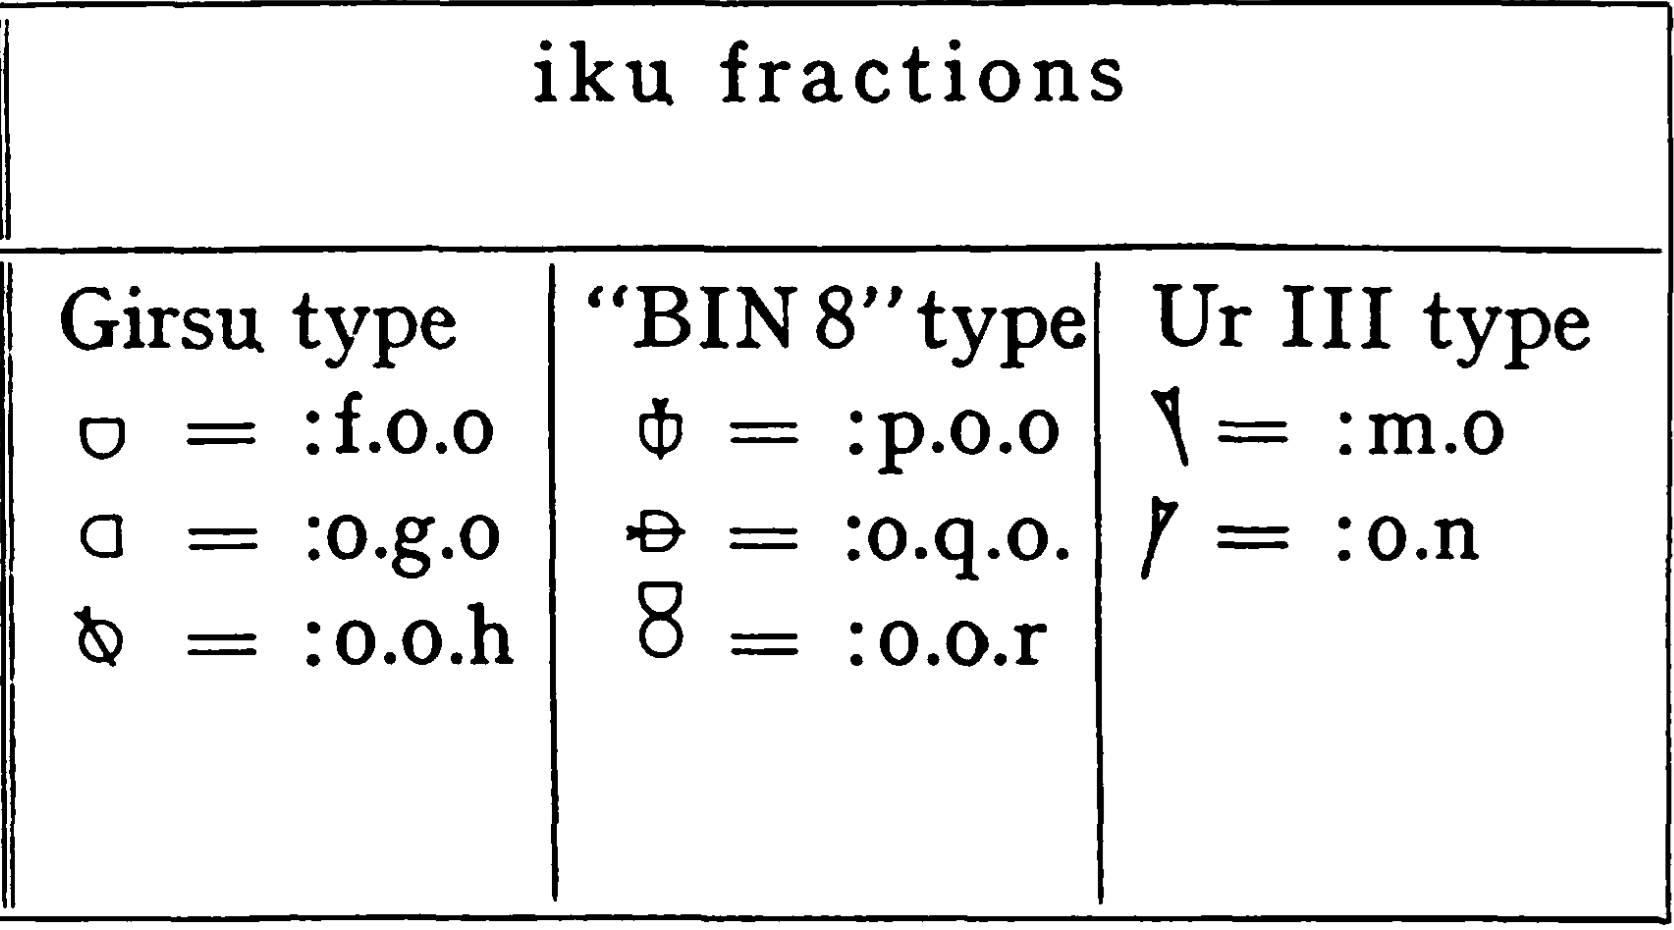
\includegraphics[width=0.75\textwidth]{powell-216.png}
  \caption{A transliteration system for the fractions of the iku in \cite[216]{Powell1972}.}
  \end{center}
\end{figure}
\begin{figure}[H]
  \begin{center}
  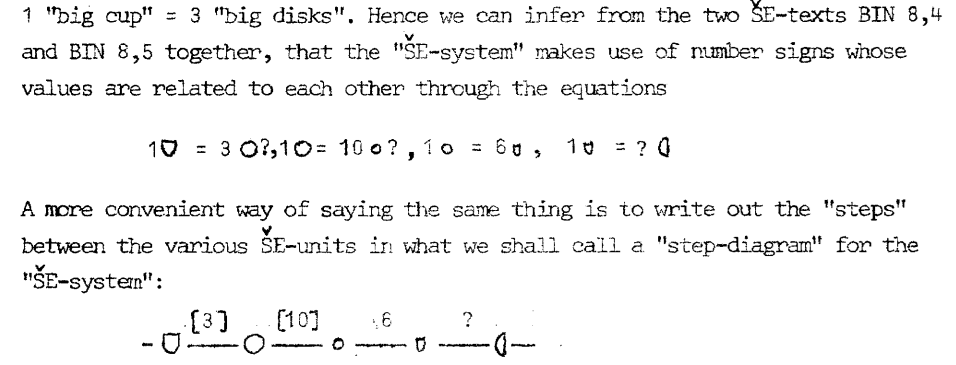
\includegraphics[width=0.75\textwidth]{friberg-10.png}
  \caption[]{The first factor diagram, in \cite[10]{Friberg1978}.\label{firstStepDiagram}}
  \end{center}
\end{figure}
\begin{figure}[H]
  \begin{center}
  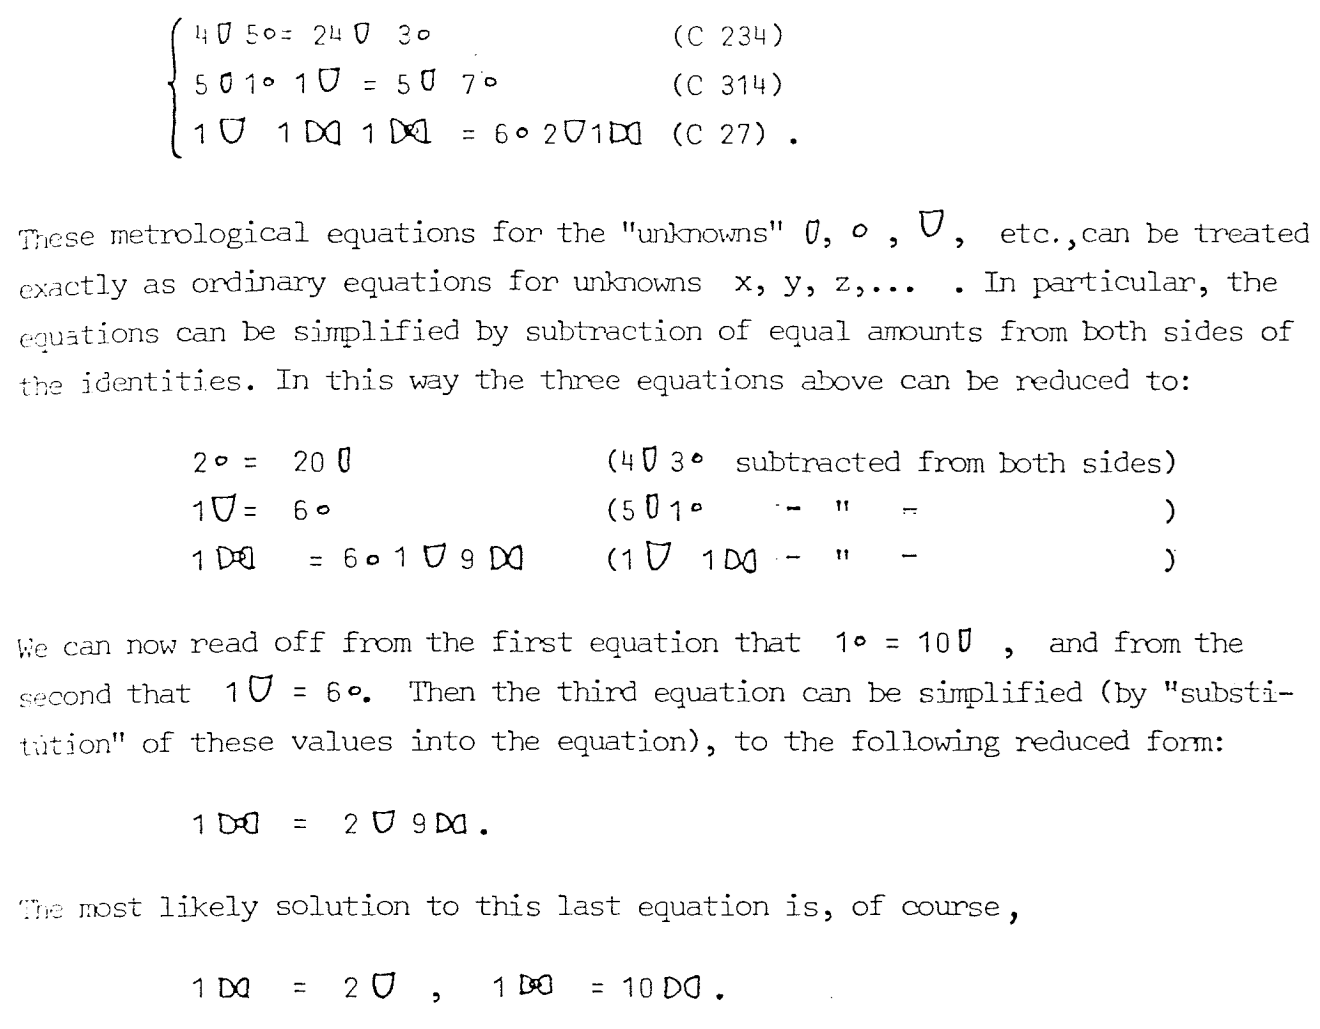
\includegraphics[width=0.75\textwidth]{friberg-15.png}
  \caption[]{The derivation of the factors of the bisexagesimal system in \cite[15]{Friberg1978}\label{FribergEquations}\footnotemark.}
  \end{center}
\end{figure}
\footnotetext{
  The bisexagesimal system is used alike in proto-Elamite and proto-cuneiform texts, see \cite[38]{Friberg1978};
  the derivation in \cite[15]{Friberg1978} is based on proto-Elamite artefacts.
  There is a typo in the equation for C~27:
  the right-hand side should have $10\text{\rotatebox[origin=c]{270}{\oneNFiftyOneC}}$
  rather than $1\text{\rotatebox[origin=c]{270}{\oneNFiftyOneC}}$,
  otherwise nothing could be deduced about \rotatebox[origin=c]{270}{\oneNFiftyOneC}.
  Note that in Friberg’s early works \cites{Friberg1978}{Friberg1979}{Friberg1986}{Friberg1987},
  copies of fourth millennium and sometimes third millennium tablets are shown as vertical text
  (which they were for the scribes),
  and their numerals are written within horizontal text in the same orientation
  that they have if the tablet is taken as vertical text; in \cite{UAX50} parlance, as
  if they had Vertical\_Orientation=Upright. In addition, they are listed in these equations in the horizontal order
  in which they appear as vertical text (thus the rightmost numeral is the most significant, read first).
  Cuneiform is correctly Vertical\_Orientation=Rotated,
  consistently both with modern practice and with the rotation between earlier vertical and later horizontal monumental inscriptions.
  Friberg’s early conventions are not followed in later scholarship,
  and are abandoned in his own more recent works, such as \cite{Friberg2007}; a more typical way to express the first equations might be
  \begin{align}
    5\text{\oneUC}+4\text{\oneAšC}&=3\text{\oneUC}+24\text{\oneAšC}
    \tag{\text{C 234}}\\
    1\text{\oneŊešTwoC}+1\text{\oneUC}+5\text{\oneAšC}&=7\text{\oneUC}+5\text{\oneAšC}
    \tag{\text{C 314}}\\
    1\text{\oneNFiftyFourC}+1\text{\oneNFiftyOneC}+1\text{\oneŊešTwoC}&=10\text{\oneNFiftyOneC}+2\text{\oneŊešTwoC}+6\text{\oneUC}\text.
    \tag{\text{C 27}}
  \end{align}
  A diplomatic edition of \cite{Friberg1978} could rotate the numerals using a higher-level protocol:\usetagform{fribergFullStopTwentySeven}
  \begin{empheq}[left=\empheqlbrace]{align}
    % derived from the above as print('\\\\\n'.join('='.join('~'.join(reversed([term.replace('}','}}').replace(r'\text{',r'\text{\rotatebox[origin=c]{270}{') for term in side.split('+')])) for side in line.strip().split('&=')) for line in s.split(r'\\')))
    &4\text{\rotatebox[origin=c]{270}{\oneAšC}}~5\text{\rotatebox[origin=c]{270}{\oneUC}}=24\text{\rotatebox[origin=c]{270}{\oneAšC}}~3\text{\rotatebox[origin=c]{270}{\oneUC}}
    \tag{\text{C 234}}\\
    &5\text{\rotatebox[origin=c]{270}{\oneAšC}}~1\text{\rotatebox[origin=c]{270}{\oneUC}}~1\text{\rotatebox[origin=c]{270}{\oneŊešTwoC}}=5\text{\rotatebox[origin=c]{270}{\oneAšC}}~7\text{\rotatebox[origin=c]{270}{\oneUC}}
    \tag{\text{C 314}}\\
    &1\text{\rotatebox[origin=c]{270}{\oneŊešTwoC}}~1\text{\rotatebox[origin=c]{270}{\oneNFiftyOneC}}~1\text{\rotatebox[origin=c]{270}{\oneNFiftyFourC}}=6\text{\rotatebox[origin=c]{270}{\oneUC}}~2\text{\rotatebox[origin=c]{270}{\oneŊešTwoC}}~1\text{\rotatebox[origin=c]{270}{\oneNFiftyOneC}}
    \tag{\text{C 27}}
  \end{empheq}}
\begin{figure}[H]
  \begin{center}
  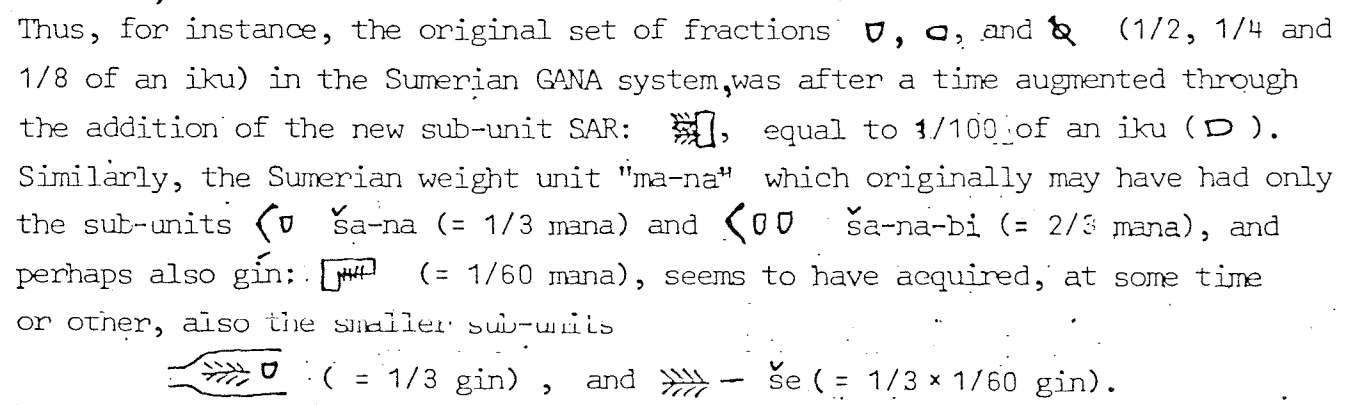
\includegraphics[width=0.75\textwidth]{friberg-49.png}
  \caption{Discussion of proposed fractions
  \oneDišC, \oneQuarterIkuC, \oneEighthIkuC, and \oneThirdCV,
  as well as already-encoded {\xsuxfont 𒑝} and {\xsuxfont 𒑞} in
  \cite[49]{Friberg1978}\label{FribergFractions}.}
  \end{center}
\end{figure}
\begin{figure}[H]
  \begin{center}
  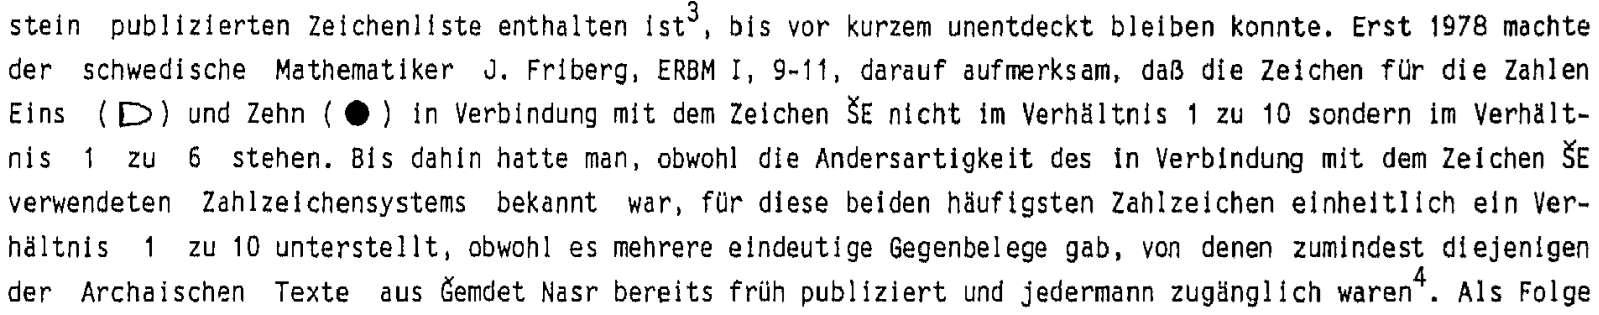
\includegraphics[width=0.75\textwidth]{damerow-englund-117.png}
  \caption{Discussion in \cite[\pno~117]{DamerowEnglund1987} of the discovery in
  \cite[9--11]{Friberg1978} (see Figure~\ref{firstStepDiagram})
  of the different relations between \oneAšC{} and \oneUC{} in systems
  \ref{systemG} and \ref{systemŠ}.}
  \end{center}
\end{figure}
\begin{figure}[H]
  \begin{center}
  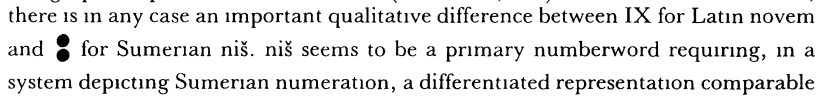
\includegraphics[width=0.75\textwidth]{englund-132.png}
  \caption{The sign \twoUC{} used in a parallel with IX in \cite[\ppno~131--133 \withnote~9]{Englund1988},
  discussing an argument from \cite[172]{Powell1972} on the question
  of the language of the Uruk III texts.\label{EnglundTwoUC}}
  \end{center}
\end{figure}
\begin{figure}[H]
  \begin{center}
  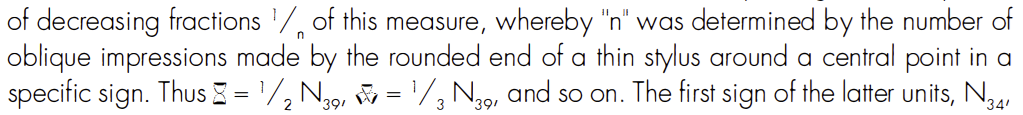
\includegraphics[width=0.75\textwidth]{englund-113.png}
  \caption[]{Description of the fractions \oneNTwentyFour{} and \oneNTwentySix{} in \cite[113]{Englund1998}\footnotemark.\label{englund113}}
  \end{center}
\end{figure}
\footnotetext{The text erroneously has $N_{34}$ instead of $N_{24}$.}
\begin{figure}[H]
  \begin{center}
  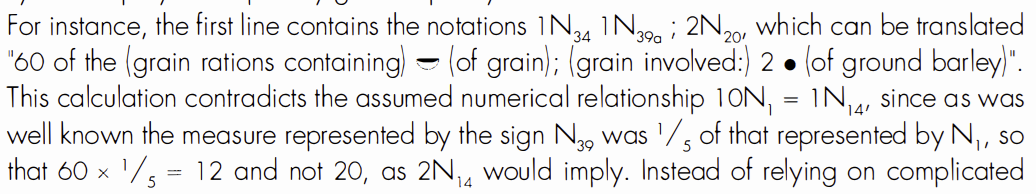
\includegraphics[width=0.75\textwidth]{englund-116.png}
  \caption{The sign \oneNThirtyNineA{} used as a capacity
           measure within otherwise translated text in \cite[116]{Englund1998}.\label{englund116}}
  \end{center}
\end{figure}
\begin{figure}[H]
  \begin{center}
  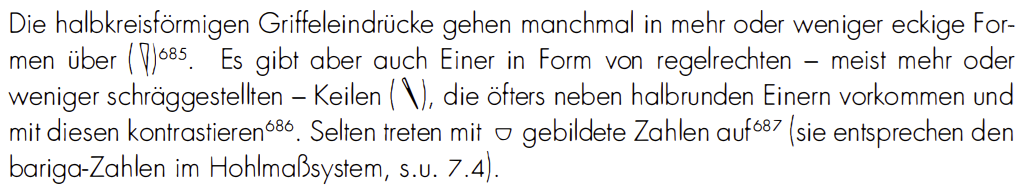
\includegraphics[width=0.75\textwidth]{krebernik-303.png}
  \caption{Discussion of co-occurrences and contrasts between
  {\xsuxfont 𒁹}, {\xsuxfont 𒀹}, and \oneDišC{} in \cite[303]{Krebernik1998}.\label{krebernik303}}
  \end{center}
\end{figure}
\begin{figure}[H]
  \begin{center}
  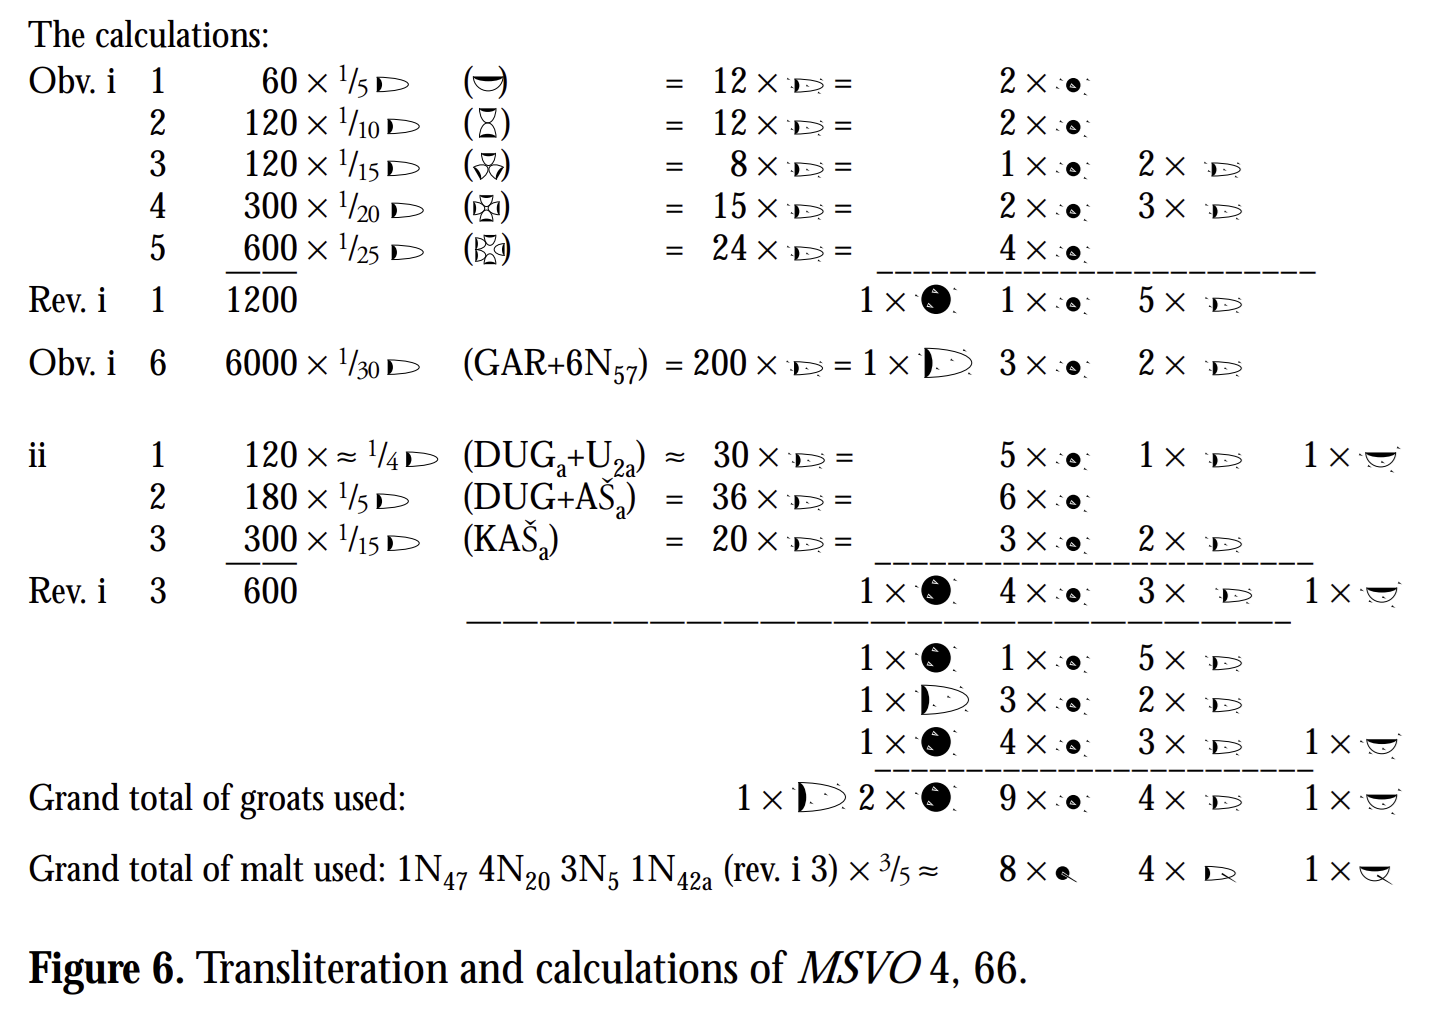
\includegraphics[width=0.75\textwidth]{englund-15.png}
  \caption{Calculations from \cite{P005468} transcribed in \cite[132]{Englund2001} using modern mathematical
  notation combined with some of the proposed characters.\label{englund15}}
  \end{center}
\end{figure}
\begin{figure}[H]
  \begin{center}
  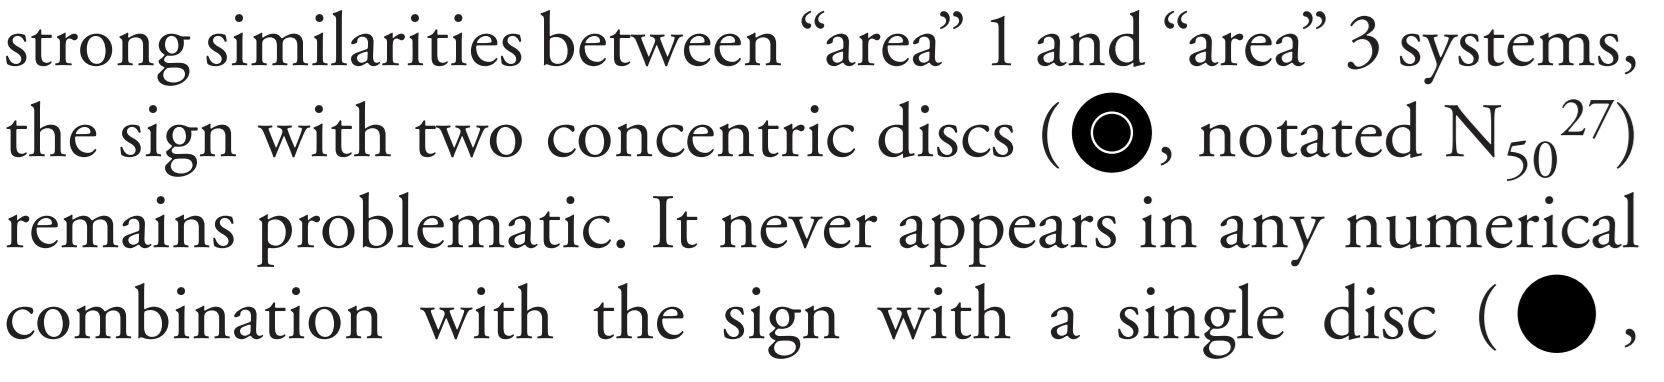
\includegraphics[width=0.75\textwidth]{chambon-6.png}
  \caption[]{Discussion of \oneŠarʾuC{} and \oneŠarTwoC{}\footnotemark{} in \cite[6]{Chambon2003}.\label{chambon6}}
  \end{center}
\end{figure}
\footnotetext{The statement that these do not co-occur refers to the texts from ED I--II Ur;
these signs co-occur both earlier and later in areas,
with different relations as previously discussed.}
\begin{figure}[H]
  \begin{center}
  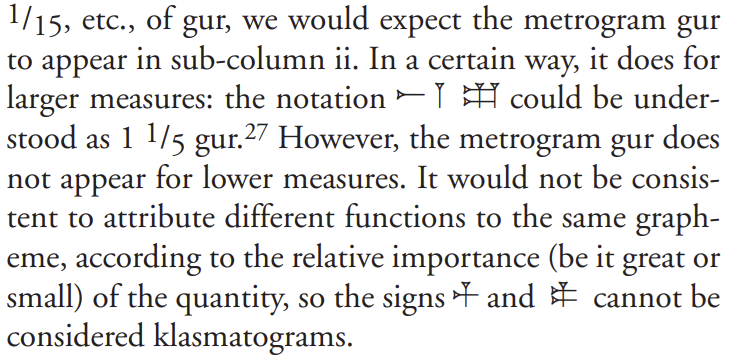
\includegraphics[width=0.375\textwidth]{proust-9a.png}
  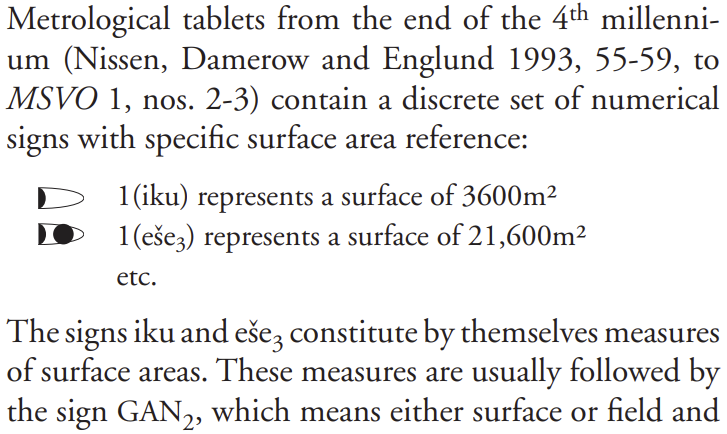
\includegraphics[width=0.375\textwidth]{proust-9.png}
  \caption[]{Discussion of Old Babylonian\footnotemark{} capacity and fourth millennium area measures in \cite[9]{Proust2009}.\label{proust9}}
  \end{center}
\end{figure}
\footnotetext{The cuneiform text is Unicode-encoded.}
\begin{figure}[H]
  \begin{center}
  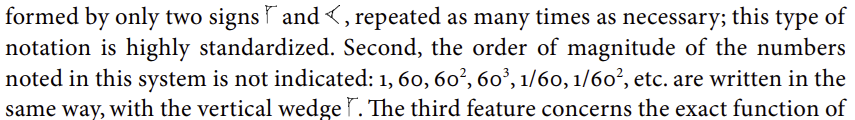
\includegraphics[width=0.75\textwidth]{chambon-58.png}
  \caption{
    Description of the SPVS in \cite[58]{Chambon2012},
    using the already-encoded signs {\xsuxfont 𒁹} and {\xsuxfont 𒌋}.\label{chambon58}}
  \end{center}
\end{figure}
\begin{figure}[H]
  \begin{center}
  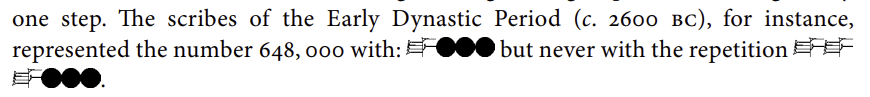
\includegraphics[width=0.75\textwidth]{chambon-59.png}
  \caption[]{Discussion of large numbers illustrated by {\xsuxfont 𒃲\threeŠarTwoC}\footnotemark{} in
                \cite[59]{Chambon2012}\label{chambon59}}
  \end{center}
\end{figure}
\footnotetext{Compare {\xsuxfont 𒊹𒃲} in system~\ref{systemGOB}.
Sign order can be variable in early texts, see \cite[8]{Foxvog2016}. See \cite{P010773}, also discussed in \cite[148]{Friberg2007},
for an example of {\xsuxfont 𒃲\oneŠarTwoC},
and \cites{P274845}{P241764} for examples of {\xsuxfont $n$\oneŠarTwoC 𒃲}.}
\begin{figure}[H]
  \begin{center}
  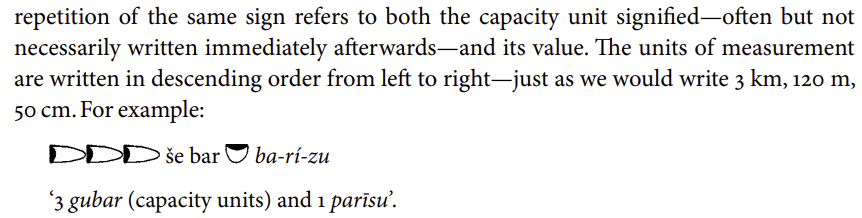
\includegraphics[width=0.75\textwidth]{chambon-61.png}
  \caption{Partial transliteration of \cite[\href{http://ebda.cnr.it/tablet/view/1322\#57724}{\recto~5~3}]{P240597}
  {\xsuxfont\threeAšC{} 𒊺 𒁇 \oneDišC{} 𒁀𒌷𒍪} in \cite[61]{Chambon2012}\label{chambon61}.}
  \end{center}
\end{figure}
\begin{figure}[H]
  \begin{center}
  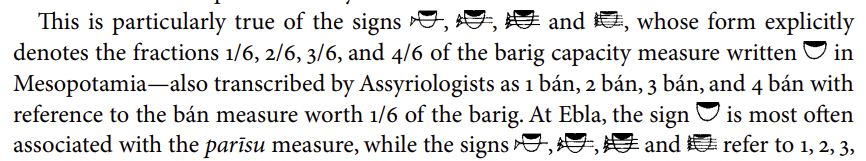
\includegraphics[width=0.75\textwidth]{chambon-63.png}
  \caption{Discussion in \cite[64]{Chambon2012} of the relation between \oneBanTwoC--\fourBanTwoC{} and \oneDišC{} in Mesopotamia and in Ebla.\label{chambon64}}
  \end{center}
\end{figure}

\begin{figure}[H]
  \begin{center}
  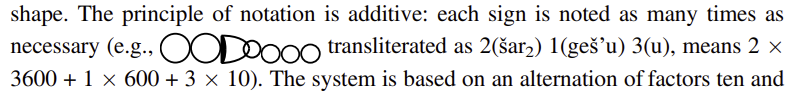
\includegraphics[width=0.75\textwidth]{proust-350.png}
  \caption{Explanation of the structure of the number {\twoŠarTwoC\oneŊešʾuC\threeUC} in \cite[350]{Proust2020}.\label{proust350}}
  \end{center}
\end{figure}

\begin{figure}[H]
  \begin{center}
  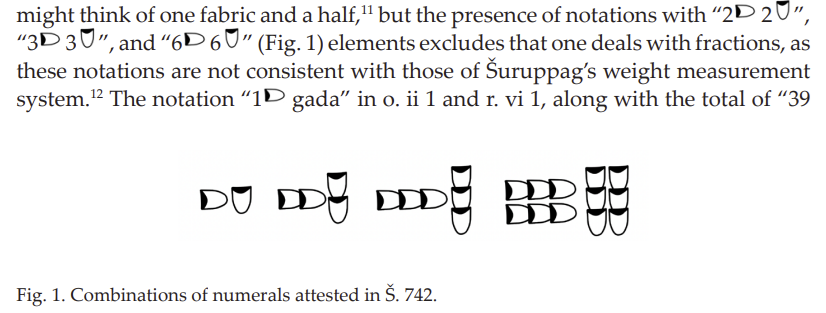
\includegraphics[width=0.75\textwidth]{gori-162.png}
  \caption{Discussion of the contrast between {\oneAšC} and {\oneDišC} numerals in \cite[162]{Gori2023}.\label{gori162}}
  \end{center}
\end{figure}

\begin{figure}[H]
  \begin{center}
  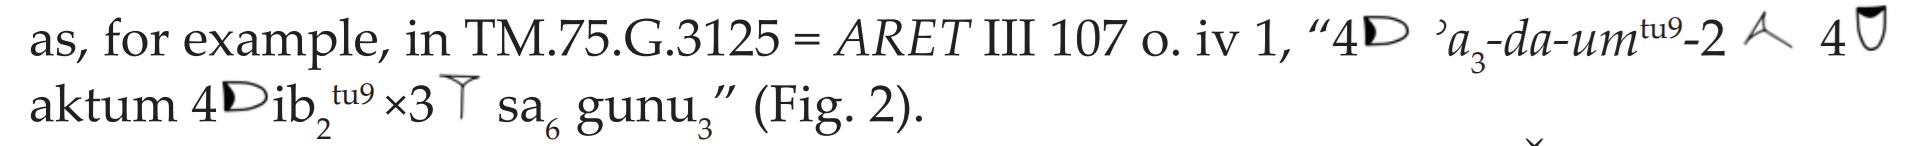
\includegraphics[width=0.75\textwidth]{gori-163.png}
  \caption{Transliteration in \cite[163]{Gori2023} of \cite[\href{http://ebda.cnr.it/tablet/view/217\#13705}{\recto~4~1}]{P242293} incorporating untransliterated numerals.\label{GoriTransliteration}}
  \end{center}
\end{figure}

\subsection{Non-numeric usage}\label{non-numeric}
\epigraph{
{\nafont 𒊕 𒉆𒁾𒊬 𒁹 𒀸𒁉 \hfill 𒅗𒁉 𒐋𒀀𒀭\\
    \hspace*{2em} 𒐕𒀀𒀭 𒁀𒁺 \hfill 𒅗 𒌤𒁉 𒄿𒍪𒌋}\\
{\nafont 𒊑𒌍 𒁾𒊬𒊒𒋾 𒊓𒀭𒋳𒆪 𒅖𒋼 \hfill 𒋗𒌋 \\
    \hspace*{2em} 𒊑𒁶𒋗 𒋀𒅆𒋗 \hfill 𒁹 𒋗𒅆 𒄿𒆲 \\
    \hspace*{2em} 𒉌𒂍𒋢 \hfill 𒋾𒁲𒂊}\\
{The beginning of the scribal art is a single wedge.
That one has six pronunciations;
it also stands for `sixty'\footnotemark. Do you know its reading\footnotemark?}}{Examenstext A}
\addtocounter{footnote}{-1}
\footnotetext{The reader
will recall that ŋeš₂ is written {\xsuxfont 𒐕}, with a larger wedge than {\xsuxfont 𒁹};
however, these signs have merged by the time Examenstext A is composed.}
\stepcounter{footnote}
\footnotetext{
Besides ŋeš₂, a look at \cite{OSL} shows that the values
diš, ge₃, makkaš, saŋtak₄, and tal₄ are attested both in
\cite{ePSD2} and in lexical lists.
The sign is also used for the Akkadian word \emph{ana} in the Neo-Assyrian period.}

Many of the cuneiform numerals are used with a logographic or phonetic value.
For example, the sign {\xsuxfont 𒀸} has, \emph{inter alia}, the values aš, rum, and dili.
While the horizontal numerals are most frequently
written {\oneAšC} in the Early Dynastic period\footnote{A
\cite{CDLI} search for \texttt{"(asz@c)"} finds 3296 ED texts,
while a search for \texttt{"(asz)"} finds 81 ED texts,
of which 46 also contain \texttt{"(asz@c)"}.},
such non-numeric usage is almost\footnote{Exceptions are discussed in §\ref{šar₂}.} always written
{\xsuxfont 𒀸}, for instance:
\begin{itemize}[nosep]
  \item in personal names in administrative texts,
  such as the following, which all contain {\oneAšC} numerals:\begin{itemize}[nosep]
  \item {\xsuxfont 𒀸𒊕} in
  \cites[\reverse~1~5]{P010424}[\obverse~1~5]{P010458}[\obverse~2~5′]{P010459}
  from ED IIIa \smash{\textarabic{أبو صلابيخ}},
  \item {\xsuxfont 𒀸𒉌} in \cite[\obverse~2~5]{P010960} from ED IIIa Šuruppag,
  % \item {\xsuxfont 𒀸𒁯𒌦𒄷} in \cite[\obverse~7~18]{P010964} from ED IIIa Šuruppag, % FIXCDLI Nope, 𒀾
  \item {\xsuxfont 𒆷𒈠𒀸𒁯} in \cite[\obverse~4~3]{P251641} from ED IIIb Adab,
  \item {\xsuxfont 𒅤𒊭𒀸𒁯𒈨} in \cite[\reverse~2~3]{P252866} from ED IIIb Adab,
  \item {\xsuxfont 𒈗𒋗𒀸𒉌} in \cite[\reverse~2~4]{P298637} from ED IIIb Umma;
  \end{itemize}
  \item in the Sumerian word {\xsuxfont 𒌑𒀸} u₂-rum, ``property'' in ED IIIb Ŋirsu administrative texts which contain
    {\oneAšC} numerals, such as
    \cites[\obverse~2~3]{P020006}[\reverse~1~2]{P020008}[\reverse~1~2]{P020018}[\obverse~1~4]{P020024}[\obverse~3~1]{P020030};
  \item in lexical texts:
  \begin{itemize}[nosep]
    \item in the divine name {\xsuxfont 𒀭𒎏𒉾𒀸𒁇} in the lexical texts \cites[\reverse~2~4]{P010570}[\obverse~3~6]{P010572},
      where the entries are prefixed with {\oneAšC}.
    \item in the word {\xsuxfont 𒀸} dili, ``small fish'' in
    \cite[\obverse~2~5]{P010578}, witness to Early Dynastic Fish,
    \item in the same word with a determinative, {\xsuxfont 𒀸𒄩} dili\textsuperscript*{ku₆},
    in \cite[\obverse~4~4; 6]{P010586},
    witness to Early Dynastic Food, which starts with {\oneAšC} numerals.
  \end{itemize}
\end{itemize}

This is a clear contrast between {\xsuxfont 𒀸} and {\oneAšC} in this period,
and genuine ambiguity can arise if it is lost; for instance, the personal name
{\xsuxfont 𒀸𒊕} occurs on its own line in the aforementioned administrative texts;
a line {\oneAšC\xsuxfont 𒊕} would instead be read as ``one slave''.

\subsection{The limited benefits of diachronic encoding for numerals}
\label{limitedBenefitsOfDiachrony}
The argument in favour of diachronic encoding is that it facilitates
interoperability in a variety of use cases,
as we have outlined in §\ref{xsuxModel}.
While these benefits are real and now visible for cuneiform signs,
similar considerations are not generally applicable to curviform numerals.

Diachronic reference works such as sign lists and dictionaries tend to not include numbers,
or when they do, they treat them separately, and include signs such as {\xsuxfont 𒀸}
that have both numeric and non-numeric values in both the main list and the section on numbers.
For instance, \cite[123 \psqq]{KWU} lists all of {\xsuxfont 𒀸}--{\xsuxfont 𒐇} together with
{\oneAšC}--{\nineAšC},
while {\xsuxfont 𒀸}, {\xsuxfont 𒐀}, and {\xsuxfont 𒐁}, and only those, appear at the beginning of the sign list,
since they have non-numeric values\footnote{Non-numeric values of {\xsuxfont 𒀸} were discussed in
§\ref{non-numeric};
{\xsuxfont 𒐀} has the values man₃ and min₅, and is used for the word didli, ``several, various'';
{\xsuxfont 𒐁} has the value eš₆.}.
\cite[58]{PTACE} has the numeric signs {\oneAšC}, {\xsuxfont 𒀹}, {\xsuxfont 𒁹},
whereas non-numeric {\xsuxfont 𒀸} is at the beginning of the sign list,
where its values \emph{aš} and \emph{rum} are listed.
For signs with both non-numeric and numeric usage, \cite{LAK} writes \emph{\textgerman{s. die Zahlz.}}
throughout the main list; LAK~1 {\xsuxfont 𒀸} thus reappears at LAK~829 together with
{\oneAšC}, {\xsuxfont 𒀹}, and {\xsuxfont 𒁹}.
One should note \cite{MZL}, which has numbers throughout the sign list;
but that sign list does not show glyphs predating the Old Babylonian period,
nor does it comprehensively cover the numerals used in the Ur III and Old Babylonian
periods, as, for instance, it does not have {\xsuxfont 𒐒}--{\xsuxfont 𒐔} used in
system~\ref{systemGOB}.

Composite texts rarely have witnesses both from the Early Dynastic period
and later; the kinds of texts that do, chiefly lexical and literary texts, do not
contain numbers to the extent that administrative texts do.
Further, there tend to be changes\footnote{Compare,
\exempligratia, in the \emph{Instructions of Šuruppag},
{\xsuxfont 𒋢𒆳𒊒𒆠 𒌫\oneAšC{} 𒌉𒉌𒊏} / {\xsuxfont 𒈾 𒈾𒈬𒊑𒊑} in
the ED IIIa witness \cite[\obverse~2~7]{P222243}, also discussed
in §\ref{šar₂}, and
{\xsuxfont 𒋢𒆳𒊒𒆠𒂊 𒌉𒉌𒊏 𒈾 𒈾𒈬𒌦𒊑𒊑}
in the OB composite \cite[\nopp6]{Q000782} (translated ``Šuruppag gave instructions to his son''
in \cite[\href{https://etcsl.orinst.ox.ac.uk/cgi-bin/etcsl.cgi?text=t.5.6.1\&display=Crit\&charenc=gtilde\&lineid=t561.p1\#t561.p1}{t.5.6.1, 1--13}]{ETCSL}).
It does not matter for the construction of a
composite text whether this is encoded
{\xsuxfont 𒌫\oneAšC} or {\xsuxfont 𒌫𒀸},
since that word is absent from other witnesses,
and since the surrounding words differ.}
to the text between Early Dynastic
and later witnesses that prevent a diachronic encoding of such composites.
For numerals, the switch from {\oneAšC} to {\xsuxfont 𒁹} numerals prevents
diachronic encoding even if {\oneAšC} were unified with {\xsuxfont 𒀸}.
For instance, the lexical list Early Dynastic Food, already mentioned in §\ref{non-numeric},
contains some numbers, and has a witness from the Old Akkadian period covering
these numbers: \cite[\href{https://oracc.museum.upenn.edu/dcclt/P215653.3}{a~1′--6′}]{P215653};
however, they are written with {\xsuxfont 𒁹} numerals, whereas they are written with
{\oneAšC} numerals in the Early Dynastic witnesses; since {\xsuxfont 𒁹}
and {\xsuxfont 𒀸} are distinct\footnote{Besides the contrasts in numeric usage
mentioned in §\ref{capacity}, these (already-encoded) characters were clearly
not unifiable because of the many contrasts in non-numeric usage between them;
several values of {\xsuxfont 𒀸} which are not shared with {\xsuxfont 𒁹}
have already been mentioned, but perhaps most striking is the fact that,
in the Neo-Assyrian period, {\xsuxfont 𒀸} is used for the preposition \emph{ina}, ``in'', and
{\xsuxfont 𒁹} for the preposition \emph{ana}, ``to''.}
characters, the {\oneAšC}-{\xsuxfont 𒀸} unification does not help. 

% Maybe cite https://cdli.mpiwg-berlin.mpg.de/artifacts/522091 OB witness to ED Plants?

More generally, since numbers are so deeply tied to metrology, and since
metrological systems change between the Early Dynastic and later
periods\footnote{See, \exempligratia, \cites[493]{Powell1987}[55]{Robson2008} on the unification of
metrologies in the Old Akkadian period, resulting in the systems described in
§\ref{metrology}.}, there is little opportunity
for a diachronic representation of numeric quantities.

In the case of analyses such as
\cite[\emph{sub} ``\href{https://github.com/ARomach/Cuneiform-Stylometry/tree/06278f9f9747a897d00fb0418b6eaa14fa573e83\#adding-corpora}{Adding Corpora}'']{Romach2023},
it is interesting to note that numeric expressions are removed prior
to the conversion of the corpus to Unicode cuneiform for further analysis.

\subsection{Compatibility considerations}
\label{compatibility}
A disunification twenty years after the fact,
affecting all numerals, would ordinarily be a serious
compatibility issue.
Fortunately, with the exception of one character discussed below,
we are not aware of any font using curviform glyphs for the
already-encoded numerals.
In fact we are not aware of any font designed for a style earlier than Old Babylonian,
except for fonts mimicking the representative glyphs from the code charts,
which are primarily Ur III, but sometimes earlier or later,
as described in \cite[\href{https://www.unicode.org/reports/tr56/\#Representative_Glyphs}{§2.4}]{UTR56}.
The lack of dedicated Ur III fonts may be explainable by the chart-like fonts\footnote{Most
prominently Noto Sans Cuneiform, a system font on both Windows—as part of Segoe UI Historic—and macOS.}
being good enough for most purposes;
the lack of Early Dynastic fonts, by the aforementioned issues with numeral unification
making the representation of any text with numerals intractable.

\subsubsection{The case of ŠAR₂}\label{šar₂}
The character U+\textcsc{122B9} {\cuneiformComposite 𒊹} \textsc{cuneiform sign shar2}
has a circular reference glyph.

In most texts from the Early Dynastic IIIb and Old Akkadian period\footnote{For example, in personal names:\begin{itemize}[nosep]
%\item \cite[\reverse~5~3]{P010263}, ED IIIa literary; % NOTE(egg): Lisman reads that ḫe, so let’s not go there.
\item {\xsuxfont 𒂗𒆠𒊹𒊏} in \cite[\reverse~1~2]{P020019} from ED IIIb Ŋirsu;
\item {\xsuxfont 𒂄𒈨𒊹𒊏𒁺} in \cite[\obverse~2~9]{P020182}, also from ED IIIb Ŋirsu; 
\item {\xsuxfont 𒊩𒀭𒊹} in \cite[\obverse~3~3]{P222186} from ED IIIb Umma;
\item {\xsuxfont 𒌨𒀭𒀀𒊹} in \cite[\obverse~16]{P235312} from Old Akkadian Umma.
\end{itemize}},
a contrast between non-numeric šar₂ written {\xsuxfont 𒊹}
and numeric $1$(šar₂ᶜ) written \oneŠarTwoC{} can be observed,
similar to the contrast between {\xsuxfont 𒀸} and {\oneAšC}
previously discussed in §\ref{non-numeric}.
However, in lexical lists from Šuruppag and Ebla\footnote{These are
archaizing in other ways, \exempligratia, they have a
{\xsuxfont 𒉇}--{\xsuxfont 𒌆} (NAM₂--TUG₂) split.},
as well as in the \emph{\textfrench{Stèle des vautours}},
non-numeric šar₂ is curviform:\begin{itemize}[nosep]
  \item {\originalNoto 𒀭𒂗𒆠𒊹} and {\originalNoto 𒀭𒂗𒊹𒉡𒄄} in \cite[\obverse~10~10; 11]{P010566};
  \item {\originalNoto 𒊹𒄈} and {\originalNoto 𒀭𒊹𒄈} in \cite[\reverse~3~16; 17]{P010576};
  \item {\originalNoto 𒊹𒄷} in \cite[\href{https://oracc.museum.upenn.edu/dcclt/P240986.44}{\recto~3~3}]{P240986}\footnote{From copy in \cite[ELLes~397]{ELLes}.};
  \item {\originalNoto 𒊹𒊏𒈾} in \cite[\obverse~17~9; 18 11; 22 12]{P222399}\footnote{Note
  however {\xsuxfont 𒀭𒉌 𒊹𒊏} on \cite[\obverse~6~17]{P222399}, see 
  Figure~\ref{vultureSquare}.
  Curviform non-numeric šar₂ is clearly archaizing in ED IIIb Ŋirsu;
  one might suppose that the scribe slipped into their modern ways here.}.
\end{itemize}
\begin{figure}
  \begin{center}
    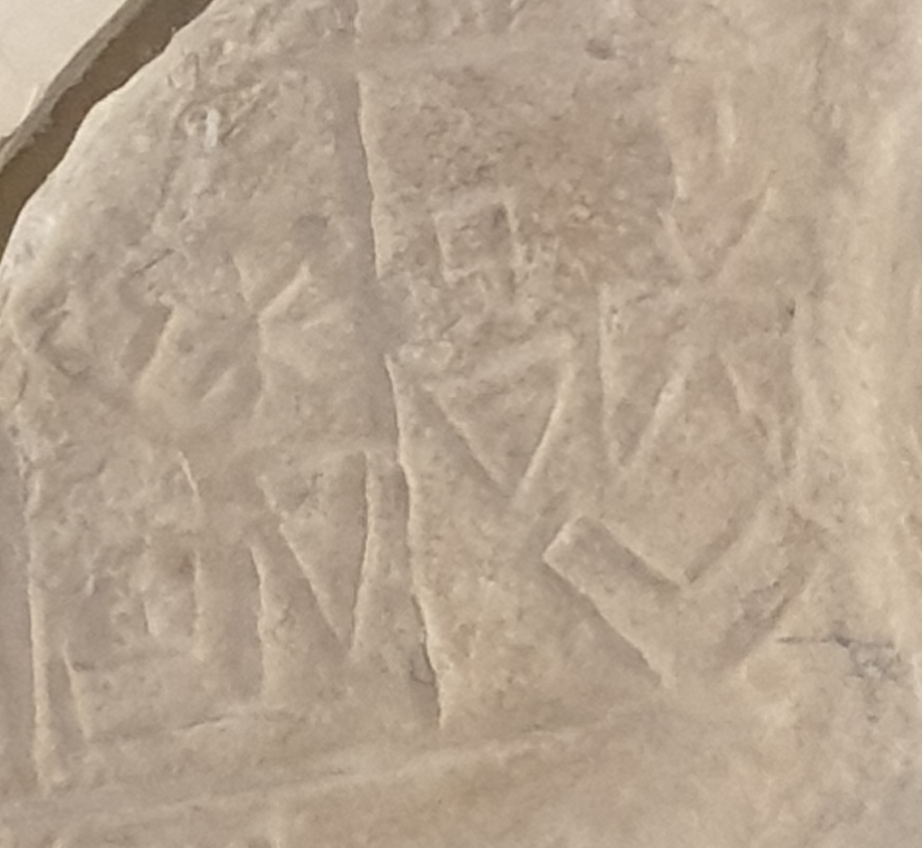
\includegraphics[width=0.5\textwidth]{vautours.png}
    \caption{\cite[\obverse~6~16--17]{P222399} {\xsuxfont 𒃶𒊒𒁉} / {\xsuxfont 𒀭𒉌 𒊹𒊏}.\label{vultureSquare}}      
  \end{center}
\end{figure}

It \emph{would} be disruptive to the diachronic representation of text
if non-numeric šar₂ were to have two different representations.
The character U+\textcsc{122B9} \textsc{cuneiform sign shar2} should therefore be used
in those cases, with its curviform glyph {\xsuxfont 𒊹},
identical to the glyph of the proposed U+\textcsc{12579} \oneŠarTwoC{} \textcsc{CUNEIFORM
NUMERIC SIGN ONE N45}.
Since the archaizing style of texts wherein non-numeric šar₂ is curviform
solidly predates the transition from \oneŠarTwoC{} to {\xsuxfont 𒊹}
in the relevant metrological systems, there is no need to represent
a {\xsuxfont 𒊹}-\oneŠarTwoC{} contrast,
so these characters can have the same glyph in specialist archaizing
Early Dynastic fonts.

Since cuneiform U+\textcsc{122B9} \textsc{cuneiform sign shar2}
effectively merges with U+\textcsc{1212D} {\cuneiformComposite 𒄭} \textsc{cuneiform sign hi},
the reference glyph should remain as it is, \idest, curviform, so that the contrast
between reference glyphs within the Cuneiform block remains clear; see
\cite[\href{https://www.unicode.org/reports/tr56/\#Representative_Glyphs}{§2.4}]{UTR56}.
Since system fonts follow the reference glyphs,
and since extant specialist fonts target styles where U+\textcsc{122B9} is unambiguously cuneiform,
there are no compatibility issues.

Note that in rare cases, such as \cite[\obverse~2~7]{P222243} from ED IIIa Adab,
non-numeric {\xsuxfont 𒀸} (here with the value rum) is written {\oneAšC}.
It is out of scope for this proposal to decide whether
such occurrences should be treated as anomalous spellings, encoded as
U+\textcsc{12550} \oneAšC{} \textcsc{cuneiform numeric sign one N01},
or as stylistic distinctions, encoded as
U+\textcsc{12038} \textsc{cuneiform sign ash} with a curviform glyph.
in practice this would often be determined by the transliteration from which
the cuneiform text is generated; it is noteworthy that as of this writing,
the \cite{CDLI} transliteration (UR2-$1$(aš@c)) and the \cite{ePSD2} one (uru₈\textsuperscript*{rum})
of this word disagree on that aspect.
Since {\xsuxfont 𒀸} has a cuneiform reference glyph,
this does not pose any compatibility concerns.

\subsubsection{Transliteration}
\label{transliteration}
An important feature of the encoding is that, in order to
support input and bulk conversion of transliterated corpora to
Unicode cuneiform, it should not represent distinctions that are finer
than those recorded in typical transliterations; 
thus, while some older forms of BIL₂ can be described as
{\cuneiformComposite 𒉈}×{\cuneiformComposite 𒆜}
NE×KASKAL or {\cuneiformComposite 𒉈}×{\cuneiformComposite 𒉽}
NE×PAP\footnote{As on \cite{P249253}.},
they are typically all transliterated bil₂,
and therefore are all represented by the character U+\textcsc{1224B} {\cuneiformComposite 𒉋}
\textcsc{CUNEIFORM SIGN NE SHESHIG}, its name notwithstanting,
as described in \cite[\href{https://www.unicode.org/reports/tr56/\#Sign_Names}{§2.5}]{UTR56}.

The situation is more complicated for numbers.
Many transliterations do not represent the type of numeral used,
instead interpreting the whole numeric expression and transcribing
it with delimiters or units as needed to disambiguate.
For instance, {\xsuxfont 𒐕𒌍𒐃𒄥} from \cite[\reverse~21]{P305639}
may be transliterated as $95$~gur, as in \volcite{2}[62]{Feuerherm2004}.
The numerals may also be transliterated separately,
but solely by their values in terms of the overt unit,
as in \cite{EbDA} transliterations:
the aforementioned {\twoUC\oneAšC\oneDišC\xsuxfont 𒄘𒁇 𒐌𒃻𒋙𒊕 𒈫𒈦𒀭𒍡𒍝}
from \cite[\href{http://ebda.cnr.it/tablet/view/1379\#61615}{\recto~3~3}]{P240533}
is transliterated ``$20$-$1$-$1/2$~\emph{gu}₂-\emph{bar} $7$~nig₂-sagšu $2$-$1/2$~an-zamₓ\footnote{As
of this writing, \cite{EbDA} actually has an-zamᵪ, with U+\textcsc{1D6A}
\textcsc{GREEK SUBSCRIPT SMALL LETTER CHI}.} \emph{za}'', reading both
\oneDišC{} and {\xsuxfont 𒈦} as $1/2$,
but not distinguishing them.

In particular, these transliterations do not differentiate between
{\xsuxfont 𒀸} and {\xsuxfont 𒁹} numerals, nor between
\oneAšC{} and \oneDišC{} numerals.
For instance, the aforementioned \cite[\href{http://ebda.cnr.it/tablet/view/217\#13705}{\recto~4~1}]{P242293}
{\fourAšC~\xsuxfont 𒂍𒁕𒌝𒌆𒑊 \fourDišC~\xsuxfont 𒀀𒋢 \fourAšC~\xsuxfont 𒔻
𒌆 𒊷𒁯} is transliterated ``$4$~\emph{ʾa}₃-\emph{da}-\emph{um}\textsuperscript*{tug₂}-II $4$~aktum\textsuperscript*{tug₂} $4$~ib₂-III gun₃ sa₆ \textsuperscript*{tug₂}''
in \cite{EbDA}, with no distinction between the \fourAšC{} and \fourDišC.
Since {\xsuxfont 𒀸} and {\xsuxfont 𒁹} numerals are separately encoded,
the numeric expressions in such transliterations cannot be transformed
into Unicode cuneiform without additional context, regardless of
curviform--cuneiform unification.

In metrological systems such as systems~\ref{systemGOB} and~\ref{systemC}
where some units are indicated by the type of numeral
rather than an overt unit sign, it is common practice to add the unit in parentheses
in transliteration; for instance, {\xsuxfont 𒑘𒐃𒀹𒃷𒐌𒊬} from \cite[\obverse~1]{P386847}
is transliterated ``$1$(eše₃) $5\text{½}$~iku\footnote{{\xsuxfont 𒃷} interpreted as a unit, as discussed in §\ref{metrology}.} $7$~sar'' in \volcite{2}[176]{Feuerherm2004},
and {\xsuxfont 𒑗𒑐𒐌𒈦𒋡} from \cite[\obverse~12]{P307255}
is transliterated ``$1$(n\footnote{short for nigida,
an older reading of bariga;
see \cites[376]{Landsberger1950}[181]{Powell1975}[9]{Foxvog2022}.}) $2$(b) $7~\text{½}$~sila₃'' in \volcite{2}[151]{Feuerherm2004}.

This practice has been generalized to systematically indicate numeral shape;
this is in particular the case in \cite{CDLI},
where the transliterations of some the above examples are
``$1$(gesz2) $3$(u) $5$(asz) gur'' for {\xsuxfont 𒐕𒌍𒐃𒄥},
``$1$(esze3) $5$(iku) $1/2$(iku) GAN2 $7$(disz) sar'' for {\xsuxfont 𒑘𒐃𒀹𒃷𒐌𒊬},
and ``$3$(barig) $2$(ban2) $7$(disz) $1/2$(disz) sila3'' for {\xsuxfont 𒑗𒑐𒐌𒈦𒋡}.
\cite{CDLI} and \cite{ePSD2} both distinguish curviform from cuneiform numerals in
transliteration: the length
\vphantom{\scalebox{0.85}{\sixŊešTwoC}}{\smash{\sixŊešTwoC}\threeUC\xsuxfont 𒃻𒁺\oneBanTwoC\xsuxfont 𒑌𒄀}
from \cite[\reverse~2~1]{P020129} is transliterated
``$6$(gesz2@c) $3$(u@c) \{ninda\}nindax(DU) $1/2$(asz@c) $4$(disz@t) gi''
in \cite{CDLI}, and ``$6$(geš₂ᶜ) $3$(uᶜ) \textsuperscript*{ninda}nindaₓ(DU) $1/2$(ašᶜ) $4$(dišᵗ) gi''
in \cite{ePSD2}.
Another example is \cite[39]{Molina2014}, which uses $1a$ for {\xsuxfont 𒀸},
$1d$ for {\xsuxfont 𒁹}, $1ac$ for \oneAšC, $1dc$ or $\text{½}dc$ for \oneDišC{}
depending on reading, etc.
The literature on the Uruk and Early Dynastic I--II periods uses
a different set of transliteration conventions that also
disambiguate numeral shapes,
as will be discussed in §\ref{unificationRationale}.

While there exist transliterations that distinguish {\xsuxfont 𒀸} from {\xsuxfont 𒁹}
but not \fourAšC{} from {\xsuxfont 𒀸}, such as the ones used in \cite{DCCMT},
the trend, especially in more recent works in third millennium studies, seems to be to
represent numeral shape; for example, \cite{Maiocchi2024} gave an example of
the input syntax used by the new ``Urban Economy Begins'' project as
``$10+5\text{c}(\text{GUR})+2(\text{BARIGA})+1(\text{BAN2})$'' for
{\oneUC\fiveAšC\xsuxfont 𒑖𒑏}, with a c
indicating that the GUR numerals are curviform, and the parenthetical
GUR indicating that these are \oneAšC{} rather than \oneDišC{} numerals.
The ``tradition of cavalierly dispensing with numerical notations in notations
of administrative documents'', as \cite[30]{Englund2004} describes it,
seems to be fading.

\subsection{Conclusions}
Co-occurences of curviform and cuneiform numerals are not anecdotal
in the Early Dynastic period, nor are they the result of scribal idosyncrasy.
Instead, they represent systematic contrasts between metrological
systems, between individual units within metrological system, and
between numeric usage and phonetic or logographic usage.
This contrastive usage is reflected in modern publications.
The contrast frequently applies to individual numerals,
rather than to the span of entire numeric expressions.

While it would be technically possible to handle this contrast as
a stylistic distinction, this approach has no real benefit, and
is highly inconvenient, as it would require any treatment of Early
Dynastic administrative texts to use multiple cuneiform fonts, often within
single numeric expressions.
Further, if that contrast is lost in plain-text interchange, the text can
be misinterpreted:
{\xsuxfont 𒌍} is a length of three ropes, but \threeUC{} is an area of three bur₃;
{\oneAšC\xsuxfont 𒁹} could be read as one {\xsuxfont 𒄘𒁇} and one {\xsuxfont 𒃻𒋙𒊕},
where {\oneAšC\oneDišC} would be one and a half {\xsuxfont 𒄘𒁇};
{\xsuxfont 𒀸𒊕} is a personal name, but {\oneAšC\xsuxfont 𒊕} would be ``one slave''.

In addition, there would be a risk of confusion about character identity should
fontmakers attempt to treat the curviform and cuneiform numerals as unified.
A designer concerned about the numeric-syllabic \oneAšC--{\xsuxfont 𒀸} contrast,
and wishing to support diachronic encoding between systems~\ref{systemSOB} and \ref{systemS},
might give the {\xsuxfont 𒁹} numeral series (which is typically only used numerically
in the Early Dynastic period) the glyphs of the \oneAšC{} numeral series,
since the clear {\xsuxfont 𒐕}--\oneŊešTwoC{} identification involves the same rotation;
this would however make it impossible to represent capacity measures that use \oneDišC{}.
Similarly, in an effort to support diachronic encoding for $1/2$(iku),
one might be tempted to give {\xsuxfont 𒀹} the glyph
of \oneDišC{}, thereby rendering the font unusable for quantities measured using
the {\xsuxfont 𒀹} numeral series;
an ED I--II Ur font designer could decide to give {\xsuxfont 𒐴}
the same glyph as {\xsuxfont 𒐬} (that of the proposed \oneŠarʾuC), according to the older area system,
making it impossible to represent the newer system.

At the same time, contrary to most disunifications,
the separate encoding of curviform numerals poses no serious compatibility issues
for existing fonts or encoded corpora,
nor does it, in general,
introduce new issues with transliterated third millennium corpora.
The oddity of {\originalNoto 𒊹} requires some explanation,
but does not pose any architectural issues,
and is not fundamentally different from the other mergers and splits
encountered in the cuneiform script.

\section{Rationale for ED–Uruk numeral unification}
\label{unificationRationale}
A complete rationale for disunification between the non-numeric signs used
in the fourth millennium and the already-encoded cuneiform signs will
be given in the forthcoming proto-cuneiform encoding proposal.
The core issue with extending the cuneiform script further back in time
is that, since 1987, fourth millennium studies have used a different model
of character identity and associated transliteration conventions,
with names being given to structurally different glyphs, and no attempt being made
at assigning phonetic values to them.

This is not a mere classification of glyph variants, as contrastive meanings
of these systematic variants can often be reconstructed,
with, \exempligratia, signs KAŠ\textsubscript*{a}, KAŠ\textsubscript*{b}, and
KAŠ\textsubscript*{c}, depicting filled jars with a spout (a), a handle (c),
or neither (b), being understood as referring to containers of different substances,
see \cite[34\psq]{Englund2001}.
However, not all identified systematic variants are understood, and the general
approach to character identity is closer to that used for undeciphered or
partially deciphered scripts.

As part of the development of these conventions,
a classification of fourth millennium numeric signs was developed; see \cite{DamerowEnglund1987}.
This classification assigns to each unit numerals an identifier formed by the letter $N$ with a numeric subscript
(sometimes with an additional alphabetic subscript):
$N_1$ is \oneAšC, $N_{14}$ is \oneUC, $N_{34}$ is \oneŊešTwoC, etc.
Transliterations of numeric expression then use those to identify the type of number used,
thus $5N_1$ is \fiveAšC, and $5N_{14}$ is \fiveUC.

In contrast with the use of parenthetical unit names,
this approach does not require interpreting the quantity being counted.
This is valuable in contexts where numerals are being used atypically,
as conventional transliterations can otherwise force a dubious interpretation.
For instance, the \cite{CDLI} transliteration of \threeAšC\threeDišC{\xsuxfont 𒌆}  or \sixAšC\sixDišC{} in
\cite[\reverse~1~6;2~2]{P283802} currently uses (barig@c) for the vertical numerals,
since \oneDišC{} numerals are typically capacity measures;
but \cite{Gori2023} interprets these instead as counting linen textiles.
As a result, the fourth millennium conventions for numeral transliteration
are used in Early Dynastic texts, especially those from the ED I--II period,
even though the Sumerian text uses classical assyriological transliteration conventions;
see \cite[\pno~6 \withnote~27]{Chambon2003}.

While the non-numeric signs are treated as undeciphered,
the metrological systems used in the fourth millennium are well understood,
as can be seen in \cite[165]{DamerowEnglund1987}.
As a result, contrary to the non-numeric proto-cuneiform conventions,
these numeric transliteration conventions are compatible with the classical ones described in
§\ref{transliteration}; they are indeed used interchangeably, as in \cite{P011104} % https://oracc.museum.upenn.edu/epsd2/admin/ed12/P011104
which uses the notation u@f in \cite{ePSD2}, but N14@f in \cite{CDLI}.
Indeed, the numerals are used similarly in Early Dynastic metrological systems,
and are visually identical.

A disunification of numerals between the third and fourth millennium would
therefore induce confusion as to which numerals should be used in third millennium
studies, and would needlessly duplicate the encoding of at least seventy characters;
by splitting the attestations, these separate encoding proposals would run into additional
difficulties to supply evidence for encoding.

Note that the structural variants designated by letters in fourth millennium notation have systematically
been encoded, as they have occasionally be found to carry distinct numeric meaning.
For instance, \oneNThirtyC{} $N_{30c}$ is listed as a variant of \oneNThirtyA{} $N_{30a}$ in
\cite[166]{DamerowEnglund1987}, where the numeric value of either in relation to \oneNThirtyNineA{} $N_{39a}$  is still unknown,
but their values are found in \cite[33]{Englund2004} to be $\text{\oneNThirtyC}=\frac{1}{10}\text{\oneNThirtyNineA}$, whereas
$\text{\oneNThirtyA}=\frac{1}{6}\text{\oneNThirtyNineA}$.

\section{Considerations on individual numeral series}\label{extraIdentity}
Usages of the characters U+\textcsc{12550}--U+\textcsc{12597},
under subheadings ``Common Numerals'', ``Numerals used for land areas'',
and ``Early Dynastic capacity measures'', have already been discussed in
§\ref{earlyMetrology}.
The variant forms of fractions of the iku are not unifiable with the ordinary ones:
\oneHalfIkuCV{} is never used as a capacity measure, nor as one half in any other metrological system,
contrary to \oneDišC{}.

The character {\xsuxfont \oneBanTwoC} represents both the usages
\smash{$\frac12$} and $1~\text{ban₂}$, whereas
U+\textcsc{12226} {\cuneiformComposite 𒈦} \textcsc{CUNEIFORM SIGN MASH}
and U+\textcsc{1244F} {\cuneiformComposite 𒑏} \textcsc{CUNEIFORM NUMERIC SIGN ONE BAN2} are disunified.
This disunification is motivated by the unrelated origins of
maš (logographic, meaning ``goat''), always resembling {\xsuxfont 𒈦},
and $1~\text{ban₂}$, descended from {\xsuxfont \oneBanTwoC}.
One could argue that based on their etymologies,
U+\textcsc{1244F} would make more sense
as the sign used for $\frac12$,
but U+\textcsc{12226} is used as the transliteration MAŠ is frequent,
see, \exempligratia, \cite[165]{Huehnergard2011}.

The signs U+12598 \oneThirdCV{} and U+12599 \twoThirdsCV{} are
used in the ED~IIIb Ŋirsu weight system
for fractions {$\frac13$} and {$\frac23$} of a shekel,
with the already-encoded U+\textcsc{1245D} \smash{\cuneiformComposite 𒑝}
and U+\textcsc{1245E} \smash{\cuneiformComposite 𒑞} used for fractions of
a mina, see \cite{Lecompte2016}.
Note that as usual, the description
$\text{\xsuxfont 𒉒}\times(\text{\xsuxfont 𒊺}+n\text{\oneAšC})$
must be understood as allowing for free variation between
{\xsuxfont 𒊺}, {\xsuxfont 𒆜}, and {\xsuxfont 𒉽}, the last one being the description in \cite{Lecompte2016}.
Compare {\xsuxfont 𒉋}
discussed in \cite[\href{https://www.unicode.org/reports/tr56/\#Sign_Names}{§2.5}]{UTR56},
$\text{{\xsuxfont 𒉈} \emph{šeššig}}=\text{\xsuxfont 𒉈}\times{\text{\xsuxfont 𒉽}}
=\text{\xsuxfont 𒉈}\times{\text{\xsuxfont 𒆜}}$ (the last one in,
\exempligratia, Ebla lexical texts).

The characters U+\textcsc{12550}--U+\textcsc{12597} are used in the
bisexagesimal counting system, whose factor diagram is as follows
\cites[15]{Friberg1978}[165]{DamerowEnglund1987}[28]{NissenDamerowEnglund1993},
with \oneAšC{} being the unit:
\begin{equation}
\text{\oneNFiftySixC}
\xleftarrow{6}\text{\oneNFiftyFourC}
\xleftarrow{10}\text{\oneNFiftyOneC}
\xleftarrow{2}\text{\oneŊešTwoC}
\xleftarrow{6}{\text{\oneUC}}
\xleftarrow{10}{\text{\oneAšC}}
\xleftarrow{2}\text{\oneDišC}\text.
\tag{$B$}
\label{systemB}
\end{equation}
It is well attested in the fourth millennium, but
is also attested in Early Dynastic IIIa Šuruppag.
The reference glyph for \oneNFiftySixC{} is based on the design in \cites{DamerowEnglund1987}{NissenDamerowEnglund1993},
rather than the one in \cites{Englund2004}{archsigns}, as the latter requires the use of grey, whereas the earlier one
is black and white.

The characters U+\textcsc{12597}--U+\textcsc{125B0}, U+\textcsc{125B6}--U+\textcsc{125BD} are used in
the grain capacity system \cites[136--139;165]{DamerowEnglund1987}[28]{NissenDamerowEnglund1993}[4]{Englund2001}[33;39]{Englund2004}:
\begin{equation}
\begin{tikzcd}[row sep=small]
  &&\arrow[lddd, "2" above left, start anchor={west}]\text{\oneNTwentyFour}\\
  &&\arrow[ldd, "3", start anchor={west}]\text{\oneNTwentySix}\\
  &&\arrow[ld, "4", start anchor={west}] \text{\oneNTwentyEight}\\
  \text{\oneŊešʾuC}
  \xleftarrow{10}\text{\oneŊešTwoC}
  \xleftarrow{3}\text{\oneŠarTwoC}
  \xleftarrow{10}\text{\oneUC}
  \xleftarrow{6}{\text{\oneAšC}}
  &\arrow[l, "5"] \overunderset{\text{\normalsize\oneNThirtyNineA}}{\text{\normalsize\oneNThirtyNineB}}{\rotatebox[origin=c]{90}{\ =}}
  &\\
  &&\arrow[lu, "5" above right, start anchor={west}]\text{\oneNTwentyNineA}\mathrlap{\questeq\text{\oneNTwentyNineB}}\\
  &&\arrow[luu, "6" above right, start anchor={west}]\text{\oneNThirtyA}\\
  &&\arrow[luuu, "10", start anchor={west}]\text{\oneNThirtyC}\text.
\end{tikzcd}
\tag{\text{\textit{Š}}}
\label{systemŠ}
\end{equation}
The signs U+\textcsc{125B1}--U+\textcsc{125B5} are listed together with them
in \cite[29]{Englund2001} under
``dry cereal products and rations: numerical signs in ideographic use''.

The characters U+\textcsc{125BE}--U+\textcsc{125D0} are used
in a variant of system~\ref{systemS}
used to count dead animals, see
\cites[139]{DamerowEnglund1987}[28]{NissenDamerowEnglund1993}[\pno~40 \withnote~23]{Englund2004}:
\begin{equation}
\text{\oneNThirtyFive}
\xleftarrow{6}{\text{\oneNFifteen}}
\xleftarrow{10}{\text{\oneNTwo}}\text.
\tag{$S'$}
\label{systemSprime}
\end{equation}
The highest attested number in this system is \fiveNThirtyFive\sixNTwo, $306$ dead sheep, in \cite{P006365}.

The characters U+\textcsc{125D1}--U+\textcsc{125E9} are used
in a variant of the bisexagesimal system, see
\cites[165]{DamerowEnglund1987}[28]{NissenDamerowEnglund1993}.

The characters U+\textcsc{125EA}--U+\textcsc{125FC} are used
in a variant of system~\ref{systemŠ} probably used to measure malted barley,
see \cites[139]{DamerowEnglund1987}[29]{NissenDamerowEnglund1993}[\pno~17 \withnote~30]{Englund2001}.
The characters U+\textcsc{125FD}--U+\textcsc{12621} are used
in a variant of system~\ref{systemŠ} probably used to measure emmer,
see \cites[\pno~140; \pno~155 \withnote~67]{DamerowEnglund1987}[29]{NissenDamerowEnglund1993}.
The characters U+\textcsc{12622}--U+\textcsc{12641} are used
in a variant of system~\ref{systemŠ} probably used to measure barley groats,
see \cites[141]{DamerowEnglund1987}[29]{NissenDamerowEnglund1993}[\pno~3 \withnote~7;\pno~17 \withnote~30]{Englund2001}.

The characters U+\textcsc{12642}--U+\textcsc{1264A} are used
in a system whose function is unknown, attested only in the Uruk IV period,
see \cites[143\psq]{DamerowEnglund1987}[27\psq]{NissenDamerowEnglund1993}:
\begin{equation}
\text{\oneUC}
\xleftarrow{10}\text{\oneAšC}
\xleftarrow{2}\text{\oneNTwentyFour}
\xleftarrow{2}\text{\oneDišC}
\xleftarrow{4}{\text{\oneNSevenB}}
\xleftarrow{?}{\text{\oneNNine, \oneNEleven, \oneNTwelve}}\text.
\tag{$E$}
\label{systemE}
\end{equation}

The ``flat'' characters U+\textcsc{1264B}--U+\textcsc{12685}
are used in various metrological systems in ED~I--II Ur,
see the factor diagrams in \cite[4\psq]{Chambon2003}.
\section{Characters not included in this proposal}
\label{notIncluded}
Some numerals previously proposed in \cite{L2/23-190},
as well as some other numerals known to exist in the third millennium,
are not included in this proposal.
Some should be proposed at a later date; others
are likely not encodable.
% FIXCDLI P271238 o ii 6 is 1/3(asz@c), not @v.
\subsection{Fourth millennium numerals}
The following eight numeral series
from \cite[166]{DamerowEnglund1987} are not included;
they are all listed as under \emph{\textgerman{Nichteinordenbare Zahlzeichen}} in \cite[147]{DamerowEnglund1987}.
On these (and two others, possibly $N_{57}$ and $N_{58}$), \cite[27]{NissenDamerowEnglund1993} write
``Ten of the sixty numerical signs contained in the list in figure 27,
moreover, do not belong to any of the identified systems. Three of
them were apparently scribbled by an awkward pupil. As to four
of those remaining, we are not sure whether they constitute
derivations of other, as yet unknown numerical signs or whether
they are in fact numerical signs at all. For at least two of the ten
signs, [$N_{23}$] and [$N_{43}$], we can affirm that each formed part of two
additional systems, about which we know nothing due to the fact
that no informative texts have been unearthed with notations in
these systems.''
\begin{itemize}
  \item $N_{13}$ \rotatebox[origin=c]{90}{\oneNFour}.
  \cite[147]{DamerowEnglund1987} mentions \cite{P002551} as the only attestation.
  \cite{CDLI} now transliterates this \texttt{2(N04)},
  not in \cite{archsigns}. Presumably representable as a rotated \oneNFour, as here.
  \item $N_{16}$ and $N_{17}$.
  Described as ``\emph{\textgerman{vermutlich mit ideographischer Funktion}}'' in \cite[147]{DamerowEnglund1987}.
  $N_{17}$ is only attested in \cite{P000524}, a witness to \cite{Q000028}.
  $N_{16}$ is attested in similar context in the same \cite{P000524},
  but also in other artefacts, including \cite{P283918} and \cite{P283919}
  where notes by Englund in the \cite{CDLI} transliteration suggest it is numeric,
  equal to $\frac{1}{20}\text{\oneNThirtyNineA}$. $N_{16}$ should probably be encoded
  in the Archaic Cuneiform Numerals block.
  \item $N_{23}$. In the current transliterated
  \cite{CDLI} corpus, attested in one Uruk~V artefact,
  and four Uruk~IV artefacts.
  Similar in shape to proto-Elamite $N_{23}$,
  which is well-attested (53~artefacts) and well-understood (part of a decimal system, where it means $100$).
  Best encoded as part of a proto-Elamite proposal,
  where we would clearly have $1$--$9$,
  and given appropriate Script\_Extensions.
  \item $N_{43}$; according to \cite[147]{DamerowEnglund1987},
  probably part of a variant of system~\ref{systemŠ}.
  \item $N_{44}$, $N_{53}$, and $N_{55}$: Only
  attested in \cite{P003855}, which contains no other text.
  Presumably these are the ``awkward pupil'' signs.
\end{itemize}
In addition, the following are not included:
\begin{itemize}
  \item $N_{10}$. Only attested in \cite{P001319} according to
  \cite[143]{DamerowEnglund1987},
  but that text now has $N_{11}$ in its \cite{CDLI} transliteration.
  Not in \cite{archsigns}.
  \item $N_{57}$ and $N_{58}$.
        Dependent on the main proto-cuneiform proposal, whose rationale
        will justify the disunification from {\xsuxfont 𒀸} and {\xsuxfont 𒁹}.
        These should be encoded in a different block to avoid confusion with
        {\xsuxfont 𒀸} and {\xsuxfont 𒁹}, since the Archaic Numerals block
        contains numerals unifiable between Pcun and Xsux.
  \item $N_{59}$. Possibly a variant of \oneNFour{} according to \cite[147]{DamerowEnglund1987}.
  \item $N_{30b}$. Not attested in \cite{CDLI} transliterations, not included in Englund’s more recent works such as \cite[29]{Englund2001}, nor in \cite{archsigns}.
\end{itemize}

The well-understood U₄ numerals, documented in \cite[136\psqq]{Englund1988}
and listed in \cites{archsigns}{L2/23-190},
have not been included as they are likewise dependent on the disunification of proto-cuneiform,
and should be encoded in a different block to avoid confusion with {\xsuxfont 𒌓}.
Some additional numeral series from \cites{archsigns}{L2/23-190} are not included
due to lack of documentation on their usage.
In general, only numerals that are part of a well-understood metrological system have been included.
In particular, numerals such as $12\text{\oneUC}$ (attested in \cite{P200010})
have not been encoded, since the metrological systems involving \oneUC{} numerals
should allow for a numeral beyond
\nineUC{} ($9\text{\oneUC}$).

In addition, numerals that are not attested have not been included, unless
they are part of a series where higher numerals in the metrological system are
attested; thus the unattested \smash{\threeNThirtyFive{}} and \smash{\fourNThirtyFive{}},
which are not in \cite{archsigns}, are included,
because \smash{\fiveNThirtyFive{}} is attested in \cite{P006365},
in a context where it is clearly used as part of system~\ref{systemSprime}.
However, \texttt{1(N30C\textasciitilde{}b)}, which is in \cite{archsigns},
and is the obvious counterpart of \texttt{\oneNThirtyC} in system~\textit{Š}″,
therefore presumably equal to $\frac{1}{10}\text{\oneNFortyOne}$, is not included,
as it is not attested in \cite{CDLI} transliterations at this time.

\subsection{Third millennium numerals}
The metrological systems from Early Dynastic IIIb Ŋirsu discussed in §\ref{earlyMetrology}
require the numerals $7\text{\xsuxfont 𒀹}$, $8\text{\xsuxfont 𒀹}$, and $9\text{\xsuxfont 𒀹}$,
whereas only {\xsuxfont 𒀹}--{\xsuxfont 𒑎} are encoded.
{\xsuxfont 𒀹} numerals are also used in dates.
The higher numerals are less frequent, as subtractive notation 
is often used instead, \exempligratia,
{\xsuxfont 𒌋𒇲𒀹} rather than $9\text{\xsuxfont 𒀹}$,
or {\xsuxfont \oneAšC 𒂠𒇲𒑊𒄀} rather than {\xsuxfont\oneBanTwoC 𒂠$8$𒀹𒄀},
which is presumably why they are not yet encoded.
However, they are clearly attested and understood enough to be encodable.
They should be encoded in the Cuneiform Numbers and Punctuation block.

Early Dynastic IIIb Ŋirsu regnal years use {\xsuxfont 𒀸}×{\xsuxfont 𒀹} numerals ($1$--$9$).
these are extremely well attested: a \cite{CDLI} search for \texttt{"(|ASZxDISZ@t|)"}
finds 1482 artefacts, all ED IIIb, of which 1447 are from Ŋirsu.
These could be encoded in the Cuneiform Numbers and Punctuation block; together with
$7$--$9\text{\xsuxfont 𒀹}$, this would fill the block.
There are three attestations of {\xsuxfont 𒁁}×{\xsuxfont 𒀹} numerals
for regnal years of {\xsuxfont 𒈗𒍠𒄀𒋛}, one of which is damaged,
and none of which have photographs. Absent further evidence,
these seem unifiable with {\xsuxfont 𒀸}×{\xsuxfont 𒀹}.

Some Old Akkadian artefacts have \oneŊešʾuC×{\xsuxfont 𒆜} (LAK~824)
or {\xsuxfont 𒐞}×{\xsuxfont 𒆜}, which has recently been found to
mean $6000$.
The \cite{CDLI} transliterations do not appear to distinguist the curviform and cuneiform
versions of these signs.
These signs appear to be associated with $6$\oneŊešʾuC{} or $6${\xsuxfont 𒐞}.
Further collation\footnote{In the assyriological sense, not the Unicode sense.}
is needed to understand exactly what needs to be encoded.

\cites[5]{Chambon2003}[61]{Chambon2012} mention a sign resembling a mirrored and rotated
\oneBanTwoC, thus \rotatebox[origin=c]{90}{\reflectbox{\oneBanTwoC}}.
It is transliterated $N_{1'}$ in \cite[5]{Chambon2003}, which documents a metrological system that uses it.
However, we have not been able to locate this sign in the ED I--II Ur corpus
nor in the Ebla corpus, as it is unclear how it is transliterated in \cite{CDLI}
or \cite{EbDA}.  Once found, it will likely be proposed for encoding
in the Archaic Cuneiform Numerals block.
\subsection{Stacking patterns}
\label{stackingPatterns}
The already-encoded numerals in the Cuneiform Numbers and Punctuation block
distinguish some \emph{stacking patterns};
for instance $9\text{\xsuxfont 𒁹}$ is encoded both as U+\textcsc{12446} {\xsuxfont 𒑆} and
as U+\textcsc{1240E} {\xsuxfont 𒐎}.
This is in part due to contrastive usage of stacking patterns.
For instance, besides {\xsuxfont 𒑖} and {\xsuxfont 𒑗} which are characteristic of bariga measures,
four bariga is written {\xsuxfont 𒐉} even where $4${\xsuxfont 𒁹} is written {\xsuxfont 𒐼}, as in
\cites[\obverse~2~3;\reverse~1~17]{P255010}[\obverse~4;\reverse~5]{P292843}.
Another contrast is that between the stacking patterns used in scratch calculations in the SPVS,
often {\xsuxfont 𒁹 𒈫 𒐈 𒐼 𒐊 𒐋 𒑂 𒑄 𒑆 𒌋 𒎙 𒌍 𒑩 𒑪}, and results
in metrological systems,
typically {\xsuxfont 𒁹 𒈫 𒐈 𒐉 𒐊 𒐋 𒐌 𒐍 𒐎 𒌋 𒎙 𒌍 𒐏 𒐐},
occasionally co-occurring as in \cites{P142827}{P142357}.
This separate encoding is also for compatibility with distinctions made in
reference works and in some non-numeric transliterations;
for instance, {\xsuxfont 𒐼} is \cite[MZL~860]{MZL} and has the value limmu,
whereas {\xsuxfont 𒐉} is \cite[MZL~852]{MZL} and  has the value limmu₅.
Numeric\footnote{The Sumerian word
limmu means ``four'', so limmu and limmu₅ are still numbers. The distinction here is between
usage in transliterations of phrases such as {\xsuxfont 𒈗 𒀭𒌒𒁕 𒐉𒁀𒆤}
lugal an-ub-da limmu₅-ba-ke₄ (king of the four quarters) or of names,
and of numeric expressions such as {\xsuxfont 𒐉𒋡} $4(\text{diš})$ sila₃.}
transliterations occasionally distinguish the stacking patterns {\xsuxfont 𒐼 𒑂 𒑄 𒑆 𒑩 𒑪},
as in the \cite{CDLI} transliterations of the aforementioned tablets,
although this is rare; often $4(\text{diš})$ is {\xsuxfont 𒐉} in Ur III,
but {\xsuxfont 𒐼} in the Neo-Assyrian period.

However, the stacking patterns from earlier periods
are not separately encoded; for instance,
in ED IIIb Ŋirsu, {\xsuxfont 𒎙} $2$(u) often has one {\xsuxfont 𒌋} atop another.
These older stacking patterns do not appear to be contrastive,
are not marked in transliteration,
and are not listed separately in sign lists
nor assigned any different values.
There is therefore no evidence of a need to encode them;
instead, they should be considered style variants, and an ED IIIb Ŋirsu font should have
an appropriate glyph for U+\textcsc{12399} {\xsuxfont 𒎙} \textcsc{CUNEIFORM SIGN U U}.

Likewise, many stacking patterns are attested for the curviform numerals proposed in this document,
and it is not proposed to separately encode them.
These distinctions would be incompatible with the state of the art in numeric transliterations,
including those by Englund, who insisted on ``a system of transliteration that reflects in a strict fashion
the physical realities of the cuneiform inscriptions'' \cite[30]{Englund2004},
and they are not needed to represent reference works.
Idiosyncratic stacking patterns are in fact particularly common in Early Dynastic and earlier tablets,
as they are structured in rectangular cases rather than lines,
so that numerals may be laid out across the case in whichever way fits the available space;
this is illustrated in Figure~\ref{cheese}.
Note also that the numerals need to be considerably enlarged in order to reproduce the layout of the
tablets, so that \twoUC{} often spans two lines of cuneiform signs, as shown in Figure~\ref{twentyTwoOxen}.
This is impractical when these numerals are set in text that
contrasts them with the larger \oneŊešTwoC{},
and inconsistent with actual practice when
typesetting these numerals, as illustrated in Figure~\ref{EnglundTwoUC}:
reproducing the layout of tablets is not within the scope of plain text.
\begin{figure}
  \newlength{\cheeseWidth}
  \settowidth{\cheeseWidth}{\rotatebox[origin=c]{270}{\LARGE\twoUC}{\LARGE\oneDišC}{\xsuxfont\scriptsize 𒓻}}
\begin{center}
  \parbox{\cheeseWidth}{%
  \linespread{0}\selectfont{}
  \smash{\rotatebox[origin=c]{270}{\LARGE\twoUC}{\LARGE\oneDišC}{\xsuxfont \rlap{\raisebox{-0.2em}{\scriptsize 𒓻}}\raisebox{0.5em}{\hspace*{1pt}\small 𒋗}}}\vphantom{\scalebox{0.6}{\LARGE\twoAšC}}\\
  \vphantom{\scalebox{0.6}{\LARGE\twoAšC}}\hfill \smash{\xsuxfont\scriptsize 𒋳}\\
  \vphantom{\scalebox{0.6}{\LARGE\twoAšC}}\hfill \xsuxfont \smash{\small 𒉌}\nhphantom{{\small 𒉌}𒂵}\smash{\raisebox{0.5em}{𒂵}}\hphantom{{\small 𒉌}\hspace*{1pt}}}
  \caption{The layout of case \cites[\reverse~2~3]{P011099}; the numeral \twoUC{} is rotated to fit the rounded corner of the tablet.}
  \label{cheese}
\end{center}
\end{figure}
\begin{figure}
\newlength{\twentyTwoOxenWidth}
\settowidth{\twentyTwoOxenWidth}{\scalebox{0.5}[1]{\LARGE\twoAšC}{\xsuxfont 𒄞}}
\begin{center}
  {\LARGE\twoUC}\parbox{\twentyTwoOxenWidth}{%
  \linespread{0}\selectfont{}\vphantom{\scalebox{0.6}{\LARGE\twoAšC}}\smash{\scalebox{0.5}[1]{\LARGE\twoAšC}\raisebox{2pt}{\xsuxfont 𒄞}}\\
  \vphantom{\scalebox{0.6}{\LARGE\twoAšC}}{\hfill\smash{\xsuxfont 𒈬}\smash{\xsuxfont 𒀹}}}
  \caption{The layout of case \cites[\obverse~1~1]{P020066}; the numeral \twoUC{} is spread across two lines.
  The text is read in the order {\twoUC\twoAšC\xsuxfont 𒄞 𒈬𒀹}, ``twenty-two oxen, one year old''.}
  \label{twentyTwoOxen}
\end{center}
\end{figure}
\begin{figure}
\begin{center}
\[
  \text{\nineŊešTwoC}=
  \text{\proposalfont\addfontfeature{Alternate=0}\symbol{"12573}}=
  \text{\proposalfont\addfontfeature{Alternate=1}\symbol{"12573}}
\]
  \caption{Three stacking patterns for U+\textcsc{12573} \textcsc{CUNEIFORM NUMERIC SIGN NINE N34}.
  The one on the left is the reference glyph, used in Uruk III
  \cites[\obverse~1~1b]{P003499}[\reverse~1~2]{P004430}, and widely afterwards, \exempligratia,
  ED~IIIa Šuruppag \cite[\obverse~2]{P010678},
  ED~IIIb Ŋirsu \cite[\obverse~1~3]{P020057},
  Old Akkadian Umma \cite[\obverse~11]{P212464}.
  The ones in the middle and right are used in two Uruk IV tablets
  \cites[\reverse]{P001243}[\reverse~2]{P004500}. All three Uruk examples are transliterated
  $9$(N34) in \cite{CDLI}.}
  \label{9N34StackingPatterns}
\end{center}
\end{figure}

The reference glyphs use stacking patterns that are common in the Early Dynastic period,
but that are also attested in the fourth millennium in the Uruk III period;
the fourth millennium, especially the Uruk IV period, also frequently features numerals that use a more vertical layout,
as illustrated in Figure~\ref{9N34StackingPatterns}.
The later, more horizontal styles were chosen for two reasons:
for the numerals used in the third and fourth millennium,
usage in third millennium scholarship will be more frequent;
and the horizontal layout poses fewer layout difficulties when set
in lines of non-cuneiform text, as most modern scholarship is.
Indeed, the absolute size of the indents \oneAšC, \oneŊešTwoC, \oneUC, and \oneŠarTwoC{}
must remain consistent across the numeral series, lest a \oneŊešTwoC{} numeral be confused with
an \oneAšC{} numeral. Since the single indents are frequently used in running text,
as illustrated in §\ref{modernUsage}, they need to be large enough that
the vertical stacking patterns are impractical.

Variant stacking patterns, if needed, may be handled
at a higher level as stylistic distinctions;
Figure~\ref{9N34StackingPatterns} uses OpenType stylistic alternates,
and Figure~\ref{cheese} rotates the character \twoUC{},
in both cases preserving the plain text backing.

% FIXCDLI bad transliteration 4(barig) for 4(ban2) in P286521
%\subsection{Matters for higher-level protocols}
%Rotated bits:
%https://cdli.mpiwg-berlin.mpg.de/artifacts/101087

\subsection{Other glyph variants not reflected in transliteration}
\begin{figure}
  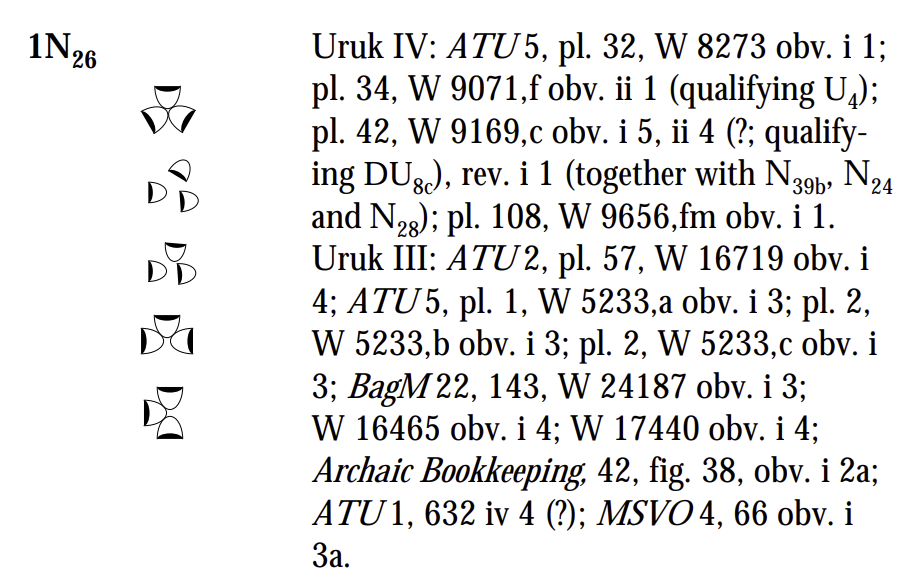
\includegraphics[width=0.375\textwidth]{englund-1(N26).png}
  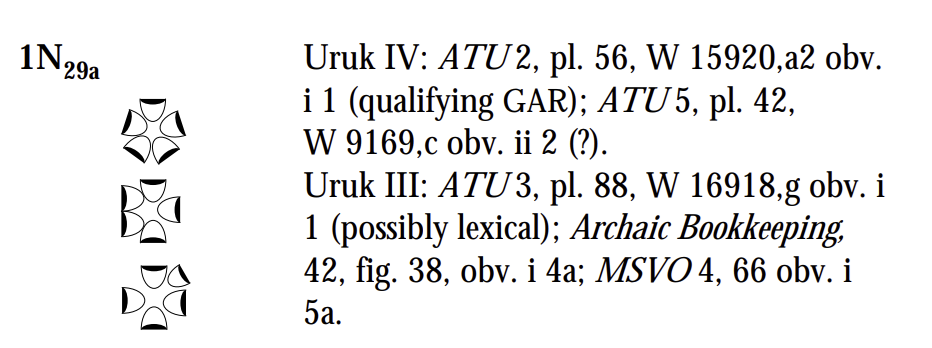
\includegraphics[width=0.375\textwidth]{englund-1(N29a).png}
  \caption{Variants of \oneNTwentySix{} and \oneNTwentyNineA{} from \cite[31]{Englund2001}.}\label{N26-N29a-variants}
\end{figure}
In addition to stacking patterns proper, \cite[128\psq]{L2/23-190} proposes separately
encoding variant glyphs that are not distinguished in transliteration, but listed
but listed together in \cite{archsigns},
thus proposing two characters for \oneNTwentySix{} and two characters for \oneNTwentyNineA{}.
These are merely illustrative of a wide continuum of attested glyphs;
there are additional variants, as shown in Figure~\ref{N26-N29a-variants},
and a cursory search on \cite{CDLI} will find many attestations with further variation in the same vein.
They should not be encoded.
Only the systematic structural variants, which have been distinguished in transliteration
based on a suspicion of distinct semantics, should be encoded.

\section*{Acknowledgements}
\addcontentsline{toc}{section}{Acknowledgements}
TODO(egg): Something about the Vanséveren fonts; acknowledge the reviewers and whoever referred me to relevant literature;
something about the proposal font.
\nocite{DCCLT}
\printbibheading[heading=bibintoc]
\AtNextBibliography{\addfontfeatures{Numbers=Tabular}}
\printbibliography[heading=subbibintoc,title={Artefacts},type=artwork]
%\AtNextBibliography{\addfontfeatures{Numbers=Tabular}}
\printbibliography[heading=subbibintoc,title={ISO and Unicode documents},nottype=artwork,keyword=unicode]
\printbibliography[heading=subbibintoc,title={Online corpora and related projects},nottype=artwork,keyword=reference]
\printbibliography[heading=subbibintoc,title={Other documents},nottype=artwork,notkeyword=unicode,notkeyword=reference]
\end{document}